\chapter{Electron--phonon coupling}\label{chap:6}

The band gap of silicon is \SI{1.17}{eV} at low temperature and \SI{1.12}{eV} at room temperature (\cref{sec:3.3}), and the zero-point motion of the nuclei already lowers it (\cref{sec:6.3}). The static lattice of \cref{chap:3,chap:4} has a gap that changes with neither the temperature nor the nuclear mass, and the harmonic crystal of \cref{chap:5} treats the phonons as a system of their own. The zero-point shift of the gap and the change of the gap with temperature come from the coupling between electrons and nuclei: a displaced nucleus changes the potential the electrons feel, and an electron in turn changes the forces between nuclei. For dark-matter detection this coupling matters well beyond the gap. A phonon can supply the crystal momentum that an electron needs to cross the indirect gap and that a slow incoming particle lacks. The same coupling limits how long an excited carrier keeps its energy before the energy ends up as heat in the lattice. And when a dark-matter particle strikes a nucleus instead of an electron, the coupling decides whether the electrons follow the nucleus or stay behind, excited or ionized; the second outcome is the Migdal effect. All of these effects follow from adding back the couplings that the Born--Oppenheimer approximation of \cref{chap:5} dropped. We will start from those couplings and end, along \cref{fig:6-map}, with the absorption of light, and of dark matter, at the indirect gap of silicon.

\begin{figure}[tbp]
  \centering
  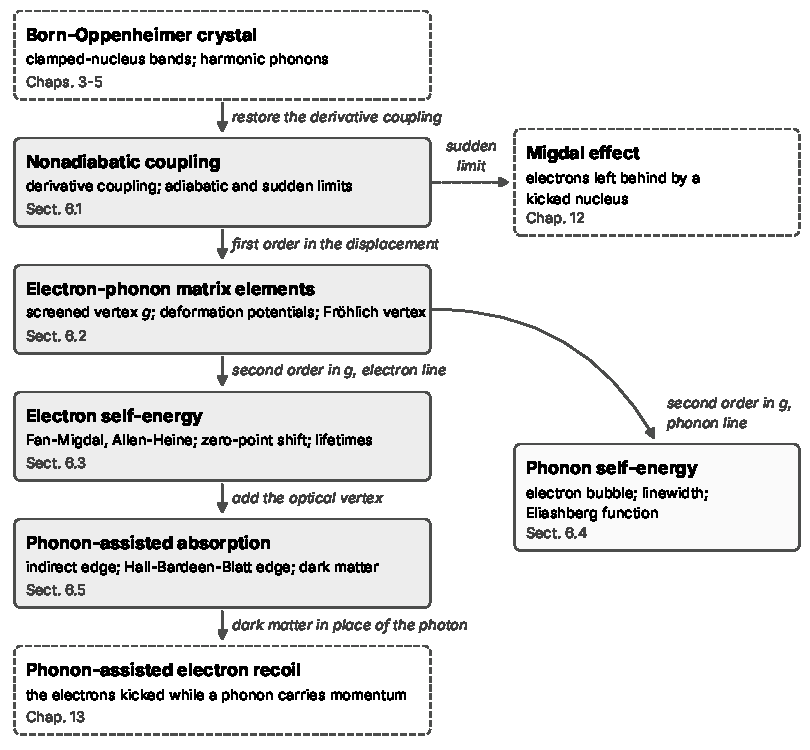
\includegraphics[width=0.85\linewidth]{figures/ch06/map06.pdf}
  \caption{Adding back to the Born--Oppenheimer crystal (\cref{chap:3,chap:5}) what it dropped. The derivative coupling, with its adiabatic and sudden limits (\cref{sec:6.1}), gives at first order in the displacement the electron--phonon vertex $g$ (\cref{sec:6.2}). At second order in $g$ it gives the electron self-energy, with the zero-point shift of the gap and carrier lifetimes (\cref{sec:6.3}), and the phonon self-energy and Eliashberg function (\cref{sec:6.4}). With an optical vertex the derivative coupling gives phonon-assisted absorption at the indirect gap (\cref{sec:6.5}). Dashed boxes: the sudden limit of a kicked nucleus becomes the Migdal effect, and dark matter in place of the photon becomes phonon-assisted electron recoil.}
  \label{fig:6-map}
\end{figure}

\section{Nonadiabatic coupling}\label{sec:6.1}

A dark-matter particle of \SI{1}{GeV} that scatters off a silicon nucleus at the maximum momentum transfer, $q = 2\mu_{\chi N}v_{\mathrm{max}} = \SI{5.10}{MeV}$ (\cref{sec:1.3}), sends the nucleus off at $v_N = q/M = 1.95\times10^{-4}$, or \SI{58}{km.s^{-1}}. The outer electrons of the atom move at typical speeds $\sim\alpha = 7.3\times10^{-3}$, 37 times faster, and the Born--Oppenheimer picture of \cref{sec:5.1} says that they follow the nucleus. They follow it closely but not exactly. Seen from the recoiling nucleus, every electron has suddenly acquired the velocity $-v_N$ and the momentum $m_ev_N = \SI{100}{eV}$, and a cloud bound with momenta $\sim\alpha m_e = \SI{3.7}{keV}$ absorbs that small kick elastically most of the time but not always. For an electron bound as in hydrogen, the probability that it is left excited or ionized is $(v_N/\alpha)^2 = 7\times10^{-4}$. Small as it is, this is the origin of the Migdal effect, which turns a nuclear recoil too small to detect into an electronic signal (\cref{chap:12}). The same couplings, at the slow speeds of thermal and zero-point motion, are what the Born--Oppenheimer approximation drops.

\subsection{Derivative coupling}

The two brackets of \cref{eq:5.1-N} are not independent. Both come from the change of the adiabatic states $\Psi_i(r;u)$ with the displacements. Both can be written through the \emph{derivative-coupling vector}
\begin{equation}
  \vect{d}^{\vect{R}\kappa}_{ji}(u) = \langle\Psi_j|\nabla_{\vect{R}\kappa}\Psi_i\rangle ,
  \qquad \vect{d}^{\vect{R}\kappa}_{ij} = -\vect{d}^{\vect{R}\kappa}_{ji} .
  \label{eq:6.1-d}
\end{equation}
The antisymmetry follows from differentiating the orthonormality $\langle\Psi_j|\Psi_i\rangle = \delta_{ji}$ with respect to a displacement, $\langle\nabla\Psi_j|\Psi_i\rangle + \langle\Psi_j|\nabla\Psi_i\rangle = 0$, together with the reality of the states; in particular $\vect{d}_{ii} = 0$. For the second derivative, we move one gradient to the left. Then we insert the completeness of the adiabatic states at fixed $u$, $\sum_k|\Psi_k\rangle\langle\Psi_k| = 1$:
\begin{equation*}
  \langle\Psi_j|\nabla^2\Psi_i\rangle = \nabla\cdot\langle\Psi_j|\nabla\Psi_i\rangle - \langle\nabla\Psi_j|\nabla\Psi_i\rangle
  = \nabla\cdot\vect{d}_{ji} - \sum_k\vect{d}_{kj}\cdot\vect{d}_{ki}
  = \nabla\cdot\vect{d}_{ji} + \sum_k\vect{d}_{jk}\cdot\vect{d}_{ki} ,
\end{equation*}
where we dropped the label $\vect{R}\kappa$, which every gradient and every $\vect{d}$ carries, and used the antisymmetry in the last step. Inserted in \cref{eq:5.1-N}, the scalar coupling contributes $\nabla\cdot\vect{d}_{ji} + (\vect{d}\cdot\vect{d})_{ji}$, a product of matrices in the state labels, and the derivative coupling $2\vect{d}_{ji}\cdot\nabla$. These are exactly the cross terms of a square. Writing the nuclear wavefunctions $\Psi^{\mathrm{nuc}}_i$ as a column, the nuclear kinetic energy and the couplings of \cref{eq:5.1-coupled} combine into
\begin{equation}
  -\sum_{\vect{R}\kappa}\frac{\nabla_{\vect{R}\kappa}^2}{2M_\kappa}\,\delta_{ji} + \mathcal{N}_{ji}
  = \sum_{\vect{R}\kappa}\frac{1}{2M_\kappa}\Bigl[\bigl(-\ii\nabla_{\vect{R}\kappa} - \ii\vect{d}^{\vect{R}\kappa}\bigr)^2\Bigr]_{ji} ,
  \label{eq:6.1-Pd}
\end{equation}
since $(\nabla + \vect{d})^2 = \nabla^2 + 2\vect{d}\cdot\nabla + (\nabla\cdot\vect{d}) + \vect{d}\cdot\vect{d}$, with $\nabla$ acting on everything to its right. In the adiabatic basis the momentum of a nucleus, $\vect{p}_{\vect{R}\kappa} = -\ii\nabla_{\vect{R}\kappa}$ of \cref{sec:5.3}, becomes the matrix $-\ii(\nabla_{\vect{R}\kappa} + \vect{d}^{\vect{R}\kappa})$. The nucleus carries its electronic state along, and the derivative-coupling vector measures how much of the electronic state changes per unit of displacement, much as a vector potential enters the momentum of a charge. It is a Berry connection, in the space of nuclear displacements instead of crystal momenta. The Born--Oppenheimer approximation keeps only the diagonal part of the matrix, in which $\vect{d}_{00} = 0$ and only the small potential $\mathcal{N}_{00}$ of \cref{app:D.13} survives.

The derivative coupling has a simple reading if we take $\vect{p}/M_\kappa$ to be a velocity, heuristically at first. The off-diagonal, first-order part of \cref{eq:6.1-Pd} is $-(\ii/M_\kappa)\,\vect{d}_{ji}\cdot\vect{p}_{\vect{R}\kappa}$, and on a nuclear wavefunction moving with velocity $\dot{\vect{u}}_{\vect{R}\kappa}$ it acts as $-\ii\,\dot{\vect{u}}_{\vect{R}\kappa}\cdot\vect{d}_{ji}$. The same coupling appears when the nuclei are treated as classical particles that follow a trajectory $u(t)$. The electrons then obey $\ii\partial_t\Psi = H_{\mathrm{el}}(u(t))\Psi$, and we expand $\Psi(t) = \sum_ic_i(t)\,\Psi_i(r;u(t))$ in the adiabatic states at the instantaneous positions. The time derivative falls on the coefficients and, through $u(t)$, on the states, $\partial_t\Psi_i = \sum_{\vect{R}\kappa}\dot{\vect{u}}_{\vect{R}\kappa}\cdot\nabla_{\vect{R}\kappa}\Psi_i$. Projecting on $\Psi_j$,
\begin{equation}
  \ii\dot c_j = E_j(u(t))\,c_j - \ii\sum_i\sum_{\vect{R}\kappa}\dot{\vect{u}}_{\vect{R}\kappa}\cdot\vect{d}^{\vect{R}\kappa}_{ji}\,c_i .
  \label{eq:6.1-tdep}
\end{equation}
The electrons are driven out of their adiabatic state by the velocity of the nuclei times the derivative coupling, and by nothing else. By \cref{eq:5.1-dcoup} the coupling is $\dot{\vect{u}}\cdot\vect{F}_{j i}/(E_i - E_j)$, with $\vect{F}_{ji} = \langle\Psi_j|\nabla_{\vect{R}\kappa}V_{eN}|\Psi_i\rangle$ the matrix element of the force: the power delivered by the nucleus to the transition, divided by the energy the transition costs.

The scalar coupling has no counterpart in \cref{eq:6.1-tdep}. Roughly speaking, it is the quantum correction to a classical trajectory, and compared with the derivative coupling it is suppressed by $|\vect{d}|/(Mv)$, with $|\vect{d}| \sim 1/a_0$ for an electronic state of size $a_0$. A nucleus in its zero-point motion has a momentum $Mv \sim 1/\ell_{\mathrm{zp}}$, and the ratio is $\ell_{\mathrm{zp}}/a_0 \sim \kappa_{\mathrm{BO}}$, which is the extra power of $\kappa_{\mathrm{BO}}$ that separates the scalar from the derivative coupling in \cref{sec:5.1}. A nucleus kicked by dark matter has $Mv_N = q$, and the ratio is $1/(qa_0)$, small for every momentum transfer well above $1/a_0 = \SI{3.7}{keV}$: such a nucleus is a classical projectile as far as its electrons are concerned.

The velocity form also makes the counting of \cref{sec:5.1} transparent. In zero-point motion a nucleus moves at $v \sim \omega_{\mathrm{ph}}\ell_{\mathrm{zp}} \sim (\alpha^2m_e\kappa_{\mathrm{BO}}^2)(\kappa_{\mathrm{BO}}a_0) = \alpha\,\kappa_{\mathrm{BO}}^3$, while the electrons move at $\sim\alpha$. The nuclei are slower than the electrons by $\kappa_{\mathrm{BO}}^3 = (m_e/M)^{3/4}$, which is $2.9\times10^{-4}$ in silicon, and the derivative coupling $v\,|\vect{d}| \sim \alpha^2m_e\,\kappa_{\mathrm{BO}}^3$ is the $\kappa_{\mathrm{BO}}^3$ of the Born--Oppenheimer hierarchy. The kicked nucleus of the opening is 91 times faster than this zero-point estimate, and correspondingly more disruptive.

In a metal the expansion in adiabatic states breaks down at the Fermi surface (\cref{sec:5.1}). What survives is a statement about the electrons that do respond: only those within $\omega_{\mathrm{ph}}$ of the Fermi energy cannot follow the nuclei, a fraction $\omega_{\mathrm{ph}}/E_{\mathrm{F}}$ of the conduction electrons. Since $E_{\mathrm{F}} \sim \alpha^2m_e$ in a typical metal, this fraction is $\sim\kappa_{\mathrm{BO}}^2 = (m_e/M)^{1/2}$, between $10^{-3}$ and $10^{-2}$. The corrections to the electron--phonon interaction that come from these electrons, the vertex corrections, are suppressed by the same ratio. This is Migdal's adiabatic theorem~\cite{migdal1958interaction}; its precise statement with diagrams, and its form for insulators, are given in \cref{sec:6.3}.

\subsection{The electron--phonon Hamiltonian}

The adiabatic basis follows the nuclei and pays with the derivative couplings. The basis of clamped-nuclei states $\Psi_i(r;0)$ does not move, and the coupling sits in the Hamiltonian instead, as the change $V_{eN}(u) - V_{eN}(0)$ of the electron--nucleus potential (\cref{eq:5.1-expand}). This is the form in which the coupling of electrons to phonons is computed and used. Let $v_\kappa(\vect{r})$ be the potential energy of an electron at $\vect{r}$ due to a nucleus of species $\kappa$ at the origin: $-Z_\kappa e^2/(4\pi r)$ for a bare nucleus, or a pseudopotential (\cref{sec:3.5}). With the electron density operator $\op{\nd}_e(\vect{r}) = \sum_e\delta(\vect{r} - \vect{r}_e)$, whose Fourier transform is \cref{eq:2.3-nq},
\begin{equation*}
  V_{eN}(u) = \int\dd^3r\;\op{\nd}_e(\vect{r})\sum_{\vect{R}\kappa}v_\kappa(\vect{r} - \vect{R} - \vect{\tau}_\kappa - \vect{u}_{\vect{R}\kappa}) .
\end{equation*}
To first order in the displacements, $V_{eN}(u) - V_{eN}(0) = \sum_{\vect{R}\kappa}\vect{u}_{\vect{R}\kappa}\cdot\int\dd^3r\,\op{\nd}_e(\vect{r})\,\nabla_{\vect{R}\kappa}V$, with $\nabla_{\vect{R}\kappa}V = -\nabla v_\kappa(\vect{r} - \vect{R} - \vect{\tau}_\kappa)$, the bare force field of one nucleus. We now insert the phonon expansion of the displacement, \cref{eq:5.3-u},
\begin{equation*}
  \vect{u}_{\vect{R}\kappa} = \sum_{\vect{Q}\nu}\frac{\vect{e}_{\kappa\nu}(\vect{Q})\,\ee^{\ii\vect{Q}\cdot\vect{R}}}{\sqrt{2NM_\kappa\omega_{\vect{Q}\nu}}}\,B_{\vect{Q}\nu} .
\end{equation*}
The sum over cells collects the phase factors into a displacement wave of one sublattice,
\begin{equation*}
  \partial_{\kappa,\vect{Q}}V(\vect{r}) = \sum_{\vect{R}}\ee^{\ii\vect{Q}\cdot\vect{R}}\,\nabla_{\vect{R}\kappa}V(\vect{r}) ,
  \qquad \partial_{\kappa,\vect{Q}}V(\vect{r} + \vect{R}') = \ee^{\ii\vect{Q}\cdot\vect{R}'}\,\partial_{\kappa,\vect{Q}}V(\vect{r}) ,
\end{equation*}
where the second relation follows from relabeling $\vect{R} - \vect{R}' \to \vect{R}$ in the sum. The potential of a displacement wave with wavevector $\vect{Q}$ is a Bloch function with crystal momentum $\vect{Q}$. Its matrix element between Bloch states $\psi_{m\vect{k}'}$ and $\psi_{n\vect{k}}$ (normalized as in \cref{eq:A.5-bloch}) is therefore zero unless $\vect{k}' = \vect{k} + \vect{Q}$ up to a reciprocal-lattice vector: a lattice translation by $\vect{R}'$ multiplies the integrand by $\ee^{\ii(\vect{k} + \vect{Q} - \vect{k}')\cdot\vect{R}'}$, and the integral cannot change. Writing the one-body operator in second quantization, \cref{eq:2.3-onebody}, we arrive at the \emph{electron--phonon Hamiltonian},
\begin{gather}
  H_{\mathrm{ep}} = \frac{1}{\sqrt N}\sum_{\vect{k}\vect{Q}}\sum_{mn\nu}g_{mn\nu}(\vect{k},\vect{Q})\,c^\dagger_{m,\vect{k}+\vect{Q}}c_{n\vect{k}}\,B_{\vect{Q}\nu} ,
  \nonumber\\
  g_{mn\nu}(\vect{k},\vect{Q}) = \frac{1}{\sqrt{2\omega_{\vect{Q}\nu}}}\sum_\kappa\frac{\vect{e}_{\kappa\nu}(\vect{Q})}{\sqrt{M_\kappa}}\cdot\langle\psi_{m,\vect{k}+\vect{Q}}|\partial_{\kappa,\vect{Q}}V|\psi_{n\vect{k}}\rangle ,
  \label{eq:6.1-Hep}
\end{gather}
with the spin carried in the band labels. This is \cref{eq:A.6-Hep,eq:A.6-g}, with the bare potential in place of the Kohn--Sham one~\cite[Eqs.~(31)--(38)]{giustino2017electron}. It has a simple reading. An electron in state $n\vect{k}$ is scattered to $m,\vect{k}+\vect{Q}$ while a phonon of crystal momentum $\vect{Q}$ is absorbed, or one of $-\vect{Q}$ is emitted, through $B_{\vect{Q}\nu} = b_{\vect{Q}\nu} + b^\dagger_{-\vect{Q}\nu}$. The amplitude is the force of the displacement wave on the electron, weighted by the zero-point amplitude $(2NM_\kappa\omega_{\vect{Q}\nu})^{-1/2}$ of each nucleus in the mode.

Three things are left out of \cref{eq:6.1-Hep}. The second order in $u$ gives a vertex quadratic in $B$, the Allen--Heine vertex $g^{\mathrm{AH}}$, which matters as much as the first order squared for the shifts of electronic levels (\cref{sec:6.3}). The change of $V_{NN}$ acts on the nuclei only and belongs to the energy surface $E^{\mathrm{ad}}$ that already fixes the phonons. Most important, the bare vertex ignores the response of the other electrons. When a nucleus moves, the electron cloud around it moves too and screens most of its force field, and the potential an electron actually feels is the change of the self-consistent potential. In density-functional theory, $\partial_{\kappa,\vect{Q}}V$ is replaced by $\partial_{\kappa,\vect{Q}}V_{\mathrm{KS}}$, computed by density-functional perturbation theory at the same time as the phonons themselves (\cref{sec:5.4}).

The electron--phonon Hamiltonian and the nonadiabatic couplings describe one interaction in two bases. To first order, \cref{eq:6.1-Hep} mixes the clamped states with an amplitude $\vect{u}\cdot\vect{F}_{ji}/(E_i - E_j)$, proportional to the displacement, which by \cref{eq:5.1-dcoup} is just $\vect{u}\cdot\vect{d}_{ji}$, the first term in the Taylor series of the adiabatic state $\Psi_i(r;u)$. This part of the mixing is the electron cloud deforming with the lattice, and it costs nothing; it is already in the adiabatic states. Real transitions need more: \cref{eq:6.1-tdep} shows that they are driven by the velocity, and their amplitude carries one more factor $\omega_{\mathrm{ph}}/\Delta E$. That is why a phonon, far below every electronic excitation in energy, cannot excite the electrons of an insulator on its own. The same vertex readily scatters electrons that are already excited, or takes part in a second-order process that supplies the energy (\cref{sec:6.5}).

\subsection{Adiabatic and sudden limits}

Whether a moving nucleus leaves its electrons excited depends on how its velocity changes in time. Take one nucleus, or a whole atom, that is set in motion along a prescribed path $\vect{X}(t)$, from rest to the final velocity $\vect{v}_N$, and let its electrons start in the ground state. Translation invariance makes the electronic energies and the derivative couplings independent of the position of the nucleus. Let $j$ be an excited state at $\Delta E_j = E_j - E_0$ above the ground state. In the interaction picture of \cref{eq:2.4-ipicture}, \cref{eq:6.1-tdep} gives its amplitude to first order,
\begin{equation*}
  c_j(t) = -\int_{-\infty}^t\dd t'\;\dot{\vect{X}}(t')\cdot\vect{d}_{j0}\,\ee^{\ii\Delta E_jt'} .
\end{equation*}
An integration by parts separates two kinds of response,
\begin{equation}
  c_j(t) = -\frac{\dot{\vect{X}}(t)\cdot\vect{d}_{j0}}{\ii\Delta E_j}\,\ee^{\ii\Delta E_jt}
  + \frac{\vect{d}_{j0}}{\ii\Delta E_j}\cdot\int_{-\infty}^t\dd t'\;\ddot{\vect{X}}(t')\,\ee^{\ii\Delta E_jt'} .
  \label{eq:6.1-accel}
\end{equation}
The first term follows the instantaneous velocity and disappears when the nucleus stops. It describes the electron cloud of a uniformly moving atom, which carries the momentum of its electrons along and is, for that reason, not the ground state of the atom at rest. The second term is what remains after the motion: a real excitation, driven by the acceleration and weighted by its Fourier component at the excitation energy. Two limits follow at once. If the nucleus is accelerated over a time $\tau_{\mathrm{acc}}$ long compared with $1/\Delta E_j$, the integrand oscillates many times during the acceleration and the Fourier component is small; for a smooth velocity profile it falls faster than any power of $\Delta E_j\tau_{\mathrm{acc}}$. This is the \emph{adiabatic limit}, in which the electrons follow the nuclei and end in the ground state. If instead $\Delta E_j\tau_{\mathrm{acc}} \ll 1$, the phase stays fixed while the nucleus accelerates. The integral is then just $\vect{v}_N$, and
\begin{equation}
  c_j = \frac{\vect{v}_N\cdot\vect{d}_{j0}}{\ii\Delta E_j} .
  \label{eq:6.1-sudden1}
\end{equation}
This is the \emph{sudden limit}: the electrons have no time to react while the nucleus is accelerated, and they find themselves in a state that is no longer an eigenstate around the moving nucleus. The nucleus has been given a velocity, but its electrons have not.

A model that can be solved exactly shows the crossover (\cref{fig:6-sudden}). One electron of mass $m_e$ is bound to a nucleus by a harmonic force of frequency $\omega_{\mathrm{e}}$, the electronic oscillator of the solvable model of \cref{app:D.13}, and the nucleus follows the velocity profile $\dot X(t) = \tfrac12v_N[1 + \tanh(t/\tau_{\mathrm{acc}})]$. Let $y = x - X(t)$ be the position of the electron relative to the nucleus. In the frame of the nucleus the electron is an oscillator pushed by the inertial force $-m_e\ddot X(t)$,
\begin{equation*}
  H = \frac{p_y^2}{2m_e} + \frac12m_e\omega_{\mathrm{e}}^2y^2 + m_e\ddot X(t)\,y .
\end{equation*}
A linear force acting on an oscillator in its ground state leaves it in a coherent state, the displaced ground state $\op{D}(\alpha_{\mathrm{d}})|0\rangle$ of \cref{eq:C.6-D}. The amplitude follows from the classical equation of motion, or from the exact form of \cref{eq:6.1-accel} for this model, as $\alpha_{\mathrm{d}} = -\ii(m_e/2\omega_{\mathrm{e}})^{1/2}\int\dd t\,\ddot X\,\ee^{\ii\omega_{\mathrm{e}}t}$, and the number of quanta is Poisson distributed (\cref{eq:C.6-coherent}). The electron stays in the ground state with probability $P_0 = \ee^{-|\alpha_{\mathrm{d}}|^2}$. With $\int\dd s\,\mathrm{sech}^2s\;\ee^{\ii ks} = \pi k/\sinh(\pi k/2)$ the Fourier integral is elementary, and
\begin{equation}
  |\alpha_{\mathrm{d}}|^2 = \frac{m_ev_N^2}{2\omega_{\mathrm{e}}}\left[\frac{\pi\omega_{\mathrm{e}}\tau_{\mathrm{acc}}/2}{\sinh(\pi\omega_{\mathrm{e}}\tau_{\mathrm{acc}}/2)}\right]^2 .
  \label{eq:6.1-model}
\end{equation}
The prefactor is the sudden value. It is the kinetic energy $\tfrac12m_ev_N^2$ that the electron lacks after the kick, measured in quanta of the oscillator. The bracket is the adiabatic suppression: it is 0.47 at $\omega_{\mathrm{e}}\tau_{\mathrm{acc}} = 1$ and 0.074 at $\omega_{\mathrm{e}}\tau_{\mathrm{acc}} = 2$, and beyond that it is close to $\pi^2(\omega_{\mathrm{e}}\tau_{\mathrm{acc}})^2\,\ee^{-\pi\omega_{\mathrm{e}}\tau_{\mathrm{acc}}}$. The dots in \cref{fig:6-sudden}(c) come from a direct solution of the time-dependent Schr\"odinger equation. Panel (b) shows the two behaviors in time. A sudden kick leaves the electron oscillating about the nucleus with the amplitude $v_N/\omega_{\mathrm{e}}$; a slow acceleration displaces it behind the nucleus by $\ddot X/\omega_{\mathrm{e}}^2$ while the force acts, the first term of \cref{eq:6.1-accel}, and then lets it return to rest at the center.

\begin{figure}[tbp]
  \centering
  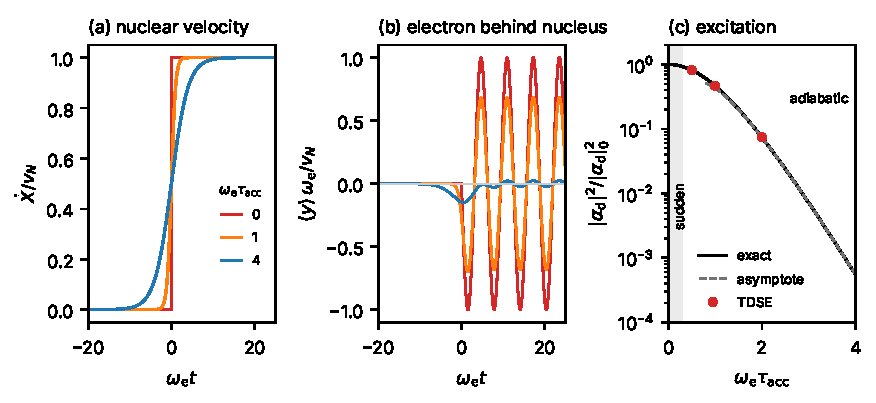
\includegraphics[width=\linewidth]{figures/ch06/fig6_1.pdf}
  \caption{Adiabatic and sudden responses of an electron to a moving nucleus, in a model in which one electron is bound to the nucleus by a harmonic force of frequency $\omega_{\mathrm{e}}$ and the nucleus follows a prescribed classical path. (a) The velocity of the nucleus, $\dot X = \tfrac12v_N[1 + \tanh(t/\tau_{\mathrm{acc}})]$, for acceleration times $\omega_{\mathrm{e}}\tau_{\mathrm{acc}} = 0$ (an instantaneous kick), 1 and 4. (b) The mean position $\langle y\rangle$ of the electron relative to the nucleus, in units of $v_N/\omega_{\mathrm{e}}$, for the same three cases. After a kick the electron oscillates about the nucleus with the full amplitude; after a slow acceleration it lags behind while the force acts and returns to rest. (c) The excitation $|\alpha_{\mathrm{d}}|^2 = -\ln P_0$, with $P_0$ the probability that the electron ends in the ground state, divided by its value $|\alpha_{\mathrm{d}}|^2_0 = m_ev_N^2/2\omega_{\mathrm{e}}$ for an instantaneous kick, against $\omega_{\mathrm{e}}\tau_{\mathrm{acc}}$. Solid: the exact result \cref{eq:6.1-model}. Dashed: its adiabatic asymptote $\pi^2(\omega_{\mathrm{e}}\tau_{\mathrm{acc}})^2\ee^{-\pi\omega_{\mathrm{e}}\tau_{\mathrm{acc}}}$. Dots: $-\ln P_0$ from a split-operator solution of the time-dependent Schr\"odinger equation for $m_ev_N^2/2\omega_{\mathrm{e}} = 1/2$. Shaded: the sudden region $\omega_{\mathrm{e}}\tau_{\mathrm{acc}} < 0.3$, where the excitation is within \SI{10}{\percent} of its sudden value.}
  \label{fig:6-sudden}
\end{figure}

For a nucleus in a crystal two times matter: how long the kick lasts, and how soon the neighbors start pulling the nucleus back. The kick itself is fast. A classical estimate of its duration, a heuristic only, is the time the dark matter takes to cross the region where it interacts with the nucleus. For a contact interaction and a silicon nucleus of radius \SI{3.5}{fm} this is $\SI{4e-21}{s}$ at $v_{\mathrm{max}}$, while $1/\Eg = \SI{0.56}{fs}$. The deceleration is slow. After the kick the nucleus is pulled back by the lattice over a time $\sim1/\omega_{\mathrm{ph}}$, which is the adiabatic regime for every excitation across the gap. In the model, take a nucleus that is kicked at $t = 0$ and then oscillates at $\omega_{\mathrm{ph}}$ in a harmonic well, $X(t) = (v_N/\omega_{\mathrm{ph}})\sin\omega_{\mathrm{ph}}t$ for $t > 0$. Its acceleration is $\ddot X = v_N\delta(t) - v_N\omega_{\mathrm{ph}}\sin(\omega_{\mathrm{ph}}t)\,\Theta(t)$, and $\int\dd t\,\ddot X\,\ee^{\ii\omega_{\mathrm{e}}t} = v_N/[1 - (\omega_{\mathrm{ph}}/\omega_{\mathrm{e}})^2]$, so $|\alpha_{\mathrm{d}}|^2$ exceeds the free-recoil value by the factor $[1 - (\omega_{\mathrm{ph}}/\omega_{\mathrm{e}})^2]^{-2}$. With $\omega_{\mathrm{ph}}/\omega_{\mathrm{e}}$ set to the ratio $\omega_{\mathrm{opt}}/\Eg = 0.055$ of the zone-center optical phonon of silicon, $\omega_{\mathrm{opt}} = \SI{64.1}{meV}$, to its gap, the factor is 1.006. A kicked nucleus in an insulator therefore excites its electrons as if it were free, with corrections of relative order $(\omega_{\mathrm{ph}}/\Delta E)^2$, the square of the small ratio that controls the adiabatic approximation. The sudden picture fails where that ratio is not small, for excitation energies comparable to phonon energies, as at the Fermi surface of a metal, and where the classical path itself fails, for recoil energies $q^2/2M$ that do not exceed a phonon energy (\cref{sec:5.6}). There the nucleus does not recoil, the kick creates a few phonons, and the electron--lattice response of \cref{sec:12.1} replaces the trajectory.

\subsection{The sudden kick}

In the sudden limit the result does not need perturbation theory. Immediately after the kick the electronic wavefunction is what it was before, $\Psi_0(r;u)$, but the nucleus moves with velocity $\vect{v}_N$. In the frame that moves with the nucleus, the electrons have all acquired the velocity $-\vect{v}_N$. A Galilean boost of every electron by $-\vect{v}_N$ multiplies the wavefunction by a plane wave:
\begin{equation}
  \Psi_0 \;\to\; \exp\Bigl(-\ii m_e\vect{v}_N\cdot\sum_e(\vect{r}_e - \vect{X})\Bigr)\Psi_0 , \qquad
  P_0 = \Bigl|\Bigl\langle\Psi_0\Bigr|\exp\Bigl(-\ii m_e\vect{v}_N\cdot\sum_e\vect{r}_e\Bigr)\Bigl|\Psi_0\Bigr\rangle\Bigr|^2 ,
  \label{eq:6.1-boost}
\end{equation}
where in $P_0$, the probability that the electrons are found in the ground state around the moving nucleus, the phase $\ee^{\ii m_e\vect{v}_N\cdot\vect{X}}$ drops out. This is Migdal's formulation~\cites{migdal1941ionization}[Eqs.~(1) and~(2)]{ibe2018migdal}. To first order in $v_N$ the amplitude of an excited state is $-\ii m_e\vect{v}_N\cdot\langle\Psi_j|\sum_e\vect{r}_e|\Psi_0\rangle$, a dipole transition driven by the kick. It agrees with \cref{eq:6.1-sudden1}. For an atom the adiabatic states depend on the nuclear position only through $\vect{r}_e - \vect{X}$, so that $\nabla_{\vect{X}}\Psi_0 = -\sum_e\nabla_e\Psi_0$, and the total electron momentum is $-\ii\sum_e\nabla_e = \ii m_e[H_{\mathrm{el}}, \sum_e\vect{r}_e]$. Taking the matrix element between $\Psi_j$ and $\Psi_0$, $\vect{d}_{j0} = m_e\Delta E_j\,\langle\Psi_j|\sum_e\vect{r}_e|\Psi_0\rangle$, and \cref{eq:6.1-sudden1} becomes the dipole amplitude. The derivative coupling of an atom is its dipole matrix element times the excitation energy and the electron mass.

For one electron in hydrogen the sudden result is exact. The Hamiltonian $p_e^2/2m_e + p_p^2/2m_p - \alpha/|\vect{r}_e - \vect{X}|$ separates into the motion of the center of mass $\vect{R}_{\mathrm{cm}} = (m_p\vect{X} + m_e\vect{r}_e)/M_{\mathrm{H}}$, with $M_{\mathrm{H}} = m_p + m_e$, and the relative coordinate $\vect{\rho} = \vect{r}_e - \vect{X}$, whose ground state is the 1s state with the reduced mass $\mu_{ep} = m_em_p/M_{\mathrm{H}}$ and the Bohr radius $a_{ep} = 1/(\alpha\mu_{ep})$. Dark matter that couples to the proton acts on the atom, to first order in its coupling, through $\ee^{\ii\vect{q}\cdot\vect{X}}$ (\cref{sec:2.2}); a coupling of the dark matter to the electron itself is a separate process, which we leave aside. Since $\vect{X} = \vect{R}_{\mathrm{cm}} - (m_e/M_{\mathrm{H}})\vect{\rho}$,
\begin{equation*}
  \ee^{\ii\vect{q}\cdot\vect{X}} = \ee^{\ii\vect{q}\cdot\vect{R}_{\mathrm{cm}}}\;\ee^{-\ii(m_e/M_{\mathrm{H}})\vect{q}\cdot\vect{\rho}} .
\end{equation*}
The first factor gives the whole atom the momentum $\vect{q}$. The second acts on the internal state like a momentum transfer $-(m_e/M_{\mathrm{H}})\vect{q}$ to the electron, and its ground-state expectation value is the elastic form factor \cref{eq:2.2-F1s} with $a_{ep}$ in place of $a_0$. Its argument is $(m_eq/M_{\mathrm{H}})\,a_{ep} = q/(\alpha m_p) = v_N/\alpha$, where $v_N = q/m_p$ is the velocity given to the proton, and the reduced-mass corrections cancel. With $a_0 = 1/(\alpha m_e)$ we may write the argument as $m_ev_Na_0$:
\begin{keyresult}[Sudden kick of a hydrogen atom]
A hydrogen atom in its ground state whose nucleus is given the velocity $v_N = q/m_p$ remains in its ground state with probability
\begin{equation}
  P_0 = \bigl|F_{1s}(m_ev_N)\bigr|^2 = \left[\frac{16}{(4 + v_N^2/\alpha^2)^2}\right]^2 \simeq 1 - \frac{v_N^2}{\alpha^2} \quad (v_N \ll \alpha) ,
  \label{eq:6.1-P0}
\end{equation}
and is excited or ionized with probability $1 - P_0$. The controlling ratio is that of the nuclear velocity to the orbital velocity $\alpha$ of the electron.
\end{keyresult}
The derivation used no assumption about time. In a first-order amplitude the momentum transfer is a single act, and the dark matter couples to the nuclear coordinate only. Nothing in a free atom decelerates the nucleus afterward, and the separation of the center of mass does the work that suddenness did in \cref{eq:6.1-boost}. Ibe et al.\ derive the general atom in this way, with the amplitude of every electronic transition given by \cref{eq:6.1-boost} and the energy of the atom conserved overall~\cite[Eqs.~(55)--(58)]{ibe2018migdal}. For more than one electron the separation is not exact, and the argument $m_ev_N$ is corrected at relative order $m_e/M$; \cref{sec:12.2} makes this precise.

The fraction $1 - P_0$ of nuclear recoils that leave the atom excited or ionized is the \emph{Migdal effect}. Its interest for dark-matter searches is the energy it adds. A recoil of a few hundred eV in silicon may be below the threshold of a phonon or charge readout. An electron--hole pair from the same event, carrying at least the gap, is easy to count. In a crystal the electrons are shared between atoms, and the excitation is an electron--hole pair rather than an atomic transition.

\begin{workedexample}{Ground-state survival of a kicked hydrogen atom}\label{we:6-hydrogen}
Dark matter of $\mchi = \SI{1}{GeV}$ scatters elastically off a hydrogen atom at rest, at the largest laboratory speed $v_{\mathrm{max}} = 2.650\times10^{-3}$ (\cref{eq:1.2-vmax}). The atom has the mass $M_{\mathrm{H}} = \SI{938.783}{MeV}$, the reduced mass is $\mu_{\chi\mathrm{H}} = (1000 \times 938.783/1938.783)\,\si{MeV} = \SI{484.2}{MeV}$, and the largest momentum transfer is $q = 2\mu_{\chi\mathrm{H}}v_{\mathrm{max}} = \SI{2.566}{MeV}$, at which the atom recoils with $q^2/2M_{\mathrm{H}} = \SI{3.51}{keV}$.

The proton, of mass $m_p = \SI{938.272}{MeV}$, is kicked to $v_N = q/m_p = 2.735\times10^{-3}$, or \SI{820}{km.s^{-1}}; dark matter as heavy as the target bounces it at about its own speed. In units of the orbital velocity, $v_N/\alpha = 0.375$. Then $F_{1s}(m_ev_N) = 16/(4 + 0.1405)^2 = 0.933$, and \cref{eq:6.1-P0} gives
\begin{equation*}
  P_0 = 0.871 , \qquad 1 - P_0 = 0.129 .
\end{equation*}
One such recoil in eight leaves the atom excited or ionized, with at least the \SI{10.2}{eV} of the $1s \to 2p$ transition in its electrons. The small-$v_N$ form, $v_N^2/\alpha^2 = 0.140$, is \SI{9}{\percent} high at this velocity. The atom survives with probability one half at $v_N/\alpha = 0.87$, where $F_{1s}^2 = \tfrac12$ (\cref{we:2-hydrogen}): $v_N = 6.35\times10^{-3}$, $q = \SI{5.96}{MeV}$ and a recoil of \SI{18.9}{keV}, beyond the reach of dark matter at this mass.

Is the kick sudden? The excitation energies start at $\Delta E = \tfrac38\alpha^2m_e = \SI{10.2}{eV}$, so the electron responds on the time $1/\Delta E = \SI{0.065}{fs}$. Dark matter with a contact interaction crosses the proton, of charge radius \SI{0.84}{fm}~\cite{mohr2025codata}, in $\SI{1.1e-21}{s}$, and $\Delta E\,\tau_{\mathrm{acc}} = 1.6\times10^{-5}$: on the scale of \cref{fig:6-sudden}(c) the kick is instantaneous.

For the kick of the opening, $v_N = 1.95\times10^{-4}$ for a silicon nucleus, the same formula gives $1 - P_0 = 7.1\times10^{-4}$ for an electron bound as in hydrogen. The outer electrons of silicon are bound more weakly and the inner ones far more strongly, so this is an order-of-magnitude statement.
\end{workedexample}

\section{Electron--phonon matrix elements}\label{sec:6.2}

An electron at the bottom of the conduction band of GaAs absorbs a longitudinal optical phonon of wavevector \SI{0.01}{\angstrom^{-1}} with a vertex $|g| = \SI{3.3}{eV}$. An electron in a conduction valley of silicon absorbs a longitudinal sound wave of the same wavevector, running along the valley axis, with $|g| = \SI{26}{meV}$, more than a hundred times less. Ten times longer wavelengths make the GaAs vertex ten times larger and the silicon one $\sqrt{10}$ times smaller. Both numbers follow from the definition \cref{eq:6.1-Hep} once the bare potential of a displaced nucleus is replaced by the potential that the electrons actually feel, screened by all the other electrons. The coupling to long-wavelength sound waves controls how an excited carrier in silicon sheds its last few meV. The Fr\"ohlich coupling of GaAs is the electron's view of the same macroscopic field through which a dark photon drives the optical phonons of a polar crystal (\cref{sec:5.5}). The phonon that lets a slow dark-matter particle cross the indirect gap of silicon enters through the same vertex, at large wavevector (\cref{sec:6.5}).

\subsection{The screened vertex}

The bare potential of a displaced nucleus is long-ranged. A pseudo-ion of valence charge $Z_\kappa$ has the potential energy $v_\kappa(k) \to -Z_\kappa e^2/k^2$ for an electron at small wavevector $k$, the Coulomb tail of \cref{eq:A.2-vC}. Its gradient, the force field of \cref{sec:6.1}, has the Fourier components $-\ii\vect{k}\,v_\kappa(k)$. A displacement wave of wavevector $\vect{Q}$ therefore has a bare potential whose component at $\vect{Q}$ grows as $Z_\kappa e^2/Q$, for every crystal. The electrons undo most of this. They flow toward a displaced positive ion and away from the region it left, and what an electron near the ion feels is the change of the self-consistent potential, $\partial_{\kappa\alpha,\vect{Q}}V_{\mathrm{KS}}$ of \cref{eq:5.4-dV}, not the change of the bare one.

The screening can be written in one line. The first-order density of \cref{eq:5.4-dn} is the static Kohn--Sham response to the screened potential, $\partial\nd = R^0\,\partial V_{\mathrm{KS}}$, with $R^0$ the independent-particle response of \cref{sec:4.6} at $\omega = 0$, and \cref{eq:5.4-dV} adds back the Hartree and exchange--correlation potentials of that density, $\partial V_{\mathrm{KS}} = \partial V_{\mathrm{ext}} + f_{\mathrm{Hxc}}\,\partial\nd$ with $f_{\mathrm{Hxc}} = v_{\mathrm{C}} + f_{\mathrm{xc}}$. Eliminating $\partial\nd$,
\begin{equation}
  \partial_{\kappa\alpha,\vect{Q}}V_{\mathrm{KS}} = \bigl(1 - f_{\mathrm{Hxc}}R^0\bigr)^{-1}\,\partial_{\kappa\alpha,\vect{Q}}V_{\mathrm{ext}}
  = \bigl(1 + f_{\mathrm{Hxc}}R\bigr)\,\partial_{\kappa\alpha,\vect{Q}}V_{\mathrm{ext}} ,
  \label{eq:6.2-screen}
\end{equation}
where products are integral operators in space, or matrices in the reciprocal-lattice vectors $\vect{Q}+\vect{G}$ at fixed $\vect{Q}$, and $R = R^0(1 - f_{\mathrm{Hxc}}R^0)^{-1}$ is the full static response of \cref{eq:4.6-tddft}; the form with $1 + f_{\mathrm{Hxc}}R$ follows from expanding the inverse in powers of $f_{\mathrm{Hxc}}R^0$. With $f_{\mathrm{xc}}$ dropped, $1 + v_{\mathrm{C}}R$ is the inverse dielectric matrix $\varepsilon^{-1}_{\vect{G}\vect{G}'}(\vect{Q},0)$ of \cref{eq:4.4-epsGG}. With it, the operator is the inverse dielectric function of a \emph{test electron}: the potential that a second electron feels includes the exchange--correlation hole that the response builds around it, while the test charge of \cref{sec:4.4} feels only the Hartree part. The screening is static. A phonon of tens of meV is slow compared with the electronic response of an insulator, whose scale is the gap, and the static limit is the adiabatic approximation of \cref{sec:6.1}. Below the gap a response function is even in the frequency, so the static screening is accurate to relative order $(\omega_{\mathrm{ph}}/\Eg)^2$, as are the phonon frequencies (\cref{sec:6.4}). The first power of $\omega_{\mathrm{ph}}/\Eg$ in \cref{sec:6.1} measures the amplitude for exciting the electrons, not the change of their response. Screening of the ionic potential by the static Lindhard function goes back to Bardeen, as quoted by Giustino~\cite[Eqs.~(3)--(5)]{giustino2017electron}. In a metal, whose response has no gap, the same structure appears with the response evaluated at the phonon frequency, the dynamically screened vertex of Bardeen and Pines~\cite{bardeen1955electron}.

How much is left at long wavelength depends on the material. In a metal, the Thomas--Fermi limit of \cref{eq:4.4-TF} divides the bare $Z_\kappa e^2/Q$ by $\varepsilon_{\mathrm{TF}}(Q) = 1 + k_{\mathrm{TF}}^2/Q^2$, and the screened vertex becomes $Z_\kappa e^2Q/(Q^2 + k_{\mathrm{TF}}^2)$: the divergence has turned into a coupling that vanishes linearly in $Q$. The electrons have neutralized the displaced ion completely. In an insulator the head of the dielectric matrix tends to $\varepsilon_\infty$, which reduces the bare $1/Q$ tail by a factor of 11.7 in silicon but does not remove it. The tail is removed by the local fields of \cref{sec:4.4}, the off-diagonal elements $\varepsilon^{-1}_{\vect{0}\vect{G}}$ that describe electrons moving with the ion on the scale of a bond. Their effect is to replace the ionic charge by the Born effective charge of \cref{sec:5.5}. A displaced ion drags part of its bond charge along, and the induced density at the wavevectors $\vect{Q} + \vect{G}$ with $\vect{G} \ne 0$ is this comoving cloud. Its dipole per unit displacement is $-e(Z_\kappa - Z^*_\kappa)$, so that ion and cloud together carry $eZ^*_\kappa$. At long wavelength a displaced, screened ion is a dipole $eZ^*_\kappa\cdot\vect{u}$ in a medium of dielectric constant $\varepsilon_\infty$, as Pick, Cohen and Martin showed from the structure of the dielectric matrix~\cite{pick1970microscopic}. In silicon $Z^* = 0$. The electron cloud follows each nucleus so well that no dipole is left, and the long-range part of the screened potential starts at the quadrupole. In GaAs $Z^* = 2.1$, the dipole survives, and its field gives the $1/Q$ vertex of the opening, the Fr\"ohlich coupling.

\Cref{eq:6.1-Hep} with the screened potential is the vertex that density-functional perturbation theory computes. Since $\partial_{\kappa\alpha,\vect{Q}}V_{\mathrm{KS}}$ is a Bloch function of crystal momentum $\vect{Q}$, we write it as $\ee^{\ii\vect{Q}\cdot\vect{r}}\,\partial_{\kappa\alpha,\vect{Q}}v_{\mathrm{KS}}(\vect{r})$, with $\partial_{\kappa\alpha,\vect{Q}}v_{\mathrm{KS}}$ periodic in the lattice. With the Bloch states of \cref{eq:A.5-bloch}, the phases $\ee^{-\ii(\vect{k}+\vect{Q})\cdot\vect{r}}\ee^{\ii\vect{Q}\cdot\vect{r}}\ee^{\ii\vect{k}\cdot\vect{r}}$ cancel, as they did for the density vertex \cref{eq:A.5-rho}, the factor $1/N$ cancels the $N$ cells, and
\begin{equation}
  g_{mn\nu}(\vect{k},\vect{Q}) = \ell_{\vect{Q}\nu}\,\bigl\langle u_{m,\vect{k}+\vect{Q}}\bigr|\,\Delta_{\vect{Q}\nu}v_{\mathrm{KS}}\,\bigl|u_{n\vect{k}}\bigr\rangle_\Omega ,
  \qquad
  \Delta_{\vect{Q}\nu}v_{\mathrm{KS}} = \sum_{\kappa\alpha}\Bigl(\frac{M_{\mathrm{cell}}}{M_\kappa}\Bigr)^{1/2}e^\alpha_{\kappa\nu}(\vect{Q})\;\partial_{\kappa\alpha,\vect{Q}}v_{\mathrm{KS}} ,
  \label{eq:6.2-g}
\end{equation}
where the bracket is an integral over one cell. We have written the prefactor $(2M_\kappa\omega_{\vect{Q}\nu})^{-1/2}$ of \cref{eq:A.6-g} as the zero-point length $\ell_{\vect{Q}\nu}$ of \cref{eq:A.6-ell} times $(M_{\mathrm{cell}}/M_\kappa)^{1/2}$. This is the normalization of Refs.~\cite[Eqs.~(33)--(38)]{giustino2017electron} and~\cite[Eq.~(2)]{ponce2016epw}. The zero-point length, typically a few hundredths of an \si{\angstrom} for an optical phonon, carries all the mass and frequency dependence. What is left is how much the potential changes when the atoms move, the matrix element of $\Delta_{\vect{Q}\nu}v_{\mathrm{KS}}$ per unit mass-weighted displacement, in eV per \si{\angstrom}. For an acoustic mode at small $Q$, where $(M_{\mathrm{cell}}/M_\kappa)^{1/2}\vect{e}_{\kappa\nu} = \hat{\vect{e}}_\nu$ for every $\kappa$ (\cref{sec:5.3}), it is the potential change per unit displacement of the whole crystal. The vertex itself has the dimension of energy, and $|g|^2/N$ is the squared amplitude per mode. The vertex depends on the phases of the two Bloch states, as $\rho_{mn}$ does in \cref{eq:A.5-gauge}; only sums of $|g|^2$ over degenerate partners can be compared between calculations.

In practice one run of density-functional perturbation theory per phonon wavevector solves the Sternheimer equation \cref{eq:5.4-sth} for the three displacement directions of every atom and returns $\partial_{\kappa\alpha,\vect{Q}}v_{\mathrm{KS}}$ together with the phonon frequencies and polarization vectors. The vertex for any pair of bands and any $\vect{k}$ then costs just one matrix element, \cref{eq:6.2-g}, one application of a known potential to a known state. The run does not change for the vertex: the screened potential is the quantity whose self-consistency already produced the phonon. \Cref{app:E.4} describes such a run and its convergence parameters, and \cref{app:E.5} the step from a coarse set of such vertices to the dense grids of a rate, whose principle closes this section.

\subsection{Acoustic phonons and deformation potentials}

Moving the whole crystal changes no band energy. If every nucleus is displaced by the same vector $\vect{t}$ and the electrons follow, the self-consistent potential is translated with them, $V_{\mathrm{KS}}(\vect{r};u + t) = V_{\mathrm{KS}}(\vect{r} - \vect{t};u)$, or $\op{T}_{\vect{t}}V_{\mathrm{KS}}\op{T}^\dagger_{\vect{t}}$ with the translation operator $\op{T}_{\vect{t}} = \ee^{-\ii\vect{t}\cdot\op{\vect{p}}}$ when the potential is a nonlocal pseudopotential. Differentiating at $\vect{t} = 0$ collects the derivatives with respect to all nuclei into the derivative of the potential with respect to the electron coordinate. The sum over all cells and all species is the displacement wave at $\vect{Q} = 0$ summed over $\kappa$, so $\sum_\kappa\partial_{\kappa\alpha,\vect{0}}V_{\mathrm{KS}} = -\ii[\op{p}_\alpha, V_{\mathrm{KS}}] = -\ii[\op{p}_\alpha, H_{\mathrm{KS}}]$, where the last step uses that the kinetic energy commutes with the momentum. Between two Bloch states at the same $\vect{k}$, eigenstates of $H_{\mathrm{KS}}$,
\begin{equation}
  \sum_\kappa\bigl\langle\psi_{m\vect{k}}\bigr|\,\partial_{\kappa\alpha,\vect{0}}V_{\mathrm{KS}}\,\bigl|\psi_{n\vect{k}}\bigr\rangle
  = -\ii\,(\varepsilon_{n\vect{k}} - \varepsilon_{m\vect{k}})\,p^\alpha_{mn}(\vect{k}) ,
  \label{eq:6.2-asr}
\end{equation}
with $p^\alpha_{mn}$ the momentum matrix element of \cref{sec:3.2}. The diagonal element vanishes: a rigid translation does not shift band $n$ at first order. This is the acoustic sum rule of the vertex, the counterpart of \cref{eq:5.2-asr} for the force constants, and like it, it follows from translation invariance alone.

An acoustic phonon at small $Q$ approaches this rigid translation. Its polarization vectors tend to $(M_\kappa/M_{\mathrm{cell}})^{1/2}\hat{\vect{e}}_\nu$ (\cref{sec:5.3}), so that $\Delta_{\vect{Q}\nu}v_{\mathrm{KS}}$ in \cref{eq:6.2-g} becomes $\hat{\vect{e}}_\nu\cdot\sum_\kappa\partial_{\kappa,\vect{Q}}v_{\mathrm{KS}}$, and \cref{eq:6.2-asr} makes its diagonal matrix element vanish as $Q \to 0$. What survives is the next order in $Q$, multiplied by a zero-point length that grows as $\ell_{\vect{Q}\nu} = (2M_{\mathrm{cell}}c_\nu Q)^{-1/2}$. The intraband vertex therefore vanishes as
\begin{equation*}
  g_{nn\nu}(\vect{k},\vect{Q}) \propto Q\,\ell_{\vect{Q}\nu} \propto Q^{1/2} \qquad (\nu \text{ acoustic},\ Q \to 0) ,
\end{equation*}
the statement that $g_{nn\nu}(\vect{k},\vect{0}) = 0$ for acoustic modes. The interband elements of \cref{eq:6.2-asr} do not vanish. They describe the rigid translation of the electronic state itself: shifted by $\ell_{\vect{Q}\nu}\hat{\vect{e}}_\nu$, a state changes by $-\ell_{\vect{Q}\nu}\hat{\vect{e}}_\nu\cdot\nabla\psi_{n\vect{k}}$, which written in the other bands at the same $\vect{k}$ is exactly this matrix element divided by $\varepsilon_{n\vect{k}} - \varepsilon_{m\vect{k}}$. No energy is exchanged in such a change, and in the energy shifts of \cref{sec:6.3} it cancels against the second-order Allen--Heine term, as translation invariance demands. Codes therefore set the vertices of the three acoustic modes at $\vect{Q} = 0$ to zero~\cite[below Eq.~(38)]{giustino2017electron}.

The term of first order in $Q$ is the deformation potential. Consider a region short compared with the wavelength $2\pi/Q$ but containing many cells. There one long acoustic mode displaces every nucleus by the same amount, $\vect{u}(\vect{r}) = (\ell_{\vect{Q}\nu}/\sqrt N)\,\hat{\vect{e}}_\nu\,\ee^{\ii\vect{Q}\cdot\vect{r}}B_{\vect{Q}\nu}$, and the crystal is locally translated and uniformly strained, with strain tensor
\begin{equation*}
  S_{\alpha\beta}(\vect{r}) = \tfrac12\bigl(\partial_\alpha u_\beta + \partial_\beta u_\alpha\bigr) = \frac{\ii}{2}\bigl(Q_\alpha\hat e_{\nu\beta} + Q_\beta\hat e_{\nu\alpha}\bigr)\,\frac{\ell_{\vect{Q}\nu}}{\sqrt N}\,\ee^{\ii\vect{Q}\cdot\vect{r}}B_{\vect{Q}\nu} .
\end{equation*}
The translation does nothing, by \cref{eq:6.2-asr}. A uniform strain shifts the band energies at first order, $\delta\varepsilon_{n\vect{k}} = \sum_{\alpha\beta}D^n_{\alpha\beta}S_{\alpha\beta}$, and this defines the \emph{deformation-potential tensor} $D^n_{\alpha\beta}$ of band $n$ near the extremum of interest. It is symmetric, and it is taken with the nuclei inside each cell relaxed, since a long acoustic wave carries the internal relaxation of \cref{sec:5.2} with it. An electron near the band edge, in a wavepacket much longer than the cell but short compared with $2\pi/Q$, feels the slowly varying shift $\delta\varepsilon_n(\vect{r})$ as a potential energy. This is the argument of Bardeen and Shockley~\cite{bardeen1950deformation}. The matrix element of that potential between $n\vect{k}$ and $n,\vect{k}+\vect{Q}$ is the amplitude of the shift times $\rho_{nn}(\vect{k},\vect{Q}) \simeq 1$. Comparison with \cref{eq:6.1-Hep} gives
\begin{equation}
  g_{nn\nu}(\vect{k},\vect{Q}) = \ii\,\ell_{\vect{Q}\nu}\sum_{\alpha\beta}Q_\alpha D^n_{\alpha\beta}\,\hat e_{\nu\beta} \qquad (\nu \text{ acoustic},\ Q \to 0) .
  \label{eq:6.2-D}
\end{equation}
For a band extremum at $\mathrm{\Gamma}$ in a cubic crystal the tensor is a multiple of the identity, $D^n_{\alpha\beta} = E_1\delta_{\alpha\beta}$, and $E_1 = \Omega\,\partial\varepsilon_n/\partial\Omega$, since the trace of the strain is the relative change of volume~\cite[Eq.~(6)]{giustino2017electron}. Only the longitudinal mode couples, through $\vect{Q}\cdot\hat{\vect{e}}_\nu$: a transverse wave shears the crystal without changing its volume. With $\omega_{\vect{Q}\nu} = c_{\mathrm{LA}}Q$, $|g|^2 = E_1^2Q/(2M_{\mathrm{cell}}c_{\mathrm{LA}})$. Bardeen and Shockley obtained $E_1$ for the band edges of silicon by fitting measured mobilities to this form~\cite{bardeen1950deformation}.

The conduction valleys of silicon are not at $\mathrm{\Gamma}$. Each is symmetric only about its own axis $\hat{\vect{k}}_{\mathrm{c}}$ (\cref{sec:3.3}), and the most general symmetric tensor with that symmetry has two constants, $D_{\alpha\beta} = \Xi_d\,\delta_{\alpha\beta} + \Xi_u\,\hat k_{\mathrm{c}\alpha}\hat k_{\mathrm{c}\beta}$, the dilatation and uniaxial deformation potentials of Herring and Vogt~\cite{herring1956transport}. With $\theta$ the angle between $\vect{Q}$ and the valley axis, \cref{eq:6.2-D} gives the effective constants $\Xi_d + \Xi_u\cos^2\theta$ for the longitudinal mode and $\Xi_u\sin\theta\cos\theta$ for the transverse mode polarized in the plane of $\vect{Q}$ and $\hat{\vect{k}}_{\mathrm{c}}$; the other transverse mode does not couple~\cite[Eqs.~(13) and (14)]{li2021deformation}. Li, Graziosi and Neophytou extracted the two constants from the slopes of DFPT vertices of silicon at small $Q$, and found $\Xi_d = \SI{1.01}{eV}$ and $\Xi_u = \SI{8.84}{eV}$~\cite{li2021deformation}. A longitudinal phonon of $Q = \SI{0.01}{\angstrom^{-1}}$ along the valley axis has \SI{0.55}{meV} and a zero-point length $\ell_{\vect{Q}\nu} = \SI{0.26}{\angstrom}$, and \cref{eq:6.2-D} yields $|g| = 9.85\times0.01\times\SI{0.26}{eV} = \SI{26}{meV}$, the number of the opening. Across the valley axis the coupling is almost ten times weaker, \SI{2.6}{meV}. \Cref{fig:6-gQ} shows both against $Q$. The form holds for intraband scattering near a band edge, for $Q$ small compared with the zone; the computed matrix elements are linear in $Q$ over the whole computed range, up to \SI{0.1}{\angstrom^{-1}}~\cite[Fig.~5]{li2021deformation}.

In a crystal without inversion symmetry, such as GaAs, a strain also polarizes the cell, $P_\alpha = \sum_{\beta\gamma}e^{\mathrm{pz}}_{\alpha\beta\gamma}S_{\beta\gamma}$ with the piezoelectric tensor $e^{\mathrm{pz}}$, and an acoustic wave then carries a macroscopic field. The steps of \cref{app:D.14} that turn the polarization of a longitudinal optical wave into the Fr\"ohlich vertex apply unchanged. The field obeys $\hat{\vect{Q}}\cdot(\varepsilon_\infty\vect{\mathcal{E}} + \vect{P}) = 0$, an electron feels the potential energy $V = e\hat{\vect{Q}}\cdot\vect{\mathcal{E}}/(\ii Q)$, and with the strain above
\begin{equation*}
  g^{\mathrm{pz}}_{mn\nu}(\vect{k},\vect{Q}) = -\frac{e}{\varepsilon_\infty}\,\ell_{\vect{Q}\nu}\sum_{\alpha\beta\gamma}\hat Q_\alpha\,e^{\mathrm{pz}}_{\alpha\beta\gamma}\,\hat Q_\beta\,\hat e_{\nu\gamma}\;\rho_{mn}(\vect{k},\vect{Q}) ,
\end{equation*}
for a cubic crystal. This is the \emph{piezoelectric coupling}. The factor $Q$ of the strain cancels the $1/Q$ of the field, and the vertex depends on $Q$ only through $\ell_{\vect{Q}\nu} \propto Q^{-1/2}$ and on the direction of $\vect{Q}$. It grows at long wavelength, more gently than the Fr\"ohlich vertex. In a first-principles calculation it comes from two terms. One is the dynamical quadrupoles of the displaced atoms, the next term after the Born charge in the long-wavelength expansion of the charge that a displaced atom induces. The other is the Born charges of the relative sublattice displacement that the strain induces. In GaAs it dominates the scattering of electrons by acoustic phonons~\cite{brunin2020electron}; \cref{app:E.5} treats it with the other long-range terms.

\subsection{Optical deformation potential}

An optical phonon at $\vect{Q} = 0$ moves the sublattices against each other. Nothing in the translation argument forces its vertex to vanish, and in general it does not: bond lengths and angles inside the cell change at first order in the displacement, and so do the band energies. The vertex is finite at $\vect{Q} = 0$, and it is conventionally written as
\begin{equation}
  g_{nn\nu}(\vect{k},\vect{0}) = \ell_{\vect{0}\nu}\,d^n_\nu , \qquad
  d^n_\nu = \bigl\langle\psi_{n\vect{k}}\bigr|\sum_{\kappa}\Bigl(\frac{M_{\mathrm{cell}}}{M_\kappa}\Bigr)^{1/2}\vect{e}_{\kappa\nu}(\vect{0})\cdot\partial_{\kappa,\vect{0}}V_{\mathrm{KS}}\bigl|\psi_{n\vect{k}}\bigr\rangle ,
  \label{eq:6.2-d}
\end{equation}
with $d^n_\nu$ the \emph{optical deformation potential} of band $n$, in eV per \si{\angstrom}. Since $\partial_{\kappa,\vect{0}}V_{\mathrm{KS}}$ displaces a whole sublattice, $d^n_\nu$ is, by the Hellmann--Feynman theorem of \cref{sec:5.1}, the shift of $\varepsilon_{n\vect{k}}$ per unit mass-weighted displacement of the sublattices in the pattern of mode $\nu$. In silicon the two atoms have equal masses, $\vect{e}_{1\nu} = -\vect{e}_{2\nu} = \hat{\vect{e}}/\sqrt2$, and the pattern moves the two atoms of every cell by $+u\hat{\vect{e}}$ and $-u\hat{\vect{e}}$; $d^n_\nu$ is then $\dd\varepsilon_{n\vect{k}}/\dd u$. Compared with the acoustic constant $D^n$, which enters with an extra factor $Q$, $d^n_\nu$ is of zeroth order in $Q$, and the two are often called the first-order and zero-order deformation potentials.

Symmetry can still make $d^n_\nu$ vanish, and for the conduction valleys of silicon it does: within a valley the electrons scatter off acoustic phonons only, and DFPT finds the intravalley optical vertices small near $\vect{Q} = 0$~\cite{li2021deformation}. The valence maximum is threefold degenerate at $\mathrm{\Gamma}$ (\cref{sec:3.3}), and the optical phonon splits it. For a degenerate level the coupling is a matrix in the partners; Li et al.\ combine its elements into a single value, \SI{10.45}{eV.\angstrom^{-1}}, the mean of two such combinations~\cite[Eq.~(12) and the text below it]{li2021deformation}. With $\omega_{\vect{0}\nu} = \SI{64.1}{meV}$ the zero-point length of the optical mode is $\ell_{\vect{0}\nu} = \SI{0.024}{\angstrom}$. That is half the \SI{0.048}{\angstrom} of the bond coordinate in \cref{sec:5.1}, because $\ell$ refers the motion to the mass of the whole cell, and the vertex of the holes is $|g| \simeq \SI{0.25}{eV}$, independent of $Q$ near the zone center (\cref{fig:6-gQ}). It is ten times the acoustic vertex of the electrons at $Q = \SI{0.01}{\angstrom^{-1}}$, but the phonon it emits costs \SI{64}{meV}, which a hole near the band edge does not have. Electrons in silicon meet the same zero-order coupling when they scatter between valleys. The crystal momentum between two valleys is a sizable fraction of the zone, the phonons that supply it are near the zone boundary, and the vertex is finite there; such intervalley processes cool hot carriers in a detector (\cref{app:E.12}). In a polar crystal the optical deformation potential is present as well, but the longitudinal optical mode carries in addition the macroscopic field.

\subsection{The Fr\"ohlich vertex}

In a longitudinal optical wave of GaAs the gallium and arsenic sublattices move against each other along $\vect{Q}$, every cell acquires a dipole $eZ^*\vect{u}_{\mathrm{rel}}$, with $\vect{u}_{\mathrm{rel}} = \vect{u}_1 - \vect{u}_2$ the relative displacement of the two sublattices (\cref{app:D.14}), and the dipoles of a long wave add up to a macroscopic polarization. Its field reaches every electron in the crystal, however far from the displaced atoms. \Cref{app:D.14} computes that field from the condition $\hat{\vect{Q}}\cdot\vect{D} = 0$ of electrostatics, in the same way as the LO--TO splitting of \cref{sec:5.5}, and the potential energy of an electron in it. Written as a vertex in the normalization of \cref{eq:6.1-Hep}, it is the \emph{long-range vertex}
\begin{equation*}
  g^{\mathrm{L}}_{mn\nu}(\vect{k},\vect{Q}) = \ii\,\frac{e^2}{\Omega}\sum_\kappa\frac{\vect{e}_{\kappa\nu}(\vect{Q})\cdot Z^*_\kappa\cdot\vect{Q}}{(2M_\kappa\omega_{\vect{Q}\nu})^{1/2}\;\vect{Q}\cdot\varepsilon_\infty\cdot\vect{Q}}\;\rho_{mn}(\vect{k},\vect{Q}) ,
\end{equation*}
\cref{eq:D.14-gL}, the generalization of Fr\"ohlich's coupling to any crystal and any number of polar modes due to Verdi and Giustino~\cite[Eq.~(4)]{verdi2015frohlich}. Only longitudinal modes couple, since only they have $Z^*_\kappa\cdot\vect{Q}$ along their displacement, and the vertex grows as $1/Q$, the Fourier transform of a field that falls off as the inverse square of the distance from a dipole. The density vertex $\rho_{mn}(\vect{k},\vect{Q})$ tends to $\delta_{mn}$ as $Q \to 0$, so the divergence is intraband. Between different bands $\rho_{mn}$ vanishes linearly in $Q$, by \cref{eq:A.5-optical}, and the interband long-range vertex tends to a finite limit that depends on the direction of $\vect{Q}$.

For a cubic crystal with two atoms per cell the Born charges and the masses drop out. The longitudinal polarization vectors, the reduced mass and the LO--TO relation \cref{eq:5.5-LOTO} combine with the Lyddane--Sachs--Teller relation \cref{eq:5.5-LST} into a vertex that contains only macroscopic, measurable constants (\cref{app:D.14}).
\begin{keyresult}[Fr\"ohlich vertex]
In a cubic polar crystal with two atoms per cell, the longitudinal optical phonon of small wavevector $\vect{Q}$ couples to the electrons with
\begin{equation}
  g^{\mathrm{L}}_{mn}(\vect{k},\vect{Q}) = \frac{\ii\,C_{\mathrm{F}}}{Q}\,\rho_{mn}(\vect{k},\vect{Q}) , \qquad
  C_{\mathrm{F}}^2 = \frac{e^2\omega_{\mathrm{L}}}{2\Omega}\Bigl(\frac{1}{\varepsilon_\infty} - \frac{1}{\varepsilon_0}\Bigr) ,
  \label{eq:6.2-frohlich}
\end{equation}
with $\omega_{\mathrm{L}}$ the longitudinal optical frequency at $\mathrm{\Gamma}$ and $\varepsilon_\infty$ and $\varepsilon_0$ the electronic and static dielectric constants. The sign is that of the Born charge of the first atom; the coupling constant $C_{\mathrm{F}}$ has the dimension of energy squared.
\end{keyresult}
This is Fr\"ohlich's vertex~\cite{frohlich1954electrons}, generalized to the density vertex $\rho_{mn}$ in place of the single-band overlap~\cite[Eq.~(1)]{verdi2015frohlich}. The combination $1/\varepsilon_\infty - 1/\varepsilon_0$ measures the part of the screening that comes from the ions. A static charge in the crystal is screened by electrons and ions together, through $\varepsilon_0$. The field of the displaced ions, as seen by the electrons, is screened by the electrons alone, through $\varepsilon_\infty$. The difference of the two inverse constants is the field that the ions contribute. In silicon $\varepsilon_0 = \varepsilon_\infty$ and $C_{\mathrm{F}} = 0$. The vertex is the Coulomb propagator $1/Q^2$ acting on a dipole source proportional to $Q$, the bound charges of the polarization wave, and its square falls as $1/Q^2$. A light mediator weights a rate toward small momentum transfers more steeply, as $1/q^4$, the squared propagator acting on a point charge (\cref{sec:1.4}).

The strength of the Fr\"ohlich coupling is measured by a dimensionless number. Take an electron at rest at the bottom of an isotropic parabolic band of mass $m^*$, at $T = 0$. At second order in $g^{\mathrm{L}}$ it emits a phonon $-\vect{Q}$ and moves to the state $\vect{Q}$, at an energy $\omega_{\mathrm{L}} + Q^2/2m^*$ above its own, and comes back. The energy is lowered by
\begin{equation*}
  \Delta E = -\frac1N\sum_{\vect{Q}}\frac{|g^{\mathrm{L}}|^2}{\omega_{\mathrm{L}} + Q^2/2m^*}
  = -\Omega\int\frac{\dd^3Q}{(2\pi)^3}\,\frac{C_{\mathrm{F}}^2/Q^2}{\omega_{\mathrm{L}} + Q^2/2m^*}
  = -\frac{\Omega C_{\mathrm{F}}^2}{2\pi^2}\,\frac{\pi}{2}\Bigl(\frac{2m^*}{\omega_{\mathrm{L}}}\Bigr)^{1/2} ,
\end{equation*}
where we used $\rho_{nn} = 1$, replaced the sum over the zone by an integral (\cref{app:A.3}) and extended it to infinity, and integrated $\int_0^\infty\dd Q\,(\omega_{\mathrm{L}} + Q^2/2m^*)^{-1} = (\pi/2)(2m^*/\omega_{\mathrm{L}})^{1/2}$. The integral is dominated by $Q \sim (2m^*\omega_{\mathrm{L}})^{1/2}$, the wavevector at which the kinetic energy of the electron equals the phonon energy. Writing $\Delta E = -\alpha_{\mathrm{F}}\,\omega_{\mathrm{L}}$ and inserting $C_{\mathrm{F}}^2$ from \cref{eq:6.2-frohlich}, with $e^2 = 4\pi\alpha$,
\begin{equation}
  \alpha_{\mathrm{F}} = \frac{\Omega\,C_{\mathrm{F}}^2}{4\pi\,\omega_{\mathrm{L}}^2}\,(2m^*\omega_{\mathrm{L}})^{1/2}
  = \alpha\,\Bigl(\frac{1}{\varepsilon_\infty} - \frac{1}{\varepsilon_0}\Bigr)\Bigl(\frac{m^*}{2\omega_{\mathrm{L}}}\Bigr)^{1/2} ,
  \label{eq:6.2-alphaF}
\end{equation}
the \emph{Fr\"ohlich coupling constant}~\cite{frohlich1954electrons}. It is the fine-structure constant, reduced by the ionic part of the screening and enhanced by the square root of the ratio of the band mass to twice the phonon energy. For $\alpha_{\mathrm{F}} \ll 1$ the electron carries a thin cloud of virtual phonons and the second order is accurate; the electron dressed by this cloud is the Fr\"ohlich polaron, and \cref{sec:6.3} treats the energy shift as part of the electron self-energy. The cloud extends over the length $(2m^*\omega_{\mathrm{L}})^{-1/2}$, many cells for a light electron, which is why the continuum description of the crystal, $\varepsilon_\infty$ and $\varepsilon_0$ in place of the atoms, is adequate.

\begin{workedexample}{The Fr\"ohlich constant of GaAs}\label{we:6-frohlich}
We take the measured constants of \cref{we:5-lst}: $\omega_{\mathrm{L}} = \SI{8.79}{THz} = \SI{36.35}{meV}$~\cite{strauch1990phonon}, $\varepsilon_\infty = 10.88$ and $\varepsilon_0 = 12.9$~\cite{lockwood2005optical}, the cell volume $\Omega = a^3/4 = \SI{44.80}{\angstrom^3} = \SI{5.831e-9}{eV^{-3}}$ with the static-lattice $a = \SI{5.638}{\angstrom}$ of \cref{tab:E-functionals}, and the conduction mass $m^* = 0.067\,m_e = \SI{34.24}{keV}$ (\cref{sec:3.3})~\cite{vurgaftman2001band}. The ionic part of the screening is
\begin{equation*}
  \frac{1}{\varepsilon_\infty} - \frac{1}{\varepsilon_0} = 0.09191 - 0.07752 = 0.01439 ,
\end{equation*}
a small difference of two larger numbers. With $e^2 = 0.0917$, \cref{eq:6.2-frohlich} gives $C_{\mathrm{F}}^2 = 0.0917\times\SI{0.03635}{eV}\times0.01439/(2\times\SI{5.831e-9}{eV^{-3}}) = \SI{4.11e3}{eV^4}$, or $C_{\mathrm{F}} = \SI{64.1}{eV^2}$. A phonon of $Q = \SI{0.01}{\angstrom^{-1}} = \SI{19.7}{eV}$ couples to an electron at the band bottom with $|g^{\mathrm{L}}| = C_{\mathrm{F}}/Q = \SI{3.25}{eV}$, the number of the opening; at \SI{0.1}{\angstrom^{-1}} the vertex has fallen to \SI{0.33}{eV}.

The constant follows from \cref{eq:6.2-alphaF}. The square root is $(34{,}240/(2\times0.03635))^{1/2} = 686$, and
\begin{equation*}
  \alpha_{\mathrm{F}} = \frac{0.01439\times686}{137.036} = 0.072 .
\end{equation*}
The coupling is weak. An electron at the bottom of the band is lowered by $\alpha_{\mathrm{F}}\omega_{\mathrm{L}} = \SI{2.6}{meV}$, and its phonon cloud extends over $(2m^*\omega_{\mathrm{L}})^{-1/2} = \SI{39.6}{\angstrom}$, seven lattice constants. The wavevectors that matter are near $(2m^*\omega_{\mathrm{L}})^{1/2} = \SI{0.025}{\angstrom^{-1}}$, about a fortieth of the distance to the zone boundary, where $|g^{\mathrm{L}}| = \SI{1.29}{eV}$.

How well is $\alpha_{\mathrm{F}}$ known? The measured constants obey the Lyddane--Sachs--Teller relation only to \SI{1.4}{\percent} (\cref{we:5-lst}). If we eliminate $\varepsilon_0$ with that relation, $1/\varepsilon_\infty - 1/\varepsilon_0 = (1 - \omega_{\mathrm{T}}^2/\omega_{\mathrm{L}}^2)/\varepsilon_\infty$, the measured $\omega_{\mathrm{T}} = \SI{33.62}{meV}$ yields 0.01328, \SI{8}{\percent} less, and $\alpha_{\mathrm{F}} = 0.067$. The small difference amplifies the residual of the inputs fivefold. For GaAs the Fr\"ohlich constant is therefore 0.07 to within several percent. The same amplification is why \cref{eq:6.2-frohlich} needs dielectric constants from one consistent source: the PBE value $\varepsilon_\infty = 13.7$ of \cref{sec:5.5}, combined with the measured $\varepsilon_0$, would even reverse the sign of the difference.
\end{workedexample}

\begin{figure}[tbp]
  \centering
  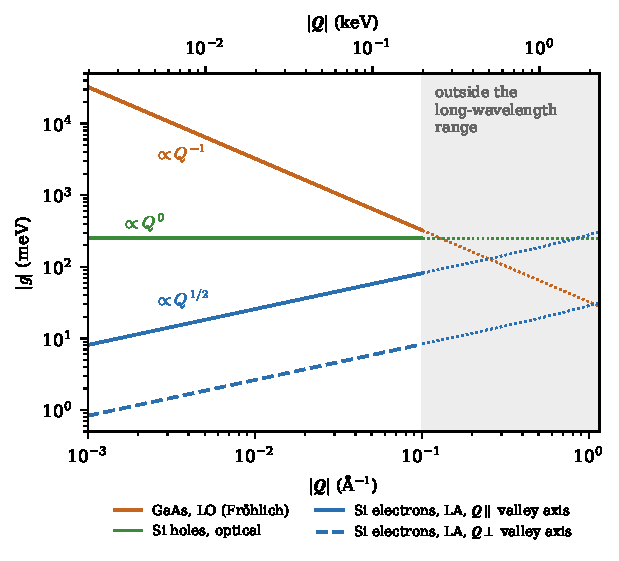
\includegraphics[width=0.72\linewidth]{figures/ch06/fig6_2.pdf}
  \caption{Magnitude of the electron--phonon vertex $|g|$, in the normalization in which $H_{\mathrm{ep}}$ carries $N^{-1/2}$, against the phonon wavevector $|\vect{Q}|$ (bottom axis in \si{\angstrom^{-1}}, top axis in keV), for the three long-wavelength forms of this section. Orange: Fr\"ohlich vertex \cref{eq:6.2-frohlich} of GaAs for an electron at the conduction-band minimum, with $\rho_{nn} = 1$ and the measured $\omega_{\mathrm{L}} = \SI{36.35}{meV}$, $\varepsilon_\infty = 10.88$, $\varepsilon_0 = 12.9$. Green: optical deformation potential \cref{eq:6.2-d} for the holes at the valence maximum of silicon, with the DFPT value \SI{10.45}{eV.\angstrom^{-1}} combined over the degenerate bands~\cite{li2021deformation} and $\omega = \SI{64.1}{meV}$. Blue: acoustic deformation potential \cref{eq:6.2-D} for an electron in a conduction valley of silicon and the longitudinal acoustic phonon, with $\vect{Q}$ along the valley axis (solid, $\Xi_d + \Xi_u = \SI{9.85}{eV}$) and perpendicular to it (dashed, $\Xi_d = \SI{1.01}{eV}$). These use the DFPT constants of Ref.~\cite{li2021deformation} and the DFPT longitudinal acoustic branch along $\mathrm{\Gamma}$--X of \cref{fig:5-si}, whose small-$Q$ slope is \SI{8.34}{km.s^{-1}} (measured: \SI{8.43}{km.s^{-1}}). The curves are these limiting forms, not vertices computed point by point. They are drawn solid up to \SI{0.1}{\angstrom^{-1}}, the end of the range over which the acoustic vertices of silicon were computed and found linear in $Q$~\cite[Fig.~5]{li2021deformation}. Beyond it they are dotted, in the shaded region up to the zone boundary of silicon at $2\pi/a = \SI{1.157}{\angstrom^{-1}}$. On logarithmic axes the slopes $-1$, 0 and $\tfrac12$ distinguish the polar, optical and acoustic couplings.}
  \label{fig:6-gQ}
\end{figure}

\subsection{Wannier interpolation of the vertex}

A phonon-assisted rate in silicon with an energy resolution of \SI{14}{meV} needs the vertex at about $4\times10^9$ pairs $(\vect{k},\vect{Q})$, for every pair of bands and every branch (\cref{app:E.5}). Density-functional perturbation theory costs about one ground-state calculation per phonon wavevector, and a few hundred wavevectors, a $6^3$ or $8^3$ grid, are what a calculation can afford. The step from such a \emph{coarse grid} to the \emph{fine grids} of a rate is an interpolation, and it works for the same reason as the interpolation of bands in \cref{sec:3.6}: in a suitable real-space representation the vertex is short-ranged.

The representation uses Wannier functions for the electrons and single displaced atoms for the phonons. We insert the Bloch sums of Wannier functions of one gauge, $\psi_{n\vect{k}} = N^{-1/2}\sum_{\vect{R}}\ee^{\ii\vect{k}\cdot\vect{R}}\sum_{n'}w_{n'}(\vect{r} - \vect{R})\,U^\dagger_{n'n}(\vect{k})$ (\cref{eq:A.5-wannier} inverted), into the matrix element of $\partial_{\kappa\alpha,\vect{Q}}V_{\mathrm{KS}} = \sum_{\vect{R}_p}\ee^{\ii\vect{Q}\cdot\vect{R}_p}\,\partial V_{\mathrm{KS}}/\partial u^\alpha_{\vect{R}_p\kappa}$. We then translate every term by the cell of the bra and sum over that cell, which cancels the factor $1/N$. What is left is
\begin{gather}
  \bigl\langle\psi_{m,\vect{k}+\vect{Q}}\bigr|\partial_{\kappa\alpha,\vect{Q}}V_{\mathrm{KS}}\bigl|\psi_{n\vect{k}}\bigr\rangle
  = \sum_{\vect{R}_e\vect{R}_p}\ee^{\ii(\vect{k}\cdot\vect{R}_e + \vect{Q}\cdot\vect{R}_p)}\,
  \bigl[U(\vect{k}+\vect{Q})\,g^W_{\kappa\alpha}(\vect{R}_e,\vect{R}_p)\,U^\dagger(\vect{k})\bigr]_{mn} ,
  \nonumber\\
  g^W_{m'n'\kappa\alpha}(\vect{R}_e,\vect{R}_p) = \Bigl\langle w_{m'}(\vect{r})\Bigr|\frac{\partial V_{\mathrm{KS}}}{\partial u^\alpha_{\vect{R}_p\kappa}}\Bigl|w_{n'}(\vect{r} - \vect{R}_e)\Bigr\rangle .
  \label{eq:6.2-gW}
\end{gather}
The real-space vertex $g^W$ is the matrix element, between a Wannier function at the origin and one in cell $\vect{R}_e$, of the screened potential change when a single atom in cell $\vect{R}_p$ moves. Multiplying by the polarization factors of \cref{eq:A.6-g} gives \cref{eq:E.5-ginterp}, and on the coarse grids the relation is inverted by a discrete Fourier transform, as for $H^W(\vect{R})$ in \cref{eq:3.6-HWR}. This is the scheme of Giustino, Cohen and Louie~\cite{giustino2007electron}, reviewed in Ref.~\cite[Eqs.~(177)--(179)]{giustino2017electron} and implemented in the Electron--Phonon Wannier (EPW) code~\cite{ponce2016epw}.

The real-space vertex decays in both of its lattice vectors. In $\vect{R}_e$ it decays as the overlap of two Wannier functions does, exponentially for the smooth gauges of \cref{sec:3.6}, because both must reach the region where the potential changes. In $\vect{R}_p$ it decays as the screened potential of one displaced atom, seen from the Wannier function at the origin. In a nonpolar insulator this potential has neither a monopole, since the displaced atom is screened to neutrality, nor a dipole, since $Z^* = 0$. It still has a quadrupole, and the vertex falls off as $R_p^{-3}$, a tail of no finite range whose Fourier transform carries a term of order $Q^0$ that depends on the direction of $\vect{Q}$. In silicon this quadrupolar part is small, and it can be subtracted like the dipole of a polar crystal below. By the argument that led to \cref{eq:3.6-exact}, a coarse grid whose supercell contains the short-ranged remainder of $g^W$ reproduces the vertex everywhere, and the tails beyond it set the error. For diamond and silicon a $6^3$ or $8^3$ coarse grid of phonon wavevectors is enough (\cref{app:E.5}).

A polar crystal breaks the argument. The displaced atom carries the dipole $eZ^*_\kappa\cdot\vect{u}$ screened by $\varepsilon_\infty$, its potential falls off as $R_p^{-2}$, and the Fourier transform of that tail is the $1/Q$ singularity of the Fr\"ohlich vertex. No finite sum of Fourier components reproduces a singularity. The remedy is the one that \cref{sec:5.5} used for the nonanalytic part of the dynamical matrix. The long-range vertex is known in closed form from $Z^*_\kappa$ and $\varepsilon_\infty$ alone, \cref{eq:D.14-gL} or its version with the sum over reciprocal-lattice vectors, \cref{eq:E.5-gL}. One subtracts it from the coarse-grid vertices, interpolates the short-range remainder $g^{\mathrm{S}} = g - g^{\mathrm{L}}$, which is as smooth as the vertex of a nonpolar crystal, and adds $g^{\mathrm{L}}$ back analytically at every fine-grid point~\cite{verdi2015frohlich}. The split $g = g^{\mathrm{S}} + g^{\mathrm{L}}$ is not unique, since any smooth function can be moved from one part to the other, but every choice puts the whole singularity into $g^{\mathrm{L}}$, and that is all the interpolation needs. The density vertex in $g^{\mathrm{L}}$ is needed at the fine-grid points too, and at small $\vect{Q}$ it is $[U(\vect{k}+\vect{Q})U^\dagger(\vect{k})]_{mn}$ in the Wannier gauge, so that $g^{\mathrm{S}}$ and $g^{\mathrm{L}}$ carry the same phases (\cref{app:A.5}). The quadrupolar terms, present in silicon as in GaAs and, together with the Born charges, the origin of the piezoelectric vertex of GaAs, are long-ranged in the same way and are subtracted with the dipole where the code allows it (\cref{app:E.5}).

\begin{figure}[tbp]
  \centering
  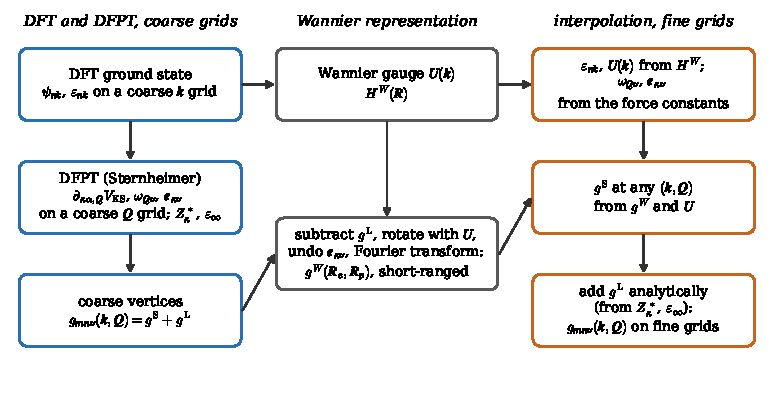
\includegraphics[width=\linewidth]{figures/ch06/fig6_3.pdf}
  \caption{From first principles to interpolated electron--phonon vertices. Left: a density-functional calculation on a coarse grid of crystal momenta gives the Bloch states and energies. Density-functional perturbation theory on a coarse grid of phonon wavevectors gives the screened potential changes $\partial_{\kappa\alpha,\vect{Q}}V_{\mathrm{KS}}$, the phonons, and in a polar crystal $Z^*_\kappa$ and $\varepsilon_\infty$. Their matrix elements are the coarse vertices, \cref{eq:6.2-g}. Middle: the Bloch states define the Wannier gauge $U(\vect{k})$; the long-range part $g^{\mathrm{L}}$ is subtracted, and the rotated remainder is transformed to the real-space vertex $g^W(\vect{R}_e,\vect{R}_p)$ of \cref{eq:6.2-gW}, short-ranged in both lattice vectors. Right: the real-space Hamiltonian and force constants give bands, gauge matrices and phonons at any point; $g^W$ is transformed back, \cref{eq:E.5-ginterp}, and $g^{\mathrm{L}}$, \cref{eq:E.5-gL}, is added analytically. Every quantity in one amplitude uses the same $U(\vect{k})$.}
  \label{fig:6-chain}
\end{figure}

\Cref{fig:6-chain} summarizes the chain. Its pitfalls are practical: a Wannier manifold that misses the states a rate needs, a coarse grid that misplaces the conduction minimum of silicon, a gauge that differs between $g$ and $\rho$. \Cref{app:E.5} discusses each, with the grid sizes, the counts of matrix elements and the checks against direct DFPT at points off the coarse grid. The result is a vertex at any $(\vect{k},\vect{Q})$ for about the cost of a few hundred phonon calculations.

\section{Electron self-energy from phonons}\label{sec:6.3}

At \SI{10}{mK} a silicon crystal holds no thermal phonons, yet its band gap is about \SI{60}{meV} smaller than the gap of the same crystal with its nuclei frozen at their equilibrium positions. The zero-point motion of \cref{sec:5.3}, with a root-mean-square amplitude of \SI{0.05}{\angstrom} along each axis, moves the bands by an amount that matters near threshold: the lightest dark-matter mass a detector can see scales with the gap (\cref{eq:1.3-mmin}). The same coupling decides how long a conduction electron with a few meV of excess energy keeps that energy before it hands it to the lattice. Both effects are the electron self-energy of \cref{sec:4.7}, with phonons as the boson.

\subsection{Fan--Migdal and Allen--Heine terms}

A displaced nucleus changes the potential that the electrons feel, at first and at second order in the displacement. Expanding the self-consistent potential $V_{\mathrm{KS}}$ about equilibrium,
\begin{equation*}
  V_{\mathrm{KS}} = V^{(0)}_{\mathrm{KS}} + \sum_a\frac{\partial V_{\mathrm{KS}}}{\partial u_a}\,u_a + \frac12\sum_{ab}\frac{\partial^2V_{\mathrm{KS}}}{\partial u_a\,\partial u_b}\,u_au_b ,
\end{equation*}
with $a = (\vect{R}\kappa\alpha)$ running over cells, species and Cartesian directions. The linear term is the electron--phonon Hamiltonian $H_{\mathrm{ep}}$ of \cref{eq:6.1-Hep}, with the screened vertex $g_{mn\nu}(\vect{k},\vect{Q})$ of \cref{sec:6.2}. The quadratic term, with each displacement expanded in normal modes by \cref{eq:A.6-u}, is a vertex with two phonon operators,
\begin{equation}
  \begin{gathered}
  H^{(2)}_{\mathrm{ep}} = \frac1N\sum_{\vect{k}\vect{Q}\vect{Q}'}\sum_{mn\nu\nu'}g^{\mathrm{AH}}_{mn\nu\nu'}(\vect{k},\vect{Q},\vect{Q}')\,c^\dagger_{m,\vect{k}+\vect{Q}+\vect{Q}'}c_{n\vect{k}}\,B_{\vect{Q}\nu}B_{\vect{Q}'\nu'} , \\
  g^{\mathrm{AH}}_{mn\nu\nu'}(\vect{k},\vect{Q},\vect{Q}') = \frac{1}{2}\sum_{\kappa\alpha,\kappa'\beta}\frac{e^\alpha_{\kappa\nu}(\vect{Q})\,e^\beta_{\kappa'\nu'}(\vect{Q}')}{\sqrt{2M_\kappa\omega_{\vect{Q}\nu}\,2M_{\kappa'}\omega_{\vect{Q}'\nu'}}}\,\bigl\langle\psi_{m,\vect{k}+\vect{Q}+\vect{Q}'}\big|\partial^2_{\kappa\alpha\vect{Q},\kappa'\beta\vect{Q}'}V_{\mathrm{KS}}\big|\psi_{n\vect{k}}\bigr\rangle ,
  \end{gathered}
  \label{eq:6.3-HAH}
\end{equation}
where $\partial^2_{\kappa\alpha\vect{Q},\kappa'\beta\vect{Q}'}V_{\mathrm{KS}}$ is the second derivative with respect to two displacement waves, the sum over $\vect{R}$ and $\vect{R}'$ of $\ee^{\ii\vect{Q}\cdot\vect{R}+\ii\vect{Q}'\cdot\vect{R}'}$ times the second derivative with respect to $u^\alpha_{\vect{R}\kappa}$ and $u^\beta_{\vect{R}'\kappa'}$ (\cref{app:D.16}). This is the Allen--Heine vertex $g^{\mathrm{AH}}$ (\cref{app:A.6}). In the energy of an electron, $H_{\mathrm{ep}}$ enters at second order and $H^{(2)}_{\mathrm{ep}}$ at first order, and both carry two factors of the zero-point length $\ell_{\vect{Q}\nu}$: they are of the same order, $\langle u^2\rangle$, and a consistent theory keeps both. We will see below that dropping either violates translation invariance.

The first term is the boson-exchange diagram of \cref{sec:4.8} (\cref{fig:4-diagrams}c): the electron emits or absorbs a phonon, propagates in another band and wavevector, and reabsorbs or re-emits it. Compared with \cref{eq:4.8-sigmaboson}, the vertex carries $1/\sqrt N$ instead of $1/\sqrt \Vol$ and band indices, and the intermediate electron can be in any band $m$. The second term needs no propagator at all. Its two phonon operators are contracted with each other, a phonon line that leaves and returns to the same point of the electron line, and the pair is replaced by its thermal average $\langle B_{\vect{Q}\nu}B_{-\vect{Q}\nu}\rangle = 2n_{\vect{Q}\nu} + 1$. \Cref{app:D.16} carries out the Matsubara sum and the continuation for both diagrams.
\begin{keyresult}[Fan--Migdal and Allen--Heine self-energies]
For a nondegenerate band $n$ at wavevector $\vect{k}$, with energies $\omega$ and $\xi_{m\vect{p}} = \varepsilon_{m\vect{p}} - \mu_{\mathrm{ch}}$ measured from the chemical potential, $f_{m\vect{p}} = n_{\mathrm{F}}(\xi_{m\vect{p}})$ and $n_{\vect{Q}\nu} = n_{\mathrm{B}}(\omega_{\vect{Q}\nu})$,
\begin{gather}
  \begin{aligned}
  \Sigma^{\mathrm{FM}}_{n\vect{k}}(\omega) = \frac1N\sum_{\vect{Q}\nu m}|g_{mn\nu}(\vect{k},\vect{Q})|^2
  \biggl[&\frac{n_{\vect{Q}\nu} + 1 - f_{m,\vect{k}+\vect{Q}}}{\omega - \xi_{m,\vect{k}+\vect{Q}} - \omega_{\vect{Q}\nu} + \ii0^+} \\
  &+ \frac{n_{\vect{Q}\nu} + f_{m,\vect{k}+\vect{Q}}}{\omega - \xi_{m,\vect{k}+\vect{Q}} + \omega_{\vect{Q}\nu} + \ii0^+}\biggr] ,
  \end{aligned}
  \label{eq:6.3-FM}\\
  \Sigma^{\mathrm{AH}}_{n\vect{k}} = \frac1N\sum_{\vect{Q}\nu}g^{\mathrm{AH}}_{nn\nu\nu}(\vect{k},\vect{Q},-\vect{Q})\,(2n_{\vect{Q}\nu} + 1) .
  \label{eq:6.3-AH}
\end{gather}
The Fan--Migdal term depends on frequency and has an imaginary part; the Allen--Heine term is static and real.
\end{keyresult}
\Cref{eq:6.3-FM} is the second-order self-energy of Fan~\cite{fan1951temperature}, called the Migdal self-energy in the theory of metals~\cite{migdal1958interaction}, and \cref{eq:6.3-AH} is the term added by Allen and Heine~\cite{allen1976theory}; together they are Ref.~\cite[Eqs.~(157), (158), (160) and~(161)]{giustino2017electron}. The thermal factors read as in \cref{sec:4.8}. In the emission term, $n + 1$ is stimulated plus spontaneous emission and $-f$ blocks an occupied intermediate state. In the absorption term, $n$ counts the phonons present, and $f$ adds the process in which an electron already in $(m,\vect{k}+\vect{Q})$ emits a phonon and drops into the state. The sum over $m$ now runs over occupied bands as well. For a degenerate level, such as the threefold valence maximum of silicon (\cref{sec:3.3}), the self-energy is a matrix in the partners, and the terms between partners, whose denominators vanish, are left out as the term $m = n$ at $\vect{Q} = 0$ is~\cite[Sect.~III\,A]{ponce2015temperature}. Summed over the whole zone, the matrix commutes with the symmetry operations that leave $\vect{k}$ unchanged. On a level whose partners form one irreducible representation it is therefore a multiple of the identity, and every partner shifts by the average of the diagonal elements over the level. This is how the shifts of degenerate band edges below are defined. At $T = 0$ the zero-point motion enters $\Sigma^{\mathrm{FM}}$ through the $1$ of $n + 1$ and through $f$, and $\Sigma^{\mathrm{AH}}$ through the $1$ of $2n + 1$. One more diagram of the same order, a phonon line at zero wavevector ending on a closed electron loop, vanishes because the expansion is made about the minimum of the Born--Oppenheimer surface (\cref{app:D.16}).

The pole of the Dyson equation \cref{eq:4.7-dyson} then sits at the renormalized band energy
\begin{equation}
  \varepsilon^{\mathrm{ren}}_{n\vect{k}} = \varepsilon_{n\vect{k}} + \Real\Sigma^{\mathrm{FM}}_{n\vect{k}}(\varepsilon^{\mathrm{ren}}_{n\vect{k}}) + \Sigma^{\mathrm{AH}}_{n\vect{k}} ,
  \label{eq:6.3-ren}
\end{equation}
with $\omega$ now measured from the same origin as $\varepsilon$, the quasiparticle condition of \cref{eq:4.7-qp}. Its value at $T = 0$, less $\varepsilon_{n\vect{k}}$, is the \emph{zero-point renormalization} (ZPR) of the state, and the ZPR of a gap is that of the conduction state minus that of the valence state. The theory built on the two terms, usually in the adiabatic form below and with the rigid-ion approximation of Allen and Cardona~\cite{allen1981temperature}, is called Allen--Heine--Cardona (AHC) theory. In practice $\Sigma^{\mathrm{FM}}$ is often evaluated at $\omega = \varepsilon_{n\vect{k}}$ rather than at the solution of \cref{eq:6.3-ren}; for the Einstein boson of \cref{we:4-einstein} the two choices yield \SI{-9.14}{meV} and \SI{-8.73}{meV}, a difference set by $1 - z_{\mathrm{qp}}$.

\subsection{The adiabatic limit}

Where the phonon energies are small next to the electronic energy differences that dominate the sum over $m$, they can be dropped from the denominators of \cref{eq:6.3-FM}. Setting also $\omega = \varepsilon_{n\vect{k}}$, the two terms acquire the same denominator, and their numerators add to $(n + 1 - f) + (n + f) = 2n + 1$: the occupations of the intermediate states drop out. The result is the formula of Allen and Heine~\cite{allen1976theory},
\begin{equation}
  \varepsilon^{\mathrm{ren}}_{n\vect{k}} - \varepsilon_{n\vect{k}} = \frac1N\sum_{\vect{Q}\nu}(2n_{\vect{Q}\nu} + 1)\Biggl[\sum_m\frac{|g_{mn\nu}(\vect{k},\vect{Q})|^2}{\varepsilon_{n\vect{k}} - \varepsilon_{m,\vect{k}+\vect{Q}}} + g^{\mathrm{AH}}_{nn\nu\nu}(\vect{k},\vect{Q},-\vect{Q})\Biggr] ,
  \label{eq:6.3-adiabatic}
\end{equation}
Ref.~\cite[Eq.~(167)]{giustino2017electron}. Every mode now enters with the weight $2n_{\vect{Q}\nu} + 1$ of its mean-square displacement (\cref{eq:5.3-B}). Allen and Heine derived \cref{eq:6.3-adiabatic} without diagrams. With the nuclei frozen at displacements $u_a$, a band energy is a function $\varepsilon_{n\vect{k}}(\{u\})$, and second-order perturbation theory gives its curvature: the Fan sum is the second-order term of $H_{\mathrm{ep}}$, the Allen--Heine vertex the first-order term of the quadratic potential (\cref{eq:D.16-frozen}). The nuclei are not frozen, however, but spread over a Gaussian distribution of width $\langle u_au_b\rangle$. Averaged over it, the linear term vanishes and the energy shifts by half the curvature times the width, $\tfrac12\sum_{ab}\langle u_au_b\rangle\,\partial^2\varepsilon_{n\vect{k}}/\partial u_a\partial u_b$. In the adiabatic limit the AHC shift is the average of the band energy over the zero-point and thermal smearing of the lattice.

The adiabatic form fails where the dropped phonon energies are not small. That happens for $m = n$ at small $Q$, where $\varepsilon_{n\vect{k}} - \varepsilon_{n,\vect{k}+\vect{Q}}$ vanishes with $Q$, and wherever another band is degenerate with the state. Both occur at band edges, the states that set a detector's threshold. The Fr\"ohlich vertex of a polar crystal shows how badly it can fail. Take an electron at the bottom of a parabolic band of mass $m^*$ at $T = 0$, coupled to the longitudinal optical phonon by $|g^{\mathrm{L}}|^2 = C_{\mathrm{F}}^2/Q^2$ (\cref{eq:6.2-frohlich}). In the adiabatic form its intraband Fan term is
\begin{equation*}
  \frac1N\sum_{\vect{Q}}\frac{|g^{\mathrm{L}}|^2}{-Q^2/2m^*} = -\Omega\int\frac{\dd^3Q}{(2\pi)^3}\,\frac{2m^*C_{\mathrm{F}}^2}{Q^4} = -\frac{\Omega\,m^*C_{\mathrm{F}}^2}{\pi^2}\int_0\frac{\dd Q}{Q^2} ,
\end{equation*}
which diverges at small $Q$. The divergence is an artifact. With the phonon energy kept, only the emission term of \cref{eq:6.3-FM} survives for an empty band at $T = 0$, its denominator at $\omega = \varepsilon_{n\vect{k}}$ is $-Q^2/2m^* - \omega_{\mathrm{L}}$, and $\Real\Sigma^{\mathrm{FM}}$ is the finite second-order shift of \cref{sec:6.2}, $-\alpha_{\mathrm{F}}\omega_{\mathrm{L}} = -\SI{2.6}{meV}$ for the conduction band of GaAs (\cref{we:6-frohlich}). The Fr\"ohlich polaron shift is the Fan--Migdal self-energy at the band bottom. Every infrared-active crystal has this $1/Q^2$ coupling. For all of them the adiabatic ZPR is infinite, and the nonadiabatic form, with the phonon energies in the denominators, is needed to get a number~\cite{ponce2015temperature}. In silicon the vertex has no $1/Q$ term (\cref{sec:6.2}), both forms converge, and they differ by \SI{8}{meV}: \SI{-64.3}{meV} adiabatic and \SI{-56.2}{meV} nonadiabatic for the indirect gap in the local-density approximation~\cite[Table~VI]{ponce2015temperature}.

\subsection{Translation invariance and the rigid-ion approximation}

Moving the whole crystal by a constant vector shifts no band energy. For long-wavelength acoustic phonons this ties the Fan and Allen--Heine terms together. As $Q \to 0$ an acoustic mode becomes a rigid translation, with $\vect{e}_{\kappa\nu} \to (M_\kappa/M_{\mathrm{cell}})^{1/2}\hat{\vect{e}}_\nu$ and every nucleus displaced by $\ell_{\vect{Q}\nu}\hat{\vect{e}}_\nu/\sqrt N$ per unit of $B_{\vect{Q}\nu}$ (\cref{app:A.6}). Its vertex then follows from \cref{eq:6.2-g} and the acoustic sum rule \cref{eq:6.2-asr},
\begin{equation*}
  g_{mn\nu}(\vect{k},\vect{Q}) \to \ell_{\vect{Q}\nu}\sum_\kappa\hat{\vect{e}}_\nu\cdot\bigl\langle\psi_{m\vect{k}}\bigr|\partial_{\kappa,\vect{0}}V_{\mathrm{KS}}\bigl|\psi_{n\vect{k}}\bigr\rangle = -\ii\,\ell_{\vect{Q}\nu}\,(\varepsilon_{n\vect{k}} - \varepsilon_{m\vect{k}})\,\hat{\vect{e}}_\nu\cdot\vect{p}_{mn}(\vect{k}) .
\end{equation*}
The intraband element vanishes, as \cref{sec:6.2} showed; the interband elements do not. In the Fan sum of \cref{eq:6.3-adiabatic} the energy difference is squared in the numerator and appears once in the denominator. What is left is
\begin{equation*}
  \sum_{m\ne n}\frac{|g_{mn\nu}|^2}{\varepsilon_{n\vect{k}} - \varepsilon_{m\vect{k}}} \to \ell_{\vect{Q}\nu}^2\sum_m(\varepsilon_{n\vect{k}} - \varepsilon_{m\vect{k}})\,|\hat{\vect{e}}_\nu\cdot\vect{p}_{mn}|^2 .
\end{equation*}
For the Allen--Heine vertex of the same mode, the same polarization vectors turn the prefactor of \cref{eq:6.3-HAH} into $\ell_{\vect{Q}\nu}^2\hat e_{\nu\alpha}\hat e_{\nu\beta}$, and the second derivative with respect to two displacement waves of zero wavevector, summed over $\kappa$ and $\kappa'$, becomes the second derivative with respect to a uniform translation $\vect{t}$ of the whole crystal. The self-consistent potential moves with the crystal, $V_{\mathrm{KS}} \to \op{T}_{\vect{t}}V_{\mathrm{KS}}\op{T}^\dagger_{\vect{t}}$ with $\op{T}_{\vect{t}} = \ee^{-\ii\vect{t}\cdot\op{\vect{p}}}$ (\cref{sec:6.2}). Differentiating twice along $\hat{\vect{e}}_\nu$ gives $-[\op{p}_\nu,[\op{p}_\nu,V_{\mathrm{KS}}]]$ with $\op{p}_\nu = \hat{\vect{e}}_\nu\cdot\op{\vect{p}}$, and since the kinetic energy commutes with $\op{p}_\nu$, $V_{\mathrm{KS}}$ may be replaced by $H_{\mathrm{KS}}$. Expanding the double commutator in the eigenstates of $H_{\mathrm{KS}}$ at $\vect{k}$, the states that $\op{p}_\nu$ connects to $\psi_{n\vect{k}}$,
\begin{equation*}
  g^{\mathrm{AH}}_{nn\nu\nu}(\vect{k},\vect{Q},-\vect{Q}) \to -\frac{\ell_{\vect{Q}\nu}^2}{2}\bigl\langle\psi_{n\vect{k}}\bigr|[\op{p}_\nu,[\op{p}_\nu,H_{\mathrm{KS}}]]\bigl|\psi_{n\vect{k}}\bigr\rangle = -\ell_{\vect{Q}\nu}^2\sum_m(\varepsilon_{n\vect{k}} - \varepsilon_{m\vect{k}})\,|\hat{\vect{e}}_\nu\cdot\vect{p}_{mn}|^2 .
\end{equation*}
The two contributions cancel term by term:
\begin{equation}
  \sum_{m\ne n}\frac{|g_{mn\nu}(\vect{k},\vect{Q})|^2}{\varepsilon_{n\vect{k}} - \varepsilon_{m,\vect{k}+\vect{Q}}} + g^{\mathrm{AH}}_{nn\nu\nu}(\vect{k},\vect{Q},-\vect{Q}) \to 0 \qquad (\nu \text{ acoustic},\ Q \to 0) .
  \label{eq:6.3-cancel}
\end{equation}
The picture is the one of \cref{sec:6.2}. The interband vertex translates the electronic state along with the crystal, and at second order it shifts the energy by $\ell_{\vect{Q}\nu}^2\sum_m(\varepsilon_{n\vect{k}} - \varepsilon_{m\vect{k}})|\hat{\vect{e}}_\nu\cdot\vect{p}_{mn}|^2$, a sum of either sign: bands above $n$ push it down, bands below push it up. The Allen--Heine term measures the curvature of the potential under the same translation, and it shifts the energy back by exactly as much. Neither term means anything alone, and a calculation must treat both on the same grid of wavevectors. In the language of scalar quantum electrodynamics (QED) the two are the rainbow and the seagull diagrams, and their cancellation for a rigid translation is the analogue of the one that makes the scattering of low-frequency light by a bound electron vanish. The same double commutator underlies the f-sum rule (\cref{eq:4.3-firstmoment}). The three translational modes at exactly $\vect{Q} = 0$, with zero frequency, are left out of both sums; \cref{eq:6.3-cancel} states that the integrand is continuous there. For small $Q$ the first correction to the cancellation is linear in $\vect{Q}$ and drops out of the sum over directions. The interband remainder is then smaller by a factor $\sim Q^2$, and long-wavelength acoustic phonons, which carry a large share of the thermal $\langle u^2\rangle$ of silicon (\cref{we:5-u2}), barely shift the bands. What survives at small $Q$ is the intraband term, $m = n$, whose denominator vanishes with $Q$, the term that needs the phonon energy kept.

The Allen--Heine vertex needs second derivatives of the self-consistent potential, a second-order perturbation calculation that few codes perform. Translation invariance offers a way around it. A rigid translation leaves every band energy unchanged at every configuration of the nuclei, so the sum over all nuclei of $\partial\varepsilon_{n\vect{k}}/\partial u_{\vect{R}\kappa\alpha}$ vanishes everywhere, and so does its derivative. At equilibrium this is an exact sum rule, \cref{eq:D.16-sr2}: the diagonal element of the second derivative, summed over the sites of the whole crystal, equals a product of first derivatives at $\vect{Q} = 0$. The sum rule fixes a sum over sites, while $g^{\mathrm{AH}}$ needs the on-site element. The \emph{rigid-ion approximation} supplies the missing step. It writes the potential as a sum of atom-centered terms that move rigidly with their nuclei, $V_{\mathrm{KS}} = \sum_{\vect{R}\kappa}v_\kappa(\vect{r} - \vect{R} - \vect{\tau}_\kappa - \vect{u}_{\vect{R}\kappa})$. Second derivatives with respect to two different atoms then vanish, the sum rule determines the on-site element (\cref{eq:D.16-ria}), and the Allen--Heine term becomes
\begin{equation}
  \Sigma^{\mathrm{AH}}_{n\vect{k}} = -\frac12\sum_{\kappa\kappa'}\sum_{\alpha\beta}\bigl(B^{\alpha\beta}_\kappa + B^{\alpha\beta}_{\kappa'}\bigr)\,\Real{\sum_{m}}'\frac{\langle\psi_{n\vect{k}}|\partial_{\kappa\alpha,\vect{0}}V_{\mathrm{KS}}|\psi_{m\vect{k}}\rangle\,\langle\psi_{m\vect{k}}|\partial_{\kappa'\beta,\vect{0}}V_{\mathrm{KS}}|\psi_{n\vect{k}}\rangle}{\varepsilon_{n\vect{k}} - \varepsilon_{m\vect{k}}} ,
  \label{eq:6.3-ria}
\end{equation}
where $B_\kappa = \langle\vect{u}_\kappa\vect{u}_\kappa\rangle$ is the displacement tensor of \cref{eq:5.3-B} at temperature $T$ and the prime excludes the states degenerate with $(n,\vect{k})$ (\cref{app:D.16}). This is the form of Allen and Cardona~\cite{allen1981temperature}, Ref.~\cite[Eqs.~(195)--(198)]{giustino2017electron}. It needs just the first-order potentials at $\vect{Q} = 0$, which every phonon calculation already supplies. Its structure is a Fan term at zero wavevector with the opposite sign, weighted by the mean-square displacement of each atom; the cancellation of \cref{eq:6.3-cancel} is built in. What it neglects is the change of screening when two atoms move together rather than one at a time. Poncé et al.\ find that correction large in molecules~\cite{ponce2015temperature}; for crystals the rigid-ion form is the standard choice.

In practice the AHC shift is computed from DFPT vertices on a grid of phonon wavevectors. The sum over bands is split into an active window, summed explicitly, and the rest, obtained from a Sternheimer equation. The sum over $\vect{Q}$ converges slowly near the vanishing intraband denominators and needs grids of $10^5$ to $10^6$ points, or Wannier interpolation of the vertex (\cref{sec:6.2}), with a small imaginary part in the denominators extrapolated to zero. \Cref{app:E.8} describes the calculation, its convergence parameters and its pitfalls, among them the small residual Born charges of a nonpolar DFPT calculation, which must be removed before the sum or the integral diverges at a band extremum.

\subsection{Smeared ionic potentials}

The literature calls $\Sigma^{\mathrm{AH}}$ the Debye--Waller self-energy, and in the rigid-ion approximation the name has a reason. Average the rigid-ion potential over the Gaussian distribution of the displacements of each nucleus. A Fourier component $v_\kappa(\vect{G})\,\ee^{\ii\vect{G}\cdot(\vect{r} - \vect{R} - \vect{\tau}_\kappa)}$ acquires the factor $\langle\ee^{-\ii\vect{G}\cdot\vect{u}_\kappa}\rangle = \ee^{-\vect{G}\cdot B_\kappa\cdot\vect{G}/2}$, and to first order in $B_\kappa$
\begin{equation}
  \bigl\langle v_\kappa(\vect{r} - \vect{u}_\kappa)\bigr\rangle - v_\kappa(\vect{r}) = \frac12\sum_{\alpha\beta}B^{\alpha\beta}_\kappa\,\partial_\alpha\partial_\beta v_\kappa(\vect{r}) = -\sum_{\vect{G}}W_\kappa(\vect{G})\,v_\kappa(\vect{G})\,\ee^{\ii\vect{G}\cdot\vect{r}} ,
  \label{eq:6.3-smear}
\end{equation}
for the atom at the origin, with $2W_\kappa(\vect{G}) = \vect{G}\cdot B_\kappa\cdot\vect{G}$, the exponent of \cref{eq:5.6-W} evaluated at a reciprocal-lattice vector. The diagonal matrix element of the middle expression, summed over all the sites of every species, is the rigid-ion Allen--Heine term (\cref{app:D.16}). So $\Sigma^{\mathrm{AH}}$ is the first-order change of a band energy when each ionic potential is smeared out by the zero-point and thermal motion of its nucleus, the ``fuzziness'' of the nuclear charge described in Ref.~\cite[below Eq.~(154)]{giustino2017electron}.

It is nonetheless a different object from the Debye--Waller factor $\ee^{-2W_\kappa(\vect{q})}$ of \cref{sec:5.6}, a probability that multiplies a rate at the momentum transfer of the scattering. The smearing of \cref{eq:6.3-smear} involves no momentum transfer and no rate. It is evaluated at the reciprocal-lattice vectors of the static potential, enters an energy at first order in $B_\kappa$, and is one of the two terms of the second-order shift. The Fan term is of the same order and partly cancels it, exactly so for acoustic phonons at small $Q$ (\cref{eq:6.3-cancel}). Allen and Heine showed that a theory of the band shifts with the smeared potential alone is incomplete~\cite{allen1976theory}. The two share the displacement tensor $B_\kappa$, and nothing else.

\subsection{Zero-point renormalization}

For the indirect gap of silicon, AHC theory in the local-density approximation gives a zero-point renormalization of \SI{-56.2}{meV} in the nonadiabatic form~\cite[Table~VI]{ponce2015temperature}. The valence maximum rises and the conduction minimum drops, by \SI{35}{meV} and \SI{22}{meV} in a calculation by a different method~\cite[Sect.~VII\,B]{zacharias2020theory}, and the gap closes from both sides. That calculation used \emph{special displacements}, a non-perturbative route that avoids vertices and sums over wavevectors altogether. Since the adiabatic shift is the average of the band energy over the Gaussian distribution of the nuclei, it can be computed directly: displace the nuclei of a large supercell and compute the bands. Zacharias and Giustino showed that a single configuration suffices, one in which every normal coordinate has its root-mean-square amplitude and the signs alternate between modes so that the cross terms cancel~\cite{zacharias2016one}. In an $8\times8\times8$ supercell of 1024 atoms it yields \SI{-57}{meV}~\cite[Sect.~VII\,B]{zacharias2020theory}. The method includes all orders in the displacements but is adiabatic by construction.

The renormalization extracted from experiment is \SI{-62}{meV} or \SI{-64}{meV}, depending on the route~\cite{cardona2005electron}, as tabulated in Ref.~\cite[Table~VI]{ponce2015temperature}. A ZPR cannot be measured directly, since no experiment freezes the nuclei. Both routes rest on how the shift depends on temperature and on the nuclear mass, which the simplest model makes explicit.

Suppose every phonon has the same energy $\omega_{\mathrm{Ein}}$, an Einstein crystal. The weight $2n_{\vect{Q}\nu} + 1 = \coth(\omega_{\mathrm{Ein}}/2T)$ is then the same for every mode and comes out of the sum in \cref{eq:6.3-adiabatic}. The shift of any band at temperature $T$ is its zero-point value times one function of temperature,
\begin{equation}
  \Delta\varepsilon_{n\vect{k}}(T) = \Delta\varepsilon_{n\vect{k}}(0)\,\coth\frac{\omega_{\mathrm{Ein}}}{2T} .
  \label{eq:6.3-einstein}
\end{equation}
At $T \gg \omega_{\mathrm{Ein}}$, $\coth x \simeq 1/x + x/3$, and the shift becomes linear in $T$ with the slope $2\Delta\varepsilon(0)/\omega_{\mathrm{Ein}}$. Since this line extrapolates to zero shift at $T = 0$, extrapolating a measured gap back from high temperature lands on the gap of the clamped lattice, and the low-temperature gap sits below that intercept by the ZPR. This is one of the two extractions. The other uses the nuclear mass. At fixed force constants $\omega_{\mathrm{Ein}} \propto M^{-1/2}$, the squared vertex and the Allen--Heine term are both proportional to $\ell^2 \propto 1/(M\omega_{\mathrm{Ein}}) \propto M^{-1/2}$, and so is the ZPR. Then $\mathrm{ZPR} = -2M\,\partial\Eg/\partial M$, and the gaps of isotopically enriched crystals measure it.

\begin{workedexample}{The Einstein model of the silicon gap}\label{we:6-zpr}
The Einstein boson of \cref{we:4-einstein} shifted the band bottom by \SI{-9.14}{meV} at $T = 0$ and by \SI{-11.09}{meV} at \SI{300}{K}, a ratio of 1.213 against $2n_{\mathrm{B}} + 1 = 1.218$. The small difference came from the boson energy in the denominators. In the adiabatic limit \cref{eq:6.3-einstein} makes the ratio exact, and the model reduces to two numbers: the ZPR and $\omega_{\mathrm{Ein}}$.

For silicon we choose $\omega_{\mathrm{Ein}}$ by the zero-point motion. At $T = 0$ every term of the ZPR carries a factor $1/\omega_{\vect{Q}\nu}$ from $\ell_{\vect{Q}\nu}^2$, as the mean-square displacement does, and the Einstein energy that reproduces the zero-point $\langle u^2\rangle$ of the computed phonon spectrum is $\langle\omega^{-1}\rangle^{-1} = \SI{30.4}{meV}$, or \SI{353}{K} (\cref{we:5-u2}). For the ZPR we take the nonadiabatic AHC value, \SI{-56.2}{meV}. Applying the adiabatic weight of \cref{eq:6.3-einstein} to a nonadiabatic value is an approximation; the two forms differ by \SI{8}{meV} at $T = 0$.

At \SI{300}{K}, $T = \SI{25.85}{meV}$, $\omega_{\mathrm{Ein}}/2T = 0.588$ and $\coth(0.588) = 1.891$. The model predicts that the gap closes between zero and room temperature by
\begin{equation*}
  \Eg(\SI{300}{K}) - \Eg(0) = -\SI{56.2}{meV}\times(1.891 - 1) = -\SI{50.1}{meV} .
\end{equation*}
The measured gap, $\Eg(T) = \Eg(0) - aT^2/(T + b)$ with $\Eg(0) = \SI{1.1692}{eV}$, $a = \SI{4.9e-4}{eV.K^{-1}}$ and $b = \SI{655}{K}$, a fit to photoluminescence up to \SI{1000}{K}~\cites{alex1996temperature}[Eq.~(11)]{ramanathan2020ionization}, falls by \SI{46.2}{meV}, from \SI{1.1692}{eV} to \SI{1.1230}{eV}. The model is \SI{8}{\percent} high; with the adiabatic ZPR, \SI{-64.3}{meV}, it would predict \SI{-57.3}{meV}. Its high-temperature slope is $2\times\SI{56.2}{meV}/\SI{353}{K} = \SI{0.318}{meV.K^{-1}}$, between the slopes of the measured curve at \SI{300}{K} and \SI{500}{K}, 0.26 and \SI{0.33}{meV.K^{-1}}.

The choice of $\omega_{\mathrm{Ein}}$ carries physics. Had we assumed that the gap follows the full mean-square displacement of the computed spectrum, the shift would have scaled with $\langle u^2\rangle(T)/\langle u^2\rangle(0) = 2.661$, and the gap would have closed by $\SI{56.2}{meV}\times1.661 = \SI{93.3}{meV}$ at \SI{300}{K}, twice the measured value. That assumption gives every mode a shift in proportion to its mean-square displacement, and the thermal $\langle u^2\rangle$ is weighted toward the softest modes, which enter with $1/\omega^2$: the long-wavelength acoustic phonons and the flat transverse acoustic branches near the zone boundary (\cref{we:5-u2}). The measured curve says that these modes move the gap less than their share of $\langle u^2\rangle$, and for the acoustic modes at small $Q$ \cref{eq:6.3-cancel} explains why: they are nearly rigid translations. The gap responds to the displacements of atoms relative to their neighbors, not to their displacement as such.

Two further numbers follow. The model's clamped-lattice gap, the intercept of its high-temperature line, is $\SI{1.1692}{eV} + \SI{0.0562}{eV} = \SI{1.2254}{eV}$; the model is anchored at the measured $\Eg(0)$, which contains the zero-point expansion of the lattice, and it leaves out thermal expansion. And replacing natural silicon, $M = \SI{28.09}{u}$, by $^{30}$Si scales the ZPR by $(28.09/29.97)^{1/2}$ and raises the gap by \SI{1.8}{meV}. At detector temperatures nothing of the thermal part survives. At \SI{1}{K}, $\omega_{\mathrm{Ein}}/T = 353$ and $2n_{\mathrm{B}}(\omega_{\mathrm{Ein}}) \sim 10^{-153}$; the only phonons still occupied are acoustic modes at small $Q$, and their contribution vanishes by \cref{eq:6.3-cancel} and with their phase space. A detector at \SI{10}{mK} therefore sees $\Eg(0)$.
\end{workedexample}

\begin{figure}[tbp]
  \centering
  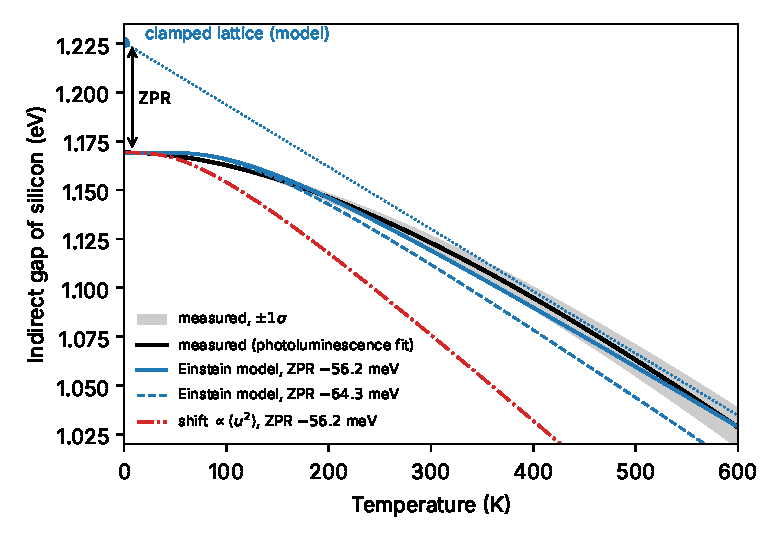
\includegraphics[width=0.8\linewidth]{figures/ch06/fig6_4.pdf}
  \caption{The indirect gap of silicon against temperature. Black: measured, the fit $\Eg(T) = \SI{1.1692}{eV} - aT^2/(T + b)$ with $a = \SI{4.9e-4}{eV.K^{-1}}$ and $b = \SI{655}{K}$ to photoluminescence data~\cite{alex1996temperature,ramanathan2020ionization}; the gray band is the envelope of the fits with $a$ and $b$ varied independently by their quoted errors of \SI{0.2e-4}{eV.K^{-1}} and \SI{40}{K}. Blue: Einstein model $\Eg(0) + \mathrm{ZPR}\,[\coth(\omega_{\mathrm{Ein}}/2T) - 1]$ with $\omega_{\mathrm{Ein}} = \SI{30.4}{meV}$, the Einstein energy that reproduces the zero-point mean-square displacement of the computed phonon spectrum, and the computed zero-point renormalization, \SI{-56.2}{meV} (solid, nonadiabatic) or \SI{-64.3}{meV} (dashed, adiabatic)~\cite{ponce2015temperature}. Red, dash-dotted: a shift proportional to the full mean-square displacement $\langle u^2\rangle(T)$ of the computed spectrum, with the same zero-point value. Blue dotted line and dot: the high-temperature asymptote of the solid model, which extrapolates to the model's clamped-lattice gap, \SI{1.2254}{eV}, at $T = 0$; the arrow marks the ZPR. All model curves are anchored at the measured gap at $T = 0$ and leave out thermal expansion.}
  \label{fig:6-gapT}
\end{figure}

In \cref{fig:6-gapT} the Einstein model with a computed ZPR and an Einstein energy fixed by the zero-point motion follows the measured gap to within about \SI{5}{meV} from zero to \SI{600}{K}. Below \SI{150}{K} it falls slightly too slowly, since a single energy of \SI{30}{meV} cannot represent the softer modes that the real spectrum starts to populate first. The curve that follows $\langle u^2\rangle$ fails from the start.

The values \SI{-62}{meV} and \SI{-64}{meV} extracted from experiment come from the isotope dependence of the gap and from the linear extrapolation of its high-temperature part~\cite{cardona2005electron}, and they need no Einstein energy. They contain the whole zero-point shift of the gap, including a part that is not electron--phonon coupling at all: the zero-point motion also expands the lattice, which by itself opens the gap by \SI{9}{meV}~\cite[Table~S2]{miglio2020predominance}. The electron--phonon part implied by experiment is therefore $-71$ to \SI{-73}{meV}. That is the number to compare with the computed \SI{-56.2}{meV}, a fixed-volume electron--phonon value, and the calculation falls about \SI{20}{\percent} short of it, as does the special-displacement value of \SI{-57}{meV}. The shortfall is consistent with the overscreening of the vertex by the small Kohn--Sham gap: a calculation of the same kind on $GW$ bands gives \SI{66}{meV}~\cite[Sect.~VII\,B]{zacharias2020theory}.

\subsection{Phonon-limited lifetimes}

The imaginary part of the self-energy is a decay rate. The Allen--Heine term is real and contributes nothing to it. For the Fan--Migdal term, the Sokhotski--Plemelj formula \cref{eq:2.4-SP} turns each denominator of \cref{eq:6.3-FM} into a delta function,
\begin{equation}
  \begin{aligned}
  \Imag\Sigma^{\mathrm{FM}}_{n\vect{k}}(\omega) = -\frac{\pi}{N}\sum_{\vect{Q}\nu m}|g_{mn\nu}(\vect{k},\vect{Q})|^2
  \Bigl[&(n_{\vect{Q}\nu} + 1 - f_{m,\vect{k}+\vect{Q}})\,\delta(\omega - \xi_{m,\vect{k}+\vect{Q}} - \omega_{\vect{Q}\nu}) \\
  &+ (n_{\vect{Q}\nu} + f_{m,\vect{k}+\vect{Q}})\,\delta(\omega - \xi_{m,\vect{k}+\vect{Q}} + \omega_{\vect{Q}\nu})\Bigr] ,
  \end{aligned}
  \label{eq:6.3-ImFM}
\end{equation}
and by \cref{eq:4.7-qp} the state decays at the rate $\varGamma_{n\vect{k}} = -2z_{\mathrm{qp}}\Imag\Sigma^{\mathrm{FM}}_{n\vect{k}}(\xi_{n\vect{k}})$, its \emph{phonon-limited lifetime} being $1/\varGamma_{n\vect{k}}$. The cutting rule of \cref{sec:4.8} reads \cref{eq:6.3-ImFM} as golden-rule rates: the cut runs through the intermediate electron and the phonon, and puts both on shell. For an electron in an empty band the out-scattering rates are all that remain, emission of a phonon with the weight $n + 1$ and absorption with the weight $n$ of \cref{eq:A.6-weights}.

At $T = 0$ only emission is left, and an electron can emit only if a state of lower energy is available. An electron at the bottom of the conduction band of an insulator has none, and its width is zero: band edges are sharp at zero temperature, as \cref{sec:4.7} anticipated. A width found at a band extremum at $T = 0$ in a calculation is the imaginary part added to the denominators for numerical reasons, not a lifetime. At \SI{10}{mK} the absorption term is absent for every phonon above about \SI{10}{\micro eV}, and a hot carrier in a detector loses its energy by spontaneous emission only. How fast, and down to what energy?

For a conduction electron near a band minimum the answer is set by acoustic phonons. Take a parabolic band of mass $m^*$, an electron of wavevector $\vect{k}$ measured from the minimum, and the deformation-potential vertex $|g|^2 = \Xi^2Q/(2M_{\mathrm{cell}}c)$ of \cref{eq:6.2-D}, for a branch of sound speed $c$ and an effective constant $\Xi$. At $T = 0$, with $(1/N)\sum_{\vect{Q}} \to \Omega\int\dd^3Q/(2\pi)^3$,
\begin{equation*}
  \varGamma(\vect{k}) = 2\pi\,\Omega\int\frac{\dd^3Q}{(2\pi)^3}\,\frac{\Xi^2Q}{2M_{\mathrm{cell}}c}\;\delta\Bigl(\frac{k^2 - |\vect{k} + \vect{Q}|^2}{2m^*} - cQ\Bigr) .
\end{equation*}
The delta function fixes the angle $\theta$ between $\vect{Q}$ and $\vect{k}$ at $\cos\theta = -(Q/2 + m^*c)/k$, and the integral over $\cos\theta$ gives $m^*/(kQ)$. A solution exists only for $Q \le Q_{\max} = 2(k - m^*c)$, which requires $k > m^*c$: the electron must move faster than sound. The emission is Cherenkov radiation of sound, and the phonons go out on a cone about the direction of motion. The remaining integral over $Q$ gives
\begin{equation}
  \varGamma(\vect{k}) = \frac{\Omega\,\Xi^2\,m^*\,Q_{\max}^3}{12\pi M_{\mathrm{cell}}\,c\,k} , \qquad Q_{\max} = 2(k - m^*c) ,
  \label{eq:6.3-cherenkov}
\end{equation}
which grows linearly with the kinetic energy $k^2/2m^*$ far above the threshold.

For silicon we estimate the rate with three simplifications. The valley is taken spherical, with the density-of-states mass $m^* = m^*_{\mathrm{d}} = (m^*_\parallel m^{*2}_\perp)^{1/3} = 0.322\,m_e$ from the valley masses of \cref{sec:3.3}. The valley constants of \cref{sec:6.2}, $\Xi_d = \SI{1.01}{eV}$ and $\Xi_u = \SI{8.84}{eV}$, enter with their angular factors averaged over the angle between $\vect{Q}$ and the valley axis, as for valleys of random orientation: $\Xi^2 = \Xi_d^2 + \tfrac23\Xi_d\Xi_u + \tfrac15\Xi_u^2 = (\SI{4.75}{eV})^2$ for the longitudinal branch and $\tfrac{2}{15}\Xi_u^2 = (\SI{3.23}{eV})^2$ for the one transverse branch that couples. And the sound speeds are the measured ones along $[100]$, 8.43 and \SI{5.84}{km.s^{-1}} (\cref{sec:5.2}). The thresholds $m^*c^2/2$ are \SI{0.065}{meV} for longitudinal and \SI{0.031}{meV} for transverse emission. At \SI{10}{meV} of kinetic energy the two branches give $\varGamma = 7.2 + \SI{5.2}{\micro eV} = \SI{12.3}{\micro eV}$, a lifetime of \SI{53}{ps}; at \SI{1}{meV} the lifetime is \SI{0.9}{ns}, and at \SI{30}{meV} \SI{16}{ps}. Above the optical phonon energy, \SI{64}{meV}, and through intervalley scattering (\cref{sec:6.2}) the rates are far higher. The estimate fixes the scale. An electron created with a few meV in a silicon detector sheds it as acoustic phonons over a fraction of a nanosecond, and then stops emitting once its kinetic energy falls below a few tens of \si{\micro eV}, under \SI{1}{K}. In a biased detector the field keeps the carriers above that threshold, and the phonons emitted along the drift are the Luke phonons of \cref{sec:20.1}. A quantitative rate uses \cref{eq:6.3-ImFM} with DFPT vertices on fine grids and the real anisotropic valleys.

\subsection{Migdal's adiabatic theorem}

The Fan--Migdal self-energy keeps the vertex $g$ bare at both ends and the propagators free. The exact self-energy has the same structure with every piece dressed: the full electron propagator, the full phonon propagator, and a vertex function in place of one of the two $g$'s~\cite[Eq.~(156)]{giustino2017electron}. At fourth order in $g$ two new diagrams appear. In one, a second phonon line is emitted and reabsorbed inside the first, on the intermediate electron line; it is a self-energy insertion, and replacing the free propagator in \cref{eq:6.3-FM} by the full one sums all such insertions. In the other, the two phonon lines cross. This is a vertex correction, and no self-consistency of the propagators includes it. Migdal's question was how large it is~\cite{migdal1958interaction}.

In a metal, the counting of \cref{sec:6.1} answers it. Consider an electron at the Fermi surface. In the self-energy insertion the inner phonon carries a frequency of at most $\omega_{\mathrm{D}}$. The intermediate electron can sit anywhere on the Fermi surface, within $\omega_{\mathrm{D}}$ of it in energy. The insertion is then as large as the self-energy itself, a fraction $\lambda_{\mathrm{ep}}$ of $\omega_{\mathrm{D}}$, with $\lambda_{\mathrm{ep}}$ the dimensionless electron--phonon coupling, defined so that the mass of an electron at the Fermi surface is enhanced by $1 + \lambda_{\mathrm{ep}}$ (\cref{sec:6.4}). In the crossed diagram, two intermediate electron lines carry momenta that differ by the momentum of the outer phonon. Both lie within $\omega_{\mathrm{D}}$ of the Fermi surface only where two thin shells, of thickness $\omega_{\mathrm{D}}/v_{\mathrm{F}}$ with $v_{\mathrm{F}}$ the Fermi velocity and shifted by that momentum, intersect, a fraction $\sim\omega_{\mathrm{D}}/E_{\mathrm{F}}$ of the momenta summed over. Elsewhere one of the two lines is off shell by an energy of order $E_{\mathrm{F}}$.
\begin{keyresult}[Migdal's adiabatic theorem]
In a metal, the vertex corrections to the electron--phonon self-energy are of relative order $\lambda_{\mathrm{ep}}\,\omega_{\mathrm{D}}/E_{\mathrm{F}}$. To that accuracy, the self-energy is the Fan--Migdal diagram with the screened vertex $g$, and the electron propagator inside it may be made self-consistent when $\lambda_{\mathrm{ep}}$ is not small.
\end{keyresult}
The small ratio is the $\omega_{\mathrm{D}}/E_{\mathrm{F}} \sim \kappa_{\mathrm{BO}}^2$ of \cref{sec:6.1}. The theorem does not require weak coupling. It allows $\lambda_{\mathrm{ep}}$ of order one, and that is why the theory of the electron--phonon coupling in metals and superconductors is built on the single diagram \cref{eq:6.3-FM} and its phonon counterpart (\cref{sec:6.4}). It fails where its counting fails. Small Fermi surfaces, as in a doped semiconductor, bring $E_{\mathrm{F}}$ down toward the phonon energy. In nearly forward scattering the two shells are parallel, and the counting breaks down for $v_{\mathrm{F}}Q \lesssim \omega_{\vect{Q}\nu}$. Flat bands fail for the same reason, and so does strong coupling once the lattice distorts around each electron.

An insulator has no Fermi surface, and the role of $E_{\mathrm{F}}$ passes to the gap. Every virtual excitation of the filled bands costs at least $\Eg$, and these electrons follow the nuclei. Their response to a phonon is the static screening of the vertex (\cref{sec:6.2}) together with the Allen--Heine term, both computed with the nuclei at rest, and the vertex corrections that run through interband excitations are of this kind. The theorem for insulators states that the electron--phonon vertex may be computed statically, by DFPT with frozen nuclei, with corrections of relative order $(\omega_{\mathrm{ph}}/\Eg)^2$, 0.003 for the optical phonon of silicon, since the screening is even in the frequency (\cref{sec:6.2}). It says nothing about a carrier moving within its own band near an edge. There the electron has kinetic energies comparable to $\omega_{\mathrm{ph}}$, the ratio $\omega_{\mathrm{ph}}/E_{\mathrm{F}}$ is not small, and the only expansion parameter is the coupling itself. For the Fr\"ohlich polaron we estimate the crossed diagram, by the same counting with the coupling as the only parameter, to be smaller than the Fan--Migdal one by a relative order $\sim\alpha_{\mathrm{F}}$, a few percent for GaAs with $\alpha_{\mathrm{F}} = 0.072$ (\cref{we:6-frohlich}). In strongly polar crystals with $\alpha_{\mathrm{F}}$ of order one the carrier becomes a polaron that no second-order self-energy describes.

The gap at \SI{10}{mK} is the measured low-temperature gap, which already contains the full zero-point renormalization, so a calculation that starts from it must not add a computed renormalization again. The same two vertices, joined the other way into an electron loop, shift and broaden the phonons, the subject of \cref{sec:6.4}.

\section{Phonon self-energy and the Eliashberg function}\label{sec:6.4}

A longitudinal phonon of \SI{35}{meV} in aluminum lasts a few tens of periods before it disappears into an electron--hole pair at the Fermi surface. The zone-center optical phonon of silicon, at \SI{64.1}{meV}, cannot decay that way at all at low temperature: the cheapest pair costs the \SI{1.17}{eV} gap, and the phonon lives until anharmonicity breaks it into two, after about 57 periods (\cref{sec:5.7}). The vertex $g$ of \cref{sec:6.2} is at work in both crystals. What differs is whether real pairs exist at the phonon's energy. The same pairs, created virtually, also shift the phonon frequency, and in a metal they leave a kink in the dispersion wherever the Fermi surface can just span the phonon wavevector. For dark-matter detection these effects matter in two places. The superconducting sensors of \cref{chap:7} owe their gap to the phonon-mediated attraction, whose strength is a single number $\lambda_{\mathrm{ep}}$ built from the same widths. And every phonon energy used in a scattering rate is a frequency from density-functional perturbation theory, and adding a self-energy correction to it counts the static response twice unless that part is removed (\cref{eq:6.4-nonad}).

\subsection{The electron bubble}

A phonon $(\vect{Q},\nu)$ can be absorbed by an electron in $(n,\vect{k})$, which jumps to $(m,\vect{k}+\vect{Q})$ and leaves a hole behind; the pair can later recombine and emit the phonon again. At second order in $H_{\mathrm{ep}}$ of \cref{eq:A.6-Hep} this is the only correction to the propagation of a phonon, the bubble of \cref{fig:6-bubble}(b), with the vertex $g_{mn\nu}(\vect{k},\vect{Q})$ where the pair is created and its complex conjugate where it is destroyed. The electron self-energy of \cref{sec:6.3}, \cref{fig:6-bubble}(a), is the same pair of vertices joined the other way: there the electron line runs through and the phonon line closes on itself. The bubble is the density bubble of \cref{eq:4.7-bubble} with the density vertex replaced by $g$, which is why a phonon is screened by the same transitions that screen a Coulomb potential.

\begin{figure}[t]
  \centering
  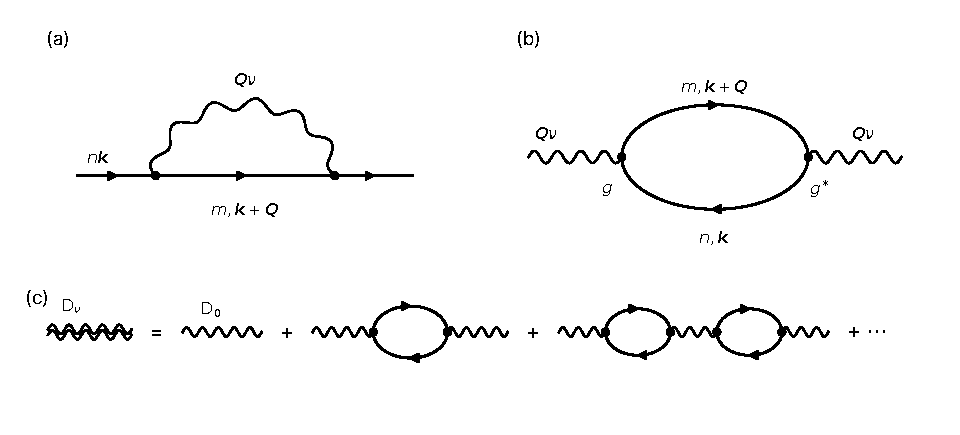
\includegraphics[width=\linewidth]{figures/ch06/fig6_5.pdf}
  \caption{The two second-order diagrams of the electron--phonon interaction. Solid lines with arrows are electrons, wavy lines phonons, dots the vertex $g$. (a) The electron self-energy: an electron in $(n,\vect{k})$ exchanges a phonon $(\vect{Q},\nu)$ with the intermediate state $(m,\vect{k}+\vect{Q})$. (b) The phonon self-energy: a phonon creates an electron in $(m,\vect{k}+\vect{Q})$ and a hole in $(n,\vect{k})$ through $g$, and the pair recombines through $g^*$. (c) The Dyson series for the dressed phonon propagator $\mathsf{D}_\nu$ (double wavy line): the free propagator $\mathsf{D}_0$ with any number of bubbles inserted.}
  \label{fig:6-bubble}
\end{figure}

The phonon Green's function in imaginary time is $\mathsf{D}_\nu(\vect{Q},\tau) = -\langle\mathrm{T}_\tau\,B_{\vect{Q}\nu}(\tau)\,B_{-\vect{Q}\nu}(0)\rangle$, with the free form $\mathsf{D}_0(\vect{Q}\nu,\ii\omega^{\mathrm{B}}_j) = 2\omega_{\vect{Q}\nu}/[(\ii\omega^{\mathrm{B}}_j)^2 - \omega_{\vect{Q}\nu}^2]$ of \cref{eq:D.11-D0}. Its expansion in $H_{\mathrm{ep}}$ is \cref{eq:D.11-Gexp} with $B_{\vect{Q}\nu}$ and $B_{-\vect{Q}\nu}$ as the external operators. The first nonzero correction is of second order. The expansion supplies $(-1)^2/2!$. The external $B_{\vect{Q}\nu}(\tau)$ is contracted with the boson of one of the two factors $H_{\mathrm{ep}}$, and $B_{-\vect{Q}\nu}(0)$ with the other; the two choices are equal after relabeling and cancel the $1/2!$. Each boson contraction is $-\mathsf{D}_0$. The vertex at $\tau_1$ must carry $B_{-\vect{Q}\nu}$, and the one at $\tau_2$ carries $B_{\vect{Q}\nu}$, so the vertices are $g_{mn\nu}(\vect{k},\vect{Q})^*$ and $g_{mn\nu}(\vect{k},\vect{Q})$ by \cref{eq:A.6-herm}, with the factor $1/N$ from the two $1/\sqrt N$. The two electron bilinears close into one loop, which gives $-1$ (rule 3 of \cref{app:D.11}) and a sum over two spin orientations. With the $-1$ of the definition, the total sign is $(-1)(-1)^2(-1) = +1$. In frequency space the correction is $\mathsf{D}_0\,\Pi^{\mathrm{b}}\,\mathsf{D}_0$ with
\begin{equation*}
  \Pi^{\mathrm{b}}_\nu(\vect{Q},\ii\omega^{\mathrm{B}}_j) = \frac2N\sum_{\vect{k}mn}|g_{mn\nu}(\vect{k},\vect{Q})|^2\;T\sum_{j'}\GF_0(n,\vect{k},\ii\omega^{\mathrm{F}}_{j'})\,\GF_0(m,\vect{k}+\vect{Q},\ii\omega^{\mathrm{F}}_{j'} + \ii\omega^{\mathrm{B}}_j) .
\end{equation*}
The frequency sum is \cref{eq:D.10-sum} with band labels, and
\begin{equation*}
  \Pi^{\mathrm{b}}_\nu(\vect{Q},\ii\omega^{\mathrm{B}}_j) = \frac2N\sum_{\vect{k}mn}|g_{mn\nu}(\vect{k},\vect{Q})|^2\,\frac{f_{n\vect{k}} - f_{m,\vect{k}+\vect{Q}}}{\ii\omega^{\mathrm{B}}_j + \varepsilon_{n\vect{k}} - \varepsilon_{m,\vect{k}+\vect{Q}}} .
\end{equation*}
Repeating the bubble along the phonon line gives the geometric series of \cref{fig:6-bubble}(c), $\mathsf{D} = \mathsf{D}_0 + \mathsf{D}_0\Pi^{\mathrm{b}}\mathsf{D}_0 + \dots = \mathsf{D}_0 + \mathsf{D}_0\Pi^{\mathrm{b}}\mathsf{D}$, so that $\mathsf{D}^{-1} = \mathsf{D}_0^{-1} - \Pi^{\mathrm{b}}$, a Dyson equation like \cref{eq:4.7-dyson} for electrons. With $\mathsf{D}_0^{-1} = [(\ii\omega^{\mathrm{B}}_j)^2 - \omega_{\vect{Q}\nu}^2]/2\omega_{\vect{Q}\nu}$ it is natural to define the self-energy in units of a squared frequency, $\Pi_\nu = 2\omega_{\vect{Q}\nu}\Pi^{\mathrm{b}}_\nu$. Continuing to $\omega + \ii0^+$,
\begin{keyresult}[Phonon self-energy and Dyson equation]
\begin{gather}
  \mathsf{D}_\nu(\vect{Q},\omega) = \frac{2\omega_{\vect{Q}\nu}}{\omega^2 - \omega_{\vect{Q}\nu}^2 - \Pi_\nu(\vect{Q},\omega)} , \notag\\
  \Pi_\nu(\vect{Q},\omega) = \frac{4\omega_{\vect{Q}\nu}}{N}\sum_{\vect{k}mn}|g_{mn\nu}(\vect{k},\vect{Q})|^2\,\frac{f_{n\vect{k}} - f_{m,\vect{k}+\vect{Q}}}{\omega + \varepsilon_{n\vect{k}} - \varepsilon_{m,\vect{k}+\vect{Q}} + \ii0^+} ,
  \label{eq:6.4-Pi}
\end{gather}
\end{keyresult}
with $f_{n\vect{k}} = n_{\mathrm{F}}(\xi_{n\vect{k}})$ the occupations and $\Pi_\nu$ in eV$^2$. The factor 4 is the 2 of $\mathsf{D}_0^{-1}$ times the two spin orientations of the loop. Note that we have put the screened vertex $g$ at both ends, with noninteracting electrons between them. Strictly, one end should carry the bare vertex~\cite[Eqs.~(145) and~(146)]{giustino2017electron}, which matters for the static part only. We have dropped the bubbles that connect two branches $\nu \ne \nu'$ at the same $\vect{Q}$. They mix the modes, and they matter where two branches are nearly degenerate.

The poles of $\mathsf{D}_\nu$ are the dressed phonons, $\omega^2 = \omega_{\vect{Q}\nu}^2 + \Pi_\nu(\vect{Q},\omega)$. When $|\Pi_\nu| \ll \omega_{\vect{Q}\nu}^2$ the root lies close to $\omega_{\vect{Q}\nu}$. Expanding the denominator there, $\omega^2 - \omega_{\vect{Q}\nu}^2 \simeq 2\omega_{\vect{Q}\nu}(\omega - \omega_{\vect{Q}\nu})$, turns $\mathsf{D}_\nu$ into a Lorentzian, $1/(\omega - \tilde\omega_{\vect{Q}\nu} + \ii\gamma_{\vect{Q}\nu}/2)$, with
\begin{equation}
  \tilde\omega_{\vect{Q}\nu} = \omega_{\vect{Q}\nu} + \frac{\Real\Pi_\nu(\vect{Q},\omega_{\vect{Q}\nu})}{2\omega_{\vect{Q}\nu}} , \qquad
  \gamma_{\vect{Q}\nu} = -\frac{\Imag\Pi_\nu(\vect{Q},\omega_{\vect{Q}\nu})}{\omega_{\vect{Q}\nu}} .
  \label{eq:6.4-pole}
\end{equation}
The real part shifts the phonon, and the imaginary part gives it a full width at half maximum $\gamma_{\vect{Q}\nu}$, the quantity of \cref{sec:5.7}. Its electron--phonon part is $\gamma^{\mathrm{ep}}_{\vect{Q}\nu}$, and the anharmonic bubble of \cref{sec:5.7} adds $\gamma^{\mathrm{anh}}_{\vect{Q}\nu}$ to it.

The sign of the static part is fixed. In an insulator at $T = 0$, $f_{n\vect{k}} - f_{m,\vect{k}+\vect{Q}} = +1$ for $n$ occupied and $m$ empty, and then $\varepsilon_{n\vect{k}} - \varepsilon_{m,\vect{k}+\vect{Q}} < 0$; the term with the roles exchanged has both signs reversed. Every term of $\Pi_\nu(\vect{Q},0)$ is therefore negative. The virtual pairs soften the lattice, as second-order perturbation theory always lowers a ground-state energy. In a metal the static bubble inherits the structure of the Lindhard function (\cref{sec:4.5}). For a spherical Fermi surface the density of pairs with $\varepsilon_{n\vect{k}} = \varepsilon_{m,\vect{k}+\vect{Q}} = E_{\mathrm{F}}$ changes abruptly when $Q$ passes $2k_{\mathrm{F}}$, the largest wavevector that joins two points of the surface, and the derivative of the Lindhard function diverges there logarithmically (\cref{app:C.8}). The phonon frequencies carry the singularity as a kink at $Q = 2k_{\mathrm{F}}$, or at whatever wavevectors span flat, parallel pieces of a real Fermi surface. This is the Kohn anomaly~\cite{kohn1959image}, and its position in a measured dispersion is an image of the Fermi surface.

\subsection{Adiabatic and nonadiabatic phonons}

The static part of $\Pi_\nu$ is already in the phonons we start from. Density-functional perturbation theory computes second derivatives of the Born--Oppenheimer energy with the electrons relaxed to their ground state at every nuclear configuration. The relaxation is the electronic response at zero frequency, which at this order is $\Pi_\nu(\vect{Q},0)$. The first-order density of \cref{eq:5.4-dn} is precisely that response, and the Hartree and exchange--correlation potential it generates is what turns the bare vertex at one end of the bubble into the screened one. Starting from the frequencies of such a calculation and adding the full $\Pi_\nu(\vect{Q},\omega)$ would count the static response twice. Only the difference between the dynamic and the static response may be added~\cite[Eqs.~(22) and~(23)]{calandra2010adiabatic},
\begin{equation}
  \bigl(\omega^{\mathrm{ren}}_{\vect{Q}\nu}\bigr)^2 = \omega_{\vect{Q}\nu}^2 + \Real\bigl[\Pi_\nu(\vect{Q},\omega^{\mathrm{ren}}_{\vect{Q}\nu}) - \Pi_\nu(\vect{Q},0)\bigr] ,
  \label{eq:6.4-nonad}
\end{equation}
where $\omega_{\vect{Q}\nu}$ is now the adiabatic frequency of density-functional perturbation theory and $\omega^{\mathrm{ren}}_{\vect{Q}\nu}$ the nonadiabatic one; this is the subtraction $W_e(\omega) - W_e(0)$ of Ref.~\cite[Eq.~(140)]{giustino2017electron}. The imaginary part needs no subtraction, since $\Pi_\nu(\vect{Q},0)$ is real.

How large is the remainder? In an insulator every denominator of \cref{eq:6.4-Pi} is at least $\Eg$ in magnitude, and the pair of terms with roles exchanged makes $\Pi_\nu$ even in $\omega$. The difference $\Pi_\nu(\omega) - \Pi_\nu(0)$ is then of relative order $(\omega_{\vect{Q}\nu}/\Eg)^2$, which is 0.003 for the optical phonon of silicon. The adiabatic phonons of an insulator are accurate, and this is the phonon-side statement of the counting of \cref{sec:6.1}, where $\omega_{\mathrm{ph}}/\Eg$ was the small parameter. A metal has no gap. Its intraband pairs with $|\varepsilon_{m,\vect{k}+\vect{Q}} - \varepsilon_{n\vect{k}}| \lesssim \omega_{\vect{Q}\nu}$ respond differently at $\omega = 0$ and at $\omega = \omega_{\vect{Q}\nu}$, and for them the difference is of order one. Such pairs dominate the bubble at small wavevector. For a band with Fermi velocity $v_{\mathrm{F}}$, the energy difference of a pair is $v_{\mathrm{F}}Q\cos\theta$, and the adiabatic and nonadiabatic frequencies differ appreciably only for $Q \lesssim \omega_{\vect{Q}\nu}/v_{\mathrm{F}}$~\cite{calandra2010adiabatic}. In aluminum, with $v_{\mathrm{F}} = \SI{2.0e6}{m.s^{-1}}$, that is $Q \lesssim \SI{2e-3}{\angstrom^{-1}}$ for a \SI{30}{meV} phonon, a thousandth of the zone. Near the zone center of metals with few carriers and stiff optical modes the correction can, however, be large. Calandra, Profeta and Mauri note corrections of up to \SI{30}{\percent} of the phonon frequency there~\cite{calandra2010adiabatic}; graphite intercalation compounds and doped graphene are the standard examples. Everywhere else the adiabatic frequencies are the right starting point.

The bubble with undressed vertices is itself an approximation. The counting of Migdal's theorem (\cref{sec:6.3}) makes the vertex corrections to it of relative order $\lambda_{\mathrm{ep}}\omega_{\mathrm{D}}/E_{\mathrm{F}}$, with the coupling constant $\lambda_{\mathrm{ep}}$ defined below; for aluminum, with phonon energies up to $\omega_{\max} = \SI{40}{meV}$ and $E_{\mathrm{F}} = \SI{11.7}{eV}$, that is at most 0.0015.

\subsection{The electron--phonon linewidth}

The width follows from the imaginary part of \cref{eq:6.4-Pi}. With $1/(x + \ii0^+) = \operatorname{PV}(1/x) - \ii\pi\delta(x)$ from \cref{eq:2.4-SP} in \cref{eq:6.4-pole},
\begin{keyresult}[Electron--phonon linewidth]
\begin{equation}
  \gamma^{\mathrm{ep}}_{\vect{Q}\nu} = -\frac{\Imag\Pi_\nu(\vect{Q},\omega_{\vect{Q}\nu})}{\omega_{\vect{Q}\nu}}
  = \frac{4\pi}{N}\sum_{\vect{k}mn}|g_{mn\nu}(\vect{k},\vect{Q})|^2\,\bigl(f_{n\vect{k}} - f_{m,\vect{k}+\vect{Q}}\bigr)\,\delta\bigl(\varepsilon_{m,\vect{k}+\vect{Q}} - \varepsilon_{n\vect{k}} - \omega_{\vect{Q}\nu}\bigr) ,
  \label{eq:6.4-gamma}
\end{equation}
\end{keyresult}
a full width, with the spin sum in the factor $4\pi = 2\times2\pi$. Ref.~\cite[Eq.~(146)]{giustino2017electron} writes the same rate as an inverse lifetime, with the spin factor 2 written explicitly, and its $1/\tau$ equals $\gamma^{\mathrm{ep}}_{\vect{Q}\nu}$. The cutting rule of \cref{sec:4.8} tells us how to read it. The delta function puts the pair on shell with the energy of the phonon, and $2\pi|g|^2/N$ times it is the golden-rule rate \cref{eq:2.5-golden} for absorbing the phonon into the pair $(n\vect{k} \to m,\vect{k}+\vect{Q})$. The occupation factor is the rate of that process, $f_n(1 - f_m)$, minus the rate of the inverse one, $f_m(1 - f_n)$, in which a pair recombines and emits the phonon; the difference is $f_n - f_m$.

In an undoped insulator at $T = 0$ the width vanishes below the gap. The delta function needs an occupied state $n$ and an empty state $m$ with $\varepsilon_m - \varepsilon_n = \omega_{\vect{Q}\nu}$, and every such difference is at least $\Eg$, while the largest phonon energy of silicon is \SI{64}{meV}. No term survives. The phonons of an insulator are, however, still broadened, by anharmonicity (\cref{sec:5.7}) and by isotopes and defects (\cref{sec:11.6}), which is why the measured \SI{0.18}{meV} width of the silicon Raman line could be compared with the three-phonon formula alone. At $T > 0$ thermally excited electrons and holes absorb phonons by intraband transitions, with a width proportional to their density, which in an intrinsic crystal is suppressed by $\ee^{-\Eg/2T}$: $4\times10^{-10}$ in silicon at room temperature. Doping supplies such carriers without the exponential, and a doped semiconductor behaves for this purpose like a dilute metal.

In a metal the electronic states near the Fermi level change on scales of eV, far larger than $\omega_{\vect{Q}\nu}$. For $T \ll E_{\mathrm{F}}$ the occupation difference at $\varepsilon_m = \varepsilon_n + \omega_{\vect{Q}\nu}$ is $f(\varepsilon_n) - f(\varepsilon_n + \omega_{\vect{Q}\nu}) \simeq -\omega_{\vect{Q}\nu}\,\partial f/\partial\varepsilon$, which tends to $\omega_{\vect{Q}\nu}\delta(\xi_{n\vect{k}})$ for $T \to 0$, and dropping $\omega_{\vect{Q}\nu}$ also in the remaining delta function, we arrive at Allen's formula~\cite{allen1972neutron},
\begin{equation}
  \gamma^{\mathrm{ep}}_{\vect{Q}\nu} \simeq \frac{4\pi\omega_{\vect{Q}\nu}}{N}\sum_{\vect{k}mn}|g_{mn\nu}(\vect{k},\vect{Q})|^2\,\delta(\xi_{n\vect{k}})\,\delta(\xi_{m,\vect{k}+\vect{Q}}) ,
  \label{eq:6.4-allen}
\end{equation}
which is positive term by term. Both electrons now sit on the Fermi surface, and the width is proportional to the phonon frequency. It no longer depends on temperature: thermal smearing removes states from below the Fermi level and adds them above, and the net number of pairs that can absorb $\omega_{\vect{Q}\nu}$ stays the same. The approximation requires bands that are smooth on the scale of $\omega_{\vect{Q}\nu}$ and a temperature small on the electronic scale. It fails for a band edge within $\omega_{\vect{Q}\nu}$ of the Fermi level, and for $Q \lesssim \omega_{\vect{Q}\nu}/v_{\mathrm{F}}$, the same small-$Q$ region where the nonadiabatic correction lives.

The electron gas makes the passage from \cref{eq:6.4-gamma} to \cref{eq:6.4-allen} explicit. For one parabolic band and a constant vertex, the angular integral in $(1/\Vol)\sum_{\vect{k}}(f_{\vect{k}} - f_{\vect{k}+\vect{Q}})\,\delta(\varepsilon_{\vect{k}+\vect{Q}} - \varepsilon_{\vect{k}} - \omega)$ gives $m_e/(kQ)$ wherever the delta function can be satisfied, and with $k\,\dd k = m_e\,\dd\varepsilon$ the radial integral becomes $\int\dd\varepsilon\,[f(\varepsilon) - f(\varepsilon + \omega)] = \omega$. The result, $m_e^2\omega/(4\pi^2Q)$ per spin and volume, holds at any $T \ll E_{\mathrm{F}}$ for $2k_{\mathrm{F}} > Q \gg \omega/v_{\mathrm{F}}$, and it is exactly what the double delta function of \cref{eq:6.4-allen} gives, $\omega\int\dd^3k\,(2\pi)^{-3}\delta(\xi_{\vect{k}})\,\delta(\xi_{\vect{k}+\vect{Q}}) = m_e^2\omega/(4\pi^2Q)$.

\subsection{The Eliashberg function}

The double sum in \cref{eq:6.4-allen} is a Fermi-surface average of $|g|^2$ for one phonon. Superconductivity, the electron mass enhancement and the resistivity of a metal all involve the same average, weighted over all phonons at a given energy. This weighted average is the Eliashberg function~\cite{eliashberg1960interactions},
\begin{equation}
  \alpha^2F(\omega) = \frac{1}{\mathcal{N}_{\mathrm{F}}\Omega\,N^2}\sum_{\vect{k}\vect{Q}}\sum_{mn\nu}|g_{mn\nu}(\vect{k},\vect{Q})|^2\,\delta(\xi_{n\vect{k}})\,\delta(\xi_{m,\vect{k}+\vect{Q}})\,\delta(\omega - \omega_{\vect{Q}\nu}) ,
  \label{eq:6.4-a2F}
\end{equation}
with $\mathcal{N}_{\mathrm{F}}$ the density of states per spin and volume at the Fermi level (\cref{sec:2.5}), so that $\mathcal{N}_{\mathrm{F}}\Omega$, per spin and per cell, satisfies $N\mathcal{N}_{\mathrm{F}}\Omega = \sum_{n\vect{k}}\delta(\xi_{n\vect{k}})$. The prefactor makes $\alpha^2F$ an average over initial states on the Fermi surface and a sum over final states, and it is dimensionless~\cite[Eq.~(205)]{giustino2017electron}. The symbol is read as one. If $|g|^2$ were the same for every pair on the Fermi surface, $\alpha^2F$ would be that constant times $\mathcal{N}_{\mathrm{F}}\Omega$ times the phonon density of states $g_{\mathrm{ph}}(\omega)$ of \cref{eq:5.2-dos}. The historical notation splits it this way into a coupling $\alpha^2(\omega)$ and a density $F(\omega)$. Comparing \cref{eq:6.4-allen,eq:6.4-a2F} term by term turns the Eliashberg function into a sum of linewidths, and it defines the coupling constant as its inverse moment~\cite[Eq.~(206)]{giustino2017electron}:
\begin{keyresult}[Eliashberg function, coupling constant and linewidths]
\begin{equation}
  \begin{gathered}
  \alpha^2F(\omega) = \frac{1}{4\pi\mathcal{N}_{\mathrm{F}}\Omega\,N}\sum_{\vect{Q}\nu}\frac{\gamma^{\mathrm{ep}}_{\vect{Q}\nu}}{\omega_{\vect{Q}\nu}}\,\delta(\omega - \omega_{\vect{Q}\nu}), \\
  \lambda_{\mathrm{ep}} = 2\int_0^\infty\dd\omega\,\frac{\alpha^2F(\omega)}{\omega} = \frac{1}{2\pi\mathcal{N}_{\mathrm{F}}\Omega\,N}\sum_{\vect{Q}\nu}\frac{\gamma^{\mathrm{ep}}_{\vect{Q}\nu}}{\omega_{\vect{Q}\nu}^2} .
  \end{gathered}
  \label{eq:6.4-lambda}
\end{equation}
\end{keyresult}
With a full width and a density of states per spin the factors are as written; a half width~\cite[Eq.~(185)]{giustino2017electron} or a two-spin $\mathcal{N}_{\mathrm{F}}$ changes them by factors of two. The coupling constant is a zone average of mode contributions $\lambda_{\vect{Q}\nu} = \gamma^{\mathrm{ep}}_{\vect{Q}\nu}/(2\pi\mathcal{N}_{\mathrm{F}}\Omega\,\omega_{\vect{Q}\nu}^2)$. We can therefore read the coupling of a mode off its measured linewidth, which was the point of Allen's relation~\cite{allen1972neutron}, and the factor $1/\omega^2$ makes soft modes with large widths dominate.

The name ``coupling constant'' comes from the electrons. Average the Fan--Migdal self-energy \cref{eq:6.3-FM} of a state $(n,\vect{k})$ over the Fermi surface, and insert $1 = \int\dd\omega'\,\delta(\omega' - \omega_{\vect{Q}\nu})\int\dd\varepsilon\,\delta(\varepsilon - \xi_{m,\vect{k}+\vect{Q}})$. Suppose that the density of final states and the vertices change little over the energy range $\omega_{\mathrm{D}}$ of the phonons. Then $\delta(\varepsilon - \xi_{m,\vect{k}+\vect{Q}})$ may be replaced by $\delta(\xi_{m,\vect{k}+\vect{Q}})$ under the average, and the weight of each $(\omega',\varepsilon)$ is $\alpha^2F(\omega')$ by \cref{eq:6.4-a2F}:
\begin{equation*}
  \langle\Sigma^{\mathrm{FM}}\rangle_{\mathrm{FS}}(\omega) = \int_0^\infty\dd\omega'\,\alpha^2F(\omega')\int_{-E_{\mathrm{band}}}^{E_{\mathrm{band}}}\dd\varepsilon\left[\frac{n_{\mathrm{B}}(\omega') + 1 - n_{\mathrm{F}}(\varepsilon)}{\omega - \varepsilon - \omega' + \ii0^+} + \frac{n_{\mathrm{B}}(\omega') + n_{\mathrm{F}}(\varepsilon)}{\omega - \varepsilon + \omega' + \ii0^+}\right] ,
\end{equation*}
where the cutoff $E_{\mathrm{band}} \gg \omega_{\mathrm{D}}$ is of the order of the band width. At $T = 0$ only $1 - \Theta(-\varepsilon) = \Theta(\varepsilon)$ survives in the first numerator and $\Theta(-\varepsilon)$ in the second. The $\varepsilon$ integrals are logarithms, $-\ln[(E_{\mathrm{band}} + \omega' - \omega)/(\omega' - \omega)]$ and $\ln[(E_{\mathrm{band}} + \omega' + \omega)/(\omega' + \omega)]$, whose derivatives at $\omega = 0$ are $-1/\omega' + 1/(E_{\mathrm{band}} + \omega')$ each and tend to $-1/\omega'$ for $E_{\mathrm{band}} \to \infty$; a finite band reduces each by the fraction $\omega'/(E_{\mathrm{band}} + \omega')$, \SI{1}{\percent} for $E_{\mathrm{band}} = 100\,\omega'$. The Allen--Heine term of \cref{eq:6.3-AH} does not depend on $\omega$ and does not contribute. The slope at the Fermi level is therefore $-2\int_0^\infty\dd\omega'\,\alpha^2F(\omega')/\omega'$, and by \cref{eq:6.4-lambda}
\begin{equation}
  -\frac{\partial\Real\langle\Sigma^{\mathrm{FM}}\rangle_{\mathrm{FS}}}{\partial\omega}\bigg|_{\omega=0} = \lambda_{\mathrm{ep}} .
  \label{eq:6.4-mass}
\end{equation}
By \cref{eq:4.7-qp} the quasiparticles within about $\omega_{\mathrm{D}}$ of the Fermi level have the residue $z_{\mathrm{qp}} = 1/(1 + \lambda_{\mathrm{ep}})$, their velocity is reduced by the same factor, and their density of states, and with it the electronic specific heat, is enhanced by $1 + \lambda_{\mathrm{ep}}$. The free electron gas has the specific heat $(\pi^2/3)\,2\mathcal{N}_{\mathrm{F}}\,T$ per volume~\cite[Chap.~2]{ashcroft1976solid}. For aluminum, for example, a density of states $2\mathcal{N}_{\mathrm{F}}\Omega = 5.49$ states per Ry and cell for both spins, computed from first principles~\cite[Table~II]{savrasov1996electron}, corresponds to \SI{0.951}{mJ.K^{-2}.mol^{-1}}, while the measured coefficient is \SI{1.36}{mJ.K^{-2}.mol^{-1}}~\cite[Table~II]{savrasov1996electron}. The ratio is $1 + \lambda_{\mathrm{ep}} = 1.43$. The specific heat alone measures $\lambda_{\mathrm{ep}} = 0.43$, without any phonon calculation.

The Eliashberg function has a different shape from the phonon density of states, and \cref{fig:6-a2F} shows by how much for aluminum. The model behind it is the simplest that still has the right ingredients. The phonons come from force constants between first and second neighbors of the fcc lattice, with $a = \SI{4.05}{\angstrom}$ and $M = \SI{26.98}{u}$. A neighbor at the lattice vector $\vect{R}$ contributes its spring tensor times $1 - \cos(\vect{Q}\cdot\vect{R})$ to the dynamical matrix, divided by $M$. The tensor of the first neighbor at $(a/2)(1,1,0)$ has the elements $0.648$ ($xx = yy$), $-0.187$ ($zz$) and $0.574$ ($xy$), and that of the second neighbor at $a(1,0,0)$ has $0.038$ ($xx$) and $-0.052$ ($yy = zz$), all in \si{eV.\angstrom^{-2}}. These five numbers are a least-squares fit to the measured zone-boundary frequencies, 9.69 and \SI{5.78}{THz} (longitudinal and transverse) at X and 9.69 and \SI{4.19}{THz} at L~\cite[Table~I]{savrasov1996electron}, and to the elastic constants $C_{11} = 106.8$, $C_{12} = 60.7$ and $C_{44} = \SI{28.2}{GPa}$ at a density of \SI{2.70}{g.cm^{-3}}~\cite{kittel2005introduction}, the room-temperature values of that source. They reproduce the transverse frequencies at X and L to \SI{2}{\percent} and the longitudinal one at L to \SI{8}{\percent}, and the largest phonon energy is \SI{40}{meV}.

The electrons are a free gas of three electrons per atom, with $k_{\mathrm{F}} = \SI{1.75}{\angstrom^{-1}}$ and $E_{\mathrm{F}} = \SI{11.7}{eV}$. The potential of each ion is a Coulomb potential $-3e^2/(4\pi r)$ outside a core radius $r_{\mathrm{c}}$ and zero inside, screened by the Lindhard function of \cref{sec:4.5}. Its Fourier transform per cell is $w(q) = -3e^2\cos(qr_{\mathrm{c}})/[\Omega q^2\varepsilon_{\mathrm{Lin}}(q,0)]$. For plane waves and one atom per cell, \cref{eq:A.6-g} becomes $g_\nu = (2M\omega_{\vect{Q}\nu})^{-1/2}(\vect{q}\cdot\vect{e}_\nu)\,w(q)$, where $\vect{q} = \vect{Q} + \vect{G}$ is the full momentum transfer, umklapp included. The sums over $\vect{k}$ and over the reciprocal-lattice vectors become integrals, $N^{-1}\sum_{\vect{k}} \to \Omega\int\dd^3k/(2\pi)^3$ and $N^{-1}\sum_{\vect{Q}}\sum_{\vect{G}} \to \Omega\int\dd^3q/(2\pi)^3$. The double delta function integrates to $\int\dd^3k\,(2\pi)^{-3}\delta(\xi_{\vect{k}})\delta(\xi_{\vect{k}+\vect{q}}) = m_e^2/(4\pi^2q)$ for $q < 2k_{\mathrm{F}}$, as for the linewidth of the electron gas, and with $\mathcal{N}_{\mathrm{F}} = m_ek_{\mathrm{F}}/2\pi^2$, \cref{eq:6.4-a2F} becomes
\begin{equation}
  \alpha^2F(\omega) = \frac{m_e\Omega}{2k_{\mathrm{F}}}\int_{q<2k_{\mathrm{F}}}\frac{\dd^3q}{(2\pi)^3}\sum_\nu\frac{(\hat{\vect{q}}\cdot\vect{e}_\nu)^2\,q\,|w(q)|^2}{2M\omega_{\vect{q}\nu}}\,\delta(\omega - \omega_{\vect{q}\nu}) .
  \label{eq:6.4-a2Fgas}
\end{equation}
The core radius is the only free parameter, a choice of the model. As a function of $r_{\mathrm{c}}$, $\lambda_{\mathrm{ep}}$ has a flat minimum at $r_{\mathrm{c}} = \SI{0.56}{\angstrom}$, where the zero of $\cos(qr_{\mathrm{c}})$ sits among the umklapp momentum transfers between $|\vect{G}_{111}| = \SI{2.69}{\angstrom^{-1}}$ and $2k_{\mathrm{F}} = \SI{3.50}{\angstrom^{-1}}$. We take $r_{\mathrm{c}}$ there, where the result depends least on it; between 0.55 and \SI{0.59}{\angstrom} the coupling stays between 0.44 and 0.46. The model uses no measured coupling.

\begin{figure}[t]
  \centering
  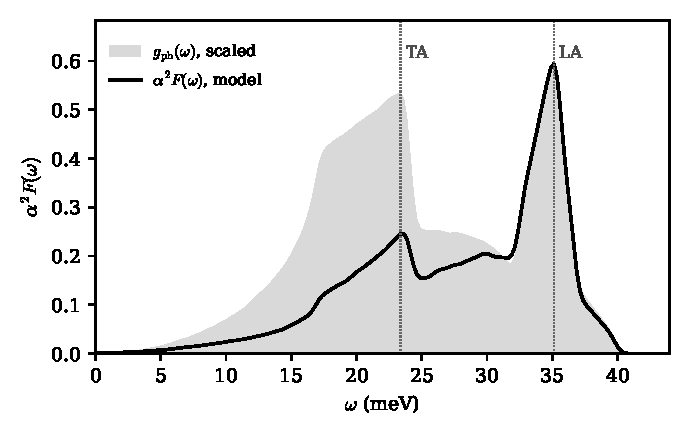
\includegraphics[width=0.75\linewidth]{figures/ch06/fig6_6.pdf}
  \caption{Eliashberg function of aluminum (black line) in a model of free electrons scattered by screened empty-core ions, \cref{eq:6.4-a2Fgas}, with the core radius, \SI{0.56}{\angstrom}, taken where $\lambda_{\mathrm{ep}}$ is stationary in it, with phonons from force constants between first and second neighbors fitted to measured zone-boundary frequencies and elastic constants. The gray area is the phonon density of states $g_{\mathrm{ph}}(\omega)$ of the same force constants, scaled to the height of the $\alpha^2F$ peak. Dotted lines mark the transverse (TA) and longitudinal (LA) maxima of $g_{\mathrm{ph}}$. In $\alpha^2F$ the transverse peak is suppressed, although three quarters of the modes lie below \SI{32}{meV}, because a transverse displacement couples to an electron only when the momentum transfer leaves the first zone. Both curves are histograms in bins of \SI{0.25}{meV} smoothed by a Gaussian of \SI{0.3}{meV}.}
  \label{fig:6-a2F}
\end{figure}

The result is $\lambda_{\mathrm{ep}} = 0.436$, against 0.44 from a linear-response calculation and 0.42 from tunneling spectra~\cite[Table~II]{savrasov1996electron}, and 0.43 from the specific heat above. Savrasov and Savrasov found their first-principles $\alpha^2F$ practically identical to an empirical rigid-ion pseudopotential result of this kind~\cite{savrasov1996electron}, and aluminum is the metal where the free-electron picture is expected to work. The shape carries more information than the number. Compared to the density of states, the transverse peak near \SI{23}{meV} is strongly suppressed. The reason is the factor $(\hat{\vect{q}}\cdot\vect{e}_\nu)^2$: within the first zone a transverse wave moves the ions perpendicular to $\vect{q}$, and an electron feels it only through an umklapp process, where $\vect{q} = \vect{Q} + \vect{G}$ has a component along the displacement. The logarithmic average frequency, $\omega_{\log} = \exp[(2/\lambda_{\mathrm{ep}})\int\dd\omega\,\alpha^2F(\omega)\ln\omega/\omega]$, which sets the prefactor of the critical temperature, comes out as \SI{250}{K}, against \SI{270}{K} from the linear-response calculation~\cite[Table~III]{savrasov1996electron}. A constant $\alpha^2$ with the same total weight would give 0.50 and \SI{228}{K}. Summed over the zone with \cref{eq:6.4-lambda}, the model widths average $\gamma^{\mathrm{ep}}_{\vect{Q}\nu}/\omega_{\vect{Q}\nu} = 4.4\times10^{-3}$ over all modes, or \SI{0.12}{meV}: a phonon in aluminum decays into electron--hole pairs after about 36 periods, much as the optical phonon of silicon decays anharmonically.

\begin{workedexample}{Coupling constant of aluminum from two Einstein peaks}\label{we:6-al}
Replace the model $\alpha^2F$ of \cref{fig:6-a2F} by two delta functions at the maxima of the phonon density of states, $\omega_{\mathrm{TA}} = \SI{23.4}{meV}$ and $\omega_{\mathrm{LA}} = \SI{35.1}{meV}$, each carrying the weight of $\alpha^2F$ on its side of the minimum of $g_{\mathrm{ph}}$ at \SI{31.9}{meV}. The weights are $I_{\mathrm{TA}} = \int_0^{31.9}\dd\omega\,\alpha^2F = \SI{3.13}{meV}$ and $I_{\mathrm{LA}} = \SI{2.26}{meV}$. Below the minimum lie 2.24 of the three modes per atom and above it 0.76, a ratio of 2.9; the weights of $\alpha^2F$ stand in the ratio 1.4, so each transverse mode couples half as strongly as a longitudinal one.

With $\alpha^2F = I_{\mathrm{TA}}\delta(\omega - \omega_{\mathrm{TA}}) + I_{\mathrm{LA}}\delta(\omega - \omega_{\mathrm{LA}})$, \cref{eq:6.4-lambda} gives
\begin{equation*}
  \lambda_{\mathrm{ep}} = 2\Bigl(\frac{I_{\mathrm{TA}}}{\omega_{\mathrm{TA}}} + \frac{I_{\mathrm{LA}}}{\omega_{\mathrm{LA}}}\Bigr) = 2\,(0.134 + 0.064) = 0.396 ,
\end{equation*}
\SI{9}{\percent} below the full model's 0.436 and 6 to \SI{8}{\percent} below the measured 0.42--0.43. The deficit is all in the transverse peak. The same weight spread over the low-frequency tail of \cref{fig:6-a2F} counts for more, since $1/\omega$ is convex, and the full transverse part is 0.306 instead of $2\times0.134 = 0.268$; the longitudinal part is 0.130 in both. Although the longitudinal peak is the taller, the transverse branches carry \SI{70}{\percent} of the coupling. For the two-peak model $\omega_{\log} = \exp[(2/\lambda_{\mathrm{ep}})(I_{\mathrm{TA}}\ln\omega_{\mathrm{TA}}/\omega_{\mathrm{TA}} + I_{\mathrm{LA}}\ln\omega_{\mathrm{LA}}/\omega_{\mathrm{LA}})] = \SI{26.7}{meV} = \SI{310}{K}$, too high for the same reason.
\end{workedexample}

In practice $\gamma^{\mathrm{ep}}_{\vect{Q}\nu}$ and $\alpha^2F$ are computed from \cref{eq:6.4-gamma,eq:6.4-a2F} with the vertices of density-functional perturbation theory, Wannier-interpolated to fine grids of $\vect{k}$ and $\vect{Q}$ as described in \cref{sec:6.2}. The two delta functions that pin both electrons to the Fermi surface make these the slowest-converging integrals of electron--phonon theory. \Cref{app:E.9} takes the resulting $\alpha^2F$ into the Eliashberg equations for the gap of aluminum, which come out at the measured \SI{0.18}{meV} once the Coulomb repulsion between paired electrons is fixed by the measured critical temperature.

The phonon-mediated attraction that binds those pairs is the exchange of the phonons whose widths we have just summed. \Cref{sec:7.2} reduces it to the model interaction of Bardeen, Cooper and Schrieffer, with $\lambda_{\mathrm{ep}}$ as its strength and $\omega_{\mathrm{D}}$ as its range in energy, and finds the gap that sets the threshold of a superconducting detector.

\section{Phonon-assisted optical absorption}\label{sec:6.5}

Silicon solar cells absorb the whole visible spectrum, from about 1.6 to \SI{3.3}{eV}, and silicon photodiodes respond down to its gap of \SI{1.17}{eV}. Yet the smallest vertical gap of silicon, $E_{\mathrm{dir}}$, is \SI{3.4}{eV} (\cref{sec:3.3}). A photon carries almost no crystal momentum, and on its own it can lift an electron only vertically, from $(v,\vect{k})$ to $(c,\vect{k})$. Every photon that silicon absorbs between \SI{1.17}{} and \SI{3.4}{eV} is therefore absorbed together with a phonon, which carries the crystal momentum $\vect{k}_{\mathrm{c}}$ from the valence maximum at $\mathrm{\Gamma}$ to a conduction valley. The phonon can be created or destroyed, and it takes a few tens of meV from the absorbed energy or adds as much. Phonon-assisted absorption is the simplest composite process: two vertices, the photon's and the electron--phonon vertex $g$ of \cref{sec:6.2}, joined through virtual intermediate states with the energy denominators of \cref{sec:2.4}. An absorbed dark-matter boson has even less momentum for its energy than a photon, and between the indirect and the direct gap it is absorbed only with a phonon (\cref{sec:13.8}). A scattering dark-matter particle just above its threshold mass delivers its energy at momentum transfers too small to reach $\vect{k}_{\mathrm{c}}$, and a phonon again supplies the crystal momentum that the momentum transfer lacks (\cref{sec:13.1}).

\subsection{The optical vertex}

A uniform optical field $\vect{\mathcal{E}}(t) = -\mathcal{E}\,\hat{\vect{e}}_\gamma\cos\omega t$, with unit polarization vector $\hat{\vect{e}}_\gamma$, is described by the vector potential $\vect{A}(t) = (\mathcal{E}/\omega)\,\hat{\vect{e}}_\gamma\sin\omega t$. To first order in $\vect{A}$ the field couples to the electrons through
\begin{equation}
  H_A = e\,\vect{A}\cdot\op{\vect{V}}, \qquad
  \op{\vect{V}} = \sum_{\vect{k}}\sum_{mn}\vect{v}_{mn}(\vect{k})\,c^\dagger_{m\vect{k}}c_{n\vect{k}} ,
  \label{eq:6.5-HA}
\end{equation}
where $\op{\vect{V}}$ is the total velocity of the electrons, written over Bloch states with the velocity matrix elements $\vect{v}_{mn}(\vect{k})$ of \cref{eq:3.2-pv}, and the spin is summed implicitly. For a local potential $\op{\vect{V}} = \sum_j\op{\vect{p}}_j/m_e$, and the sign of the charge is irrelevant for rates. The velocity operator conserves $\vect{k}$, because the velocity commutes with lattice translations. The part of $H_A$ that oscillates as $\ee^{-\ii\omega t}$ absorbs the energy $\omega$, with the amplitude $(e\mathcal{E}/2\omega)\,\hat{\vect{e}}_\gamma\cdot\op{\vect{V}}$ up to a phase.

\Cref{eq:6.5-HA} is the \emph{velocity form} of the optical vertex. Its alternative, the length form $e\vect{\mathcal{E}}\cdot\sum_j\vect{r}_j$, is awkward in a crystal, since the position has no matrix elements between extended Bloch states except through the commutator of \cref{eq:3.2-r}. The velocity form needs just $\vect{v} = \ii[H_{\mathrm{e}},\vect{r}]$, which stays well defined when the potential is nonlocal (\cref{eq:3.2-dHk}). It is also the vertex that dark matter shares with light. By \cref{eq:3.2-optical}, the density vertex at small momentum transfer is $\rho_{mn}(\vect{k},\vect{q}) \to \vect{q}\cdot\vect{v}_{mn}/(\varepsilon_{m\vect{k}} - \varepsilon_{n\vect{k}})$. On the energy shell the denominator is $\omega$, and a longitudinal field coupled through the density and a transverse field coupled through the velocity carry the same matrix element, $\hat{\vect{e}}_\gamma\cdot\vect{v}_{mn}/\omega$. Replacing the photon by dark matter replaces this optical limit by the full density vertex, and nothing else in the structure changes.

At first order the golden rule \cref{eq:2.5-golden} with $H_A$ gives the absorption rate between many-body states $i$ and $f$, and the absorbed power is $\omega$ times the net rate, absorption minus stimulated emission. Equating the time-averaged power per volume with $\sigma_1\mathcal{E}^2/2$ and using $\sigma_1 = \omega\varepsilon_2$ (\cref{eq:4.4-sigma}) gives
\begin{equation}
  \varepsilon_2(\omega) = \frac{\pi e^2}{\omega^2\Vol}\sum_{i,f}(p_i - p_f)\,\bigl|\hat{\vect{e}}_\gamma\cdot\langle f|\op{\vect{V}}|i\rangle\bigr|^2\,\delta(E_f - E_i - \omega) .
  \label{eq:6.5-eps2many}
\end{equation}
For independent electrons at $T \ll \Eg$ the final states are one electron in $(c,\vect{k})$ and one hole in $(v,\vect{k})$, and \cref{eq:6.5-eps2many} is the direct absorption of \cref{sec:4.4}, the familiar sum over vertical transitions,
\begin{equation}
  \varepsilon_2(\omega) = \frac{g_{\mathrm{deg}}\,\pi e^2}{\omega^2 \Vol}\sum_{\vect{k}}\sum_{cv}\bigl|\hat{\vect{e}}_\gamma\cdot\vect{v}_{cv}(\vect{k})\bigr|^2\,\delta(\varepsilon_{c\vect{k}} - \varepsilon_{v\vect{k}} - \omega) ,
  \label{eq:6.5-eps2dir}
\end{equation}
with $g_{\mathrm{deg}} = 2$ for the spin~\cite[Chap.~6]{yu2010fundamentals}. In a frozen lattice this direct $\varepsilon_2$ vanishes below $E_{\mathrm{dir}}$, and below $E_{\mathrm{dir}}$ light needs something else to supply the crystal momentum. A phonon can, and so can an impurity or a free carrier; in a pure, cold crystal only the phonon remains. The absorption coefficient, the inverse length over which the intensity falls by $\ee$, follows from $\varepsilon_2$ and the refractive index $n_r(\omega)$ as
\begin{equation}
  \alpha_{\mathrm{abs}}(\omega) = \frac{\omega\,\varepsilon_2(\omega)}{n_r(\omega)} ,
  \label{eq:6.5-alpha}
\end{equation}
since, with $\varepsilon = (n_r + \ii\kappa_{\mathrm{ext}})^2$ and $\kappa_{\mathrm{ext}}$ the extinction coefficient, the intensity decays as $\ee^{-2\omega\kappa_{\mathrm{ext}}x}$ and $\varepsilon_2 = 2n_r\kappa_{\mathrm{ext}}$.

\subsection{The phonon-assisted amplitude}

Add the electron--phonon Hamiltonian $H_{\mathrm{ep}}$ of \cref{eq:A.6-Hep} and count the phonons in the states. The initial state $|i\rangle$ has filled valence bands, empty conduction bands and $n_{\vect{Q}\nu}$ phonons in each mode. The final state has an electron in $(c,\vect{k}+\vect{Q})$, a hole in $(v,\vect{k})$, and one phonon fewer in the mode $(\vect{Q},\nu)$ or one more in $(-\vect{Q},\nu)$. No single vertex connects the initial and the final state. $H_A$ conserves $\vect{k}$ and does not touch the phonons, and $H_{\mathrm{ep}}$ changes $\vect{k}$ but cannot create a pair across a gap of an electronvolt with tens of meV. The second-order amplitude of \cref{eq:2.4-c2}, linear in $H_A$ and linear in $H_{\mathrm{ep}}$, both changes $\vect{k}$ and creates the pair. Its long-time limit is the rate $2\pi|T_{fi}|^2\delta(E_f - E_i - \omega)$ of \cref{eq:2.4-golden2}, with the two time orderings of \cref{eq:2.4-orderings}:
\begin{equation*}
  T_{fi} = \frac{e\mathcal{E}}{2\omega}\sum_m\left[\frac{\langle f|H_{\mathrm{ep}}|m\rangle\langle m|\hat{\vect{e}}_\gamma\cdot\op{\vect{V}}|i\rangle}{E_i + \omega - E_m} + \frac{\langle f|\hat{\vect{e}}_\gamma\cdot\op{\vect{V}}|m\rangle\langle m|H_{\mathrm{ep}}|i\rangle}{E_i - E_m}\right] .
\end{equation*}
The photon energy appears in the denominator of the photon-first ordering, where it has been absorbed in the intermediate state, and not in the phonon-first one.

Four kinds of intermediate state contribute; we drop the common factors $e\mathcal{E}/2\omega$, $N^{-1/2}$ from \cref{eq:A.6-Hep} and the phonon matrix element $(n_{\vect{Q}\nu} + \frac12 \pm \frac12)^{1/2}$ of \cref{eq:A.6-weights}, with the upper sign for emission throughout.
\begin{enumerate}
  \item The photon lifts the electron from $(v,\vect{k})$ to an empty state $(p,\vect{k})$, and the phonon scatters it to $(c,\vect{k}+\vect{Q})$. The intermediate energy exceeds $E_i + \omega$ by $\varepsilon_{p\vect{k}} - \varepsilon_{v\vect{k}} - \omega$. The operator string is $c^\dagger_cc_p\,c^\dagger_pc_v$, and since $p$ is empty it equals $c^\dagger_cc_v$. The term is $g_{cp\nu}(\vect{k},\vect{Q})\hat{\vect{e}}_\gamma\cdot\vect{v}_{pv}(\vect{k})/(\omega - \varepsilon_{p\vect{k}} + \varepsilon_{v\vect{k}})$.
  \item The phonon scatters the electron from $(v,\vect{k})$ to an empty $(p,\vect{k}+\vect{Q})$, and the photon lifts it to $(c,\vect{k}+\vect{Q})$. The intermediate state holds the pair and the changed phonon, $E_m - E_i = \varepsilon_{p,\vect{k}+\vect{Q}} - \varepsilon_{v\vect{k}} \pm \omega_{\vect{Q}\nu}$, and the term is $\hat{\vect{e}}_\gamma\cdot\vect{v}_{cp}(\vect{k}+\vect{Q})\,g_{pv\nu}(\vect{k},\vect{Q})/(\varepsilon_{v\vect{k}} - \varepsilon_{p,\vect{k}+\vect{Q}} \mp \omega_{\vect{Q}\nu})$.
  \item The photon creates the electron in $(c,\vect{k}+\vect{Q})$ from an occupied $(p,\vect{k}+\vect{Q})$, and the phonon then moves an electron from $(v,\vect{k})$ into the hole. The string $c^\dagger_pc_v\,c^\dagger_cc_p$ reorders to $-c^\dagger_c\,c^\dagger_pc_p\,c_v$, which is $-c^\dagger_cc_v$ on a state with $p$ occupied. The term is $-\hat{\vect{e}}_\gamma\cdot\vect{v}_{cp}(\vect{k}+\vect{Q})\,g_{pv\nu}(\vect{k},\vect{Q})/(\omega - \varepsilon_{c,\vect{k}+\vect{Q}} + \varepsilon_{p,\vect{k}+\vect{Q}})$.
  \item The phonon creates the electron in $(c,\vect{k}+\vect{Q})$ from an occupied $(p,\vect{k})$, and the photon moves an electron from $(v,\vect{k})$ into the hole. The same reordering gives $-1$, and the term is $-g_{cp\nu}(\vect{k},\vect{Q})\hat{\vect{e}}_\gamma\cdot\vect{v}_{pv}(\vect{k})/(\varepsilon_{p\vect{k}} - \varepsilon_{c,\vect{k}+\vect{Q}} \mp \omega_{\vect{Q}\nu})$.
\end{enumerate}
In the first two paths the electron propagates in the intermediate state, in the last two the hole; the hole paths are the Z graphs of old-fashioned perturbation theory. \Cref{fig:6-orderings} draws the two electron paths for silicon. Near the absorption edge of silicon, with $\omega \approx \Eg$ and the lowest vertical transition at \SI{3.4}{eV}, the intermediate electron of path 1 is off the energy shell by about \SI{2}{eV}. In silicon the natural intermediate state of path 2 is a valence state at $\vect{k}_{\mathrm{c}}$, which is occupied. The electron cannot enter a band $p$ that is already full; \cref{sec:2.4} anticipated this Pauli blocking, and paths 3 and 4 take the place of path 2.

\begin{figure}[tbp]
  \centering
  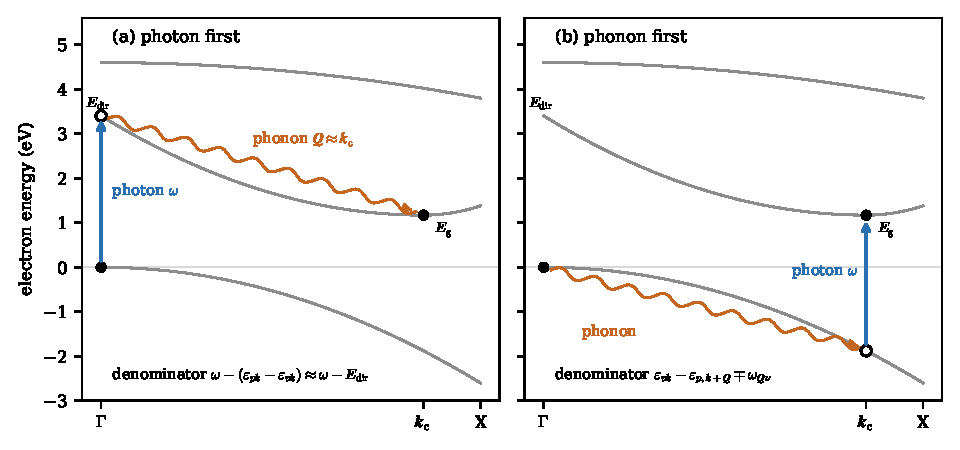
\includegraphics[width=\linewidth]{figures/ch06/fig6_7.pdf}
  \caption{The two time orderings of phonon-assisted absorption across the indirect gap of silicon, on schematic bands along $\mathrm{\Gamma}$--X. Filled dots: the initial electron at the valence maximum at $\mathrm{\Gamma}$ and the final electron at the conduction minimum near $\vect{k}_{\mathrm{c}} = 0.85\,(2\pi/a)$, \SI{1.17}{eV} higher. Open dots: virtual intermediate states. Straight arrows: the vertical optical vertex $\hat{\vect{e}}_\gamma\cdot\vect{v}$; wavy arrows: the electron--phonon vertex $g$, which changes the crystal momentum by $\vect{Q} \approx \vect{k}_{\mathrm{c}}$ and the energy by just $\pm\omega_{\vect{Q}\nu}$, tens of meV. Energy is not conserved at the intermediate state; each panel gives the energy denominator with which its amplitude enters \cref{eq:6.5-M}. (a) Photon first: the intermediate electron is at $\mathrm{\Gamma}$, and the denominator vanishes when $\omega$ reaches the vertical gap $E_{\mathrm{dir}} = \SI{3.4}{eV}$. (b) Phonon first: the intermediate state is a valence state at $\vect{k}_{\mathrm{c}}$, which is occupied. The process then runs through hole orderings, in which an electron from an occupied band is promoted first and the valence electron fills the hole it leaves (sign $-1$), and the denominator of these orderings never vanishes. Band curves drawn by hand; only $\Eg$, $E_{\mathrm{dir}}$ and $\vect{k}_{\mathrm{c}}$ are measured values.}
  \label{fig:6-orderings}
\end{figure}

On the energy shell, $\omega = \varepsilon_{c,\vect{k}+\vect{Q}} - \varepsilon_{v\vect{k}} \pm \omega_{\vect{Q}\nu}$, the denominator of path 3 becomes $\varepsilon_{p,\vect{k}+\vect{Q}} - \varepsilon_{v\vect{k}} \pm \omega_{\vect{Q}\nu}$, and its term takes the form of path 2 with an occupied $p$. The denominator of path 4 becomes $\varepsilon_{p\vect{k}} - \varepsilon_{v\vect{k}} - \omega$, and its term takes the form of path 1 with an occupied $p$. The fermion sign of the hole paths is what makes their terms match the electron paths. The four paths therefore combine into a single one-electron amplitude, summed over every band $p$, occupied or empty:
\begin{equation}
  M^{\pm}_{cv\nu}(\vect{k},\vect{Q}) = \sum_p\left[\frac{g_{cp\nu}(\vect{k},\vect{Q})\;\hat{\vect{e}}_\gamma\cdot\vect{v}_{pv}(\vect{k})}{\omega - \varepsilon_{p\vect{k}} + \varepsilon_{v\vect{k}}} + \frac{\hat{\vect{e}}_\gamma\cdot\vect{v}_{cp}(\vect{k}+\vect{Q})\;g_{pv\nu}(\vect{k},\vect{Q})}{\varepsilon_{v\vect{k}} - \varepsilon_{p,\vect{k}+\vect{Q}} \mp \omega_{\vect{Q}\nu}}\right] .
  \label{eq:6.5-M}
\end{equation}
The sum includes $p = v$ and $p = c$, in which the photon acts as an intraband velocity and the phonon does all the interband work. Refs.~\cite[Eq.~(200)]{giustino2017electron} and~\cite[Eqs.~(2) and~(3)]{noffsinger2012phonon} write the same sum with both denominators of opposite sign, a change that leaves $|M^\pm|^2$ unchanged. Note that the phonon energy enters twice: in the denominator of the phonon-first term, where against electronic energies of electronvolts it is usually negligible, and in the energy balance $\omega = \varepsilon_{c,\vect{k}+\vect{Q}} - \varepsilon_{v\vect{k}} \pm \omega_{\vect{Q}\nu}$, where it shifts the threshold.

A rough size of the amplitude follows from \cref{eq:6.5-M} before any calculation. Compared to a direct transition with a velocity matrix element of similar size, the phonon-assisted amplitude carries an extra factor of the vertex over a denominator. Typical optical-phonon vertices in silicon are a few tenths of an eV (\cref{sec:6.2}) and the denominators near the silicon edge are 2 to \SI{3}{eV}; together they put $|M^\pm|^2$ at $\sim10^{-2}$ of the squared optical vertex for each phonon mode that couples. The phonon-assisted $\varepsilon_2$ near the indirect edge is then $\sim10^{-2}$ of the direct one above $E_{\mathrm{dir}}$, before phase space and occupations are counted. This factor of $\sim10^{-2}$ is why silicon absorbs weakly between its two gaps, and why, for dark matter, the phonon-assisted rate dominates only where the zero-phonon rate is kinematically forbidden.

The photon-first denominator vanishes when $\omega = \varepsilon_{p\vect{k}} - \varepsilon_{v\vect{k}}$, that is, when the photon alone could create a real pair at $\vect{k}$. In silicon the denominator first vanishes at $E_{\mathrm{dir}}$. There the intermediate electron becomes real, and \cref{sec:2.4} gives the treatment. A real electron decays, by phonon emission among other channels, with a width $\varGamma_{\mathrm{w}}$ (\cref{sec:6.3}), and the denominator acquires $+\ii\varGamma_{\mathrm{w}}/2$ (\cref{eq:2.4-width}). By \cref{eq:2.4-split} the squared resonant term then splits into an on-shell part and a finite part. The on-shell part is a cascade: direct absorption at $\vect{k}$, followed by the scattering of the real electron by a phonon, weighted by the branching ratio of the phonon scattering. Direct absorption already counts the cascade once, in \cref{eq:6.5-eps2dir} with a broadened delta function. Adding the full phonon-assisted $\varepsilon_2$ to the direct one above $E_{\mathrm{dir}}$ counts the cascade twice. Below $E_{\mathrm{dir}}$ the double counting does not arise: every intermediate state is off shell, by electronvolts at the indirect edge. First-principles calculations in silicon give the intermediate states a constant width of \SI{100}{meV} and find the spectrum between the gaps insensitive to this width~\cite{noffsinger2012phonon}; the insensitivity is the numerical form of the statement that every intermediate state is off shell.

\subsection{The phonon-assisted dielectric function}

The rest of the derivation is bookkeeping, done as for \cref{eq:6.5-eps2dir}: $T_{fi}$ goes into the rate, the rate into the absorbed power, and the power into $\varepsilon_2$. Summing over the final states, labeled by $\vect{k}$, $\vect{Q}$, $\nu$, $c$, $v$, the spin and the sign, we obtain
\begin{keyresult}[Phonon-assisted dielectric function]
\begin{equation}
  \varepsilon_2^{\mathrm{PA}}(\omega) = \frac{g_{\mathrm{deg}}\,\pi e^2}{\omega^2\,\Omega}\,\Bigl\langle\!\Bigl\langle\sum_{\nu}\sum_{cv}\sum_\pm\bigl(n_{\vect{Q}\nu} + \tfrac12 \pm \tfrac12\bigr)\,\bigl|M^{\pm}_{cv\nu}(\vect{k},\vect{Q})\bigr|^2\,\delta\bigl(\varepsilon_{c,\vect{k}+\vect{Q}} - \varepsilon_{v\vect{k}} \pm \omega_{\vect{Q}\nu} - \omega\bigr)\Bigr\rangle\!\Bigr\rangle ,
  \label{eq:6.5-eps2PA}
\end{equation}
\end{keyresult}
where $\langle\!\langle\cdots\rangle\!\rangle$ is the average over the electron wavevector $\vect{k}$ and the phonon wavevector $\vect{Q}$ in the zone of \cref{eq:A.3-BZ}, and $g_{\mathrm{deg}} = 2$ counts the spin. The formula holds for $T \ll \Eg$, where thermally excited pairs, which would run the process backwards, are absent. Together with \cref{eq:6.5-alpha}, \cref{eq:6.5-eps2PA} gives the absorption coefficient used in first-principles work. Ref.~\cite[Eq.~(1)]{noffsinger2012phonon} writes it in Gaussian units, $e_{\mathrm{G}}^2 = e^2/4\pi$ (\cref{app:A.2}), with the spin factor explicit, and Ref.~\cite[Eq.~(200)]{giustino2017electron} writes it with the spin sum implicit. \Cref{eq:6.5-eps2PA} adds to the direct $\varepsilon_2$ of \cref{eq:6.5-eps2dir}, and below $E_{\mathrm{dir}}$ it is the whole absorption.

The formula contains three sums, and each sets a cost. The sum over intermediate bands $p$, inside $M^\pm$, runs over occupied and empty bands alike, and it converges no faster than its denominators grow; a calculation must include bands several electronvolts above the conduction minimum. The sum over phonon branches is short, six in silicon. The average over $\vect{k}$ and $\vect{Q}$ is the expensive one. The two wavevectors range independently over the whole zone, linked by the energy delta function alone, and the onset region needs both on fine grids. An energy resolution of \SI{14}{meV} in silicon took $40^3$ points for each, $4\times10^9$ pairs, each with its own vertices for every pair of bands~\cite{noffsinger2012phonon}.

In practice no calculation computes so many vertices directly. The energies, velocities and vertices are computed by density-functional perturbation theory on coarse grids, rotated to Wannier functions, and interpolated to the fine grids, with every quantity in one gauge (\cref{sec:6.2}). Two corrections enter the optical vertex. With a nonlocal pseudopotential the velocity includes the commutator of the nonlocal part (\cref{eq:3.2-dHk}), and when the gap is corrected the velocities are rescaled by the ratio of corrected to Kohn--Sham transition energies (\cref{eq:E.3-vrescale}). A different route avoids the double sum altogether. Freezing the nuclei of a supercell in a special displaced configuration breaks translation symmetry; the photon then connects states of different crystal momentum, and one static calculation of $\varepsilon_2$ in that supercell contains the phonon-assisted absorption at a given temperature (\cref{sec:6.3}). Being adiabatic, the special-displacement calculation does not distinguish the emission of a phonon from its absorption, and it cannot resolve the two thresholds $\Eg \pm \omega_{\vect{Q}\nu}$ that the next subsection derives.

\subsection{The Hall--Bardeen--Blatt edge}

Just above the threshold, \cref{eq:6.5-eps2PA} simplifies enough to be done by hand. The final hole lies near the valence maximum at $\vect{k} = 0$, and the final electron near one of the conduction minima $\vect{k}_{\mathrm{c}}$. We measure their crystal momenta from the extrema, $\vect{k} = \vect{\kappa}_{\mathrm{h}}$ and $\vect{k} + \vect{Q} = \vect{k}_{\mathrm{c}} + \vect{\kappa}_{\mathrm{e}}$, and take the bands as parabolic, with kinetic energies $E_{\mathrm{h}} = \kappa_{\mathrm{h}}^2/2m_{\mathrm{h}}$ and $E_{\mathrm{e}} = \kappa_{\mathrm{e}}^2/2m^*_{\mathrm{d}}$. Here $m_{\mathrm{h}}$ is the mass of one valence band and $m^*_{\mathrm{d}} = (m^*_\parallel m^{*2}_\perp)^{1/3}$ the density-of-states mass of one valley, $0.322\,m_e$ in silicon with the valley masses of \cref{tab:3-materials}. Two approximations make the sums elementary. First, the phonon wavevector $\vect{Q} = \vect{k}_{\mathrm{c}} + \vect{\kappa}_{\mathrm{e}} - \vect{\kappa}_{\mathrm{h}}$ stays within the small pockets around $\vect{k}_{\mathrm{c}}$, and the phonon energies and vertices may be taken at $\vect{Q} = \vect{k}_{\mathrm{c}}$; we write $\omega_\nu \equiv \omega_{\vect{k}_{\mathrm{c}}\nu}$ and $n_\nu = n_{\mathrm{B}}(\omega_\nu)$. Second, the denominators of \cref{eq:6.5-M} are electronic energy differences of an electronvolt or more, far from any resonance, and they barely change across the pockets. The squared amplitude $|M^\pm|^2$ is then a constant, its value $|M^\pm_\nu|^2$ at the extrema.

Then only phase space remains. The averages over $\vect{k}$ and $\vect{Q}$ become independent integrals over $\vect{\kappa}_{\mathrm{h}}$ and $\vect{\kappa}_{\mathrm{e}}$, each of which turns into an energy integral with the density of states of a parabolic band, $\int\dd^3\kappa\,(2\pi)^{-3} = \int\dd E\,(2m)^{3/2}E^{1/2}/4\pi^2$. The delta function fixes $E_{\mathrm{e}} + E_{\mathrm{h}} = x$, the energy above the threshold, and
\begin{equation}
  \begin{aligned}
  \Omega^2\!\int\!\frac{\dd^3\kappa_{\mathrm{h}}}{(2\pi)^3}\frac{\dd^3\kappa_{\mathrm{e}}}{(2\pi)^3}\,\delta(x - E_{\mathrm{e}} - E_{\mathrm{h}})
  &= \frac{\Omega^2\,(2m^*_{\mathrm{d}})^{3/2}(2m_{\mathrm{h}})^{3/2}}{16\pi^4}\int_0^x\dd E_{\mathrm{e}}\,E_{\mathrm{e}}^{1/2}(x - E_{\mathrm{e}})^{1/2}\\
  &= \frac{\Omega^2\,(m^*_{\mathrm{d}}m_{\mathrm{h}})^{3/2}}{16\pi^3}\,x^2 ,
  \end{aligned}
  \label{eq:6.5-joint}
\end{equation}
for $x \ge 0$, since the last integral is $\pi x^2/8$. Two densities of states, each growing as $\varepsilon^{1/2}$, have a convolution that grows as $x^2$. A direct edge has one free momentum, because the photon ties the electron to the hole, and its joint density of states grows as $x^{1/2}$; the phonon frees the second momentum and adds a power $3/2$. With all factors collected, each valley, valence band and branch adds a term
\begin{keyresult}[Hall--Bardeen--Blatt edge]
\begin{equation}
  \begin{aligned}
  \alpha_{\mathrm{abs}}(\omega) \simeq \sum_\nu A_\nu\Bigl[&n_\nu\,(\omega - \Eg + \omega_\nu)^2\,\Theta(\omega - \Eg + \omega_\nu)\\
  &+ (n_\nu + 1)\,(\omega - \Eg - \omega_\nu)^2\,\Theta(\omega - \Eg - \omega_\nu)\Bigr] ,
  \end{aligned}
  \label{eq:6.5-edge}
\end{equation}
\end{keyresult}
with
\begin{equation*}
  A_\nu = \frac{g_{\mathrm{deg}}\,e^2\,\Omega\,(m^*_{\mathrm{d}}m_{\mathrm{h}})^{3/2}}{16\pi^2\,\omega\,n_r}\,\sum_{\text{valleys}}|M_\nu|^2 ,
\end{equation*}
constant across the edge. In $A_\nu$ we have set $|M^+_\nu| = |M^-_\nu| \equiv |M_\nu|$, which holds when $\omega_\nu$ is negligible in the denominators, and treated $\omega$ and $n_r$ as constant over the width of the edge, a few times $\omega_\nu$ or about \SI{0.1}{eV}. Heavy and light holes enter as separate valence bands, each with its own $m_{\mathrm{h}}$. \Cref{eq:6.5-edge} is the form of Hall, Bardeen and Blatt~\cite{hall1954infrared}.

\Cref{eq:6.5-edge} turns the edge into a spectroscopy. Each branch that couples contributes two components with the same coefficient $A_\nu$: one starting at $\Eg - \omega_\nu$, where the photon is helped by a phonon absorbed from the lattice, and one at $\Eg + \omega_\nu$, where a phonon is emitted. The midpoint of each pair of thresholds is $\Eg$, and their separation is $2\omega_\nu$. Each component is a straight line in a plot of $\sqrt{\alpha_{\mathrm{abs}}}$ against $\omega$, with slope $\sqrt{A_\nu n_\nu}$ or $\sqrt{A_\nu(n_\nu + 1)}$. The sum of several components is not a straight line, and the measured curve is decomposed by subtracting, at each threshold, the extrapolation of the components that started below it.

The quadratic law assumes that $M_\nu$ is finite at the extrema, that is, that the transition is \emph{allowed} there. If symmetry forces $M_\nu$ to vanish at the extrema, it grows linearly with $\kappa_{\mathrm{e}}$ or $\kappa_{\mathrm{h}}$, an extra power of energy enters the integrand of \cref{eq:6.5-joint}, and the forbidden edge grows as $x^3$. The quadratic law also neglects the attraction between the electron and the hole. In silicon the bound pair, the exciton, lies $E_x^b = \SI{14.7}{meV}$ below the gap at total crystal momentum $\vect{k}_{\mathrm{c}}$ (\cref{sec:4.9}), and a photon reaches the exciton with a phonon just as it reaches a free pair. Each threshold of \cref{eq:6.5-edge} therefore has an excitonic companion $E_x^b$ lower, with its own onset shape, and the kinks of a measured edge are exciton thresholds at $\Eg - E_x^b \pm \omega_\nu$.

\subsection{Temperature dependence}

All of the temperature dependence of \cref{eq:6.5-edge} at a fixed gap is in the occupations. The component that absorbs a phonon is proportional to $n_\nu$, the number of phonons available; the one that emits is proportional to $n_\nu + 1$, spontaneous plus stimulated emission. Their ratio,
\begin{equation}
  \frac{n_\nu}{n_\nu + 1} = \ee^{-\omega_\nu/T} ,
  \label{eq:6.5-ratio}
\end{equation}
is detailed balance (\cref{eq:2.5-db}) for the phonon system alone: the two components have the same $|M_\nu|^2$, and the lattice gives up an energy $\omega_\nu$ with a Boltzmann penalty relative to taking it. The ratio of the slopes of the two components in $\sqrt{\alpha_{\mathrm{abs}}}$ is $\ee^{-\omega_\nu/2T}$, and the edge is a thermometer of the lattice that needs no knowledge of $A_\nu$. At high temperature both components grow as $T/\omega_\nu$, and the total weight of a branch, proportional to $2n_\nu + 1$, rises with $T$.

As $T \to 0$ the absorption components vanish. A cold crystal has no phonons to give, and every photon absorbed at the indirect edge must create one. The edge then lies at $\Eg + \omega_\nu$ for the softest branch that couples, and the energy $\omega_\nu$ of the emitted phonon goes into the lattice, not into the pair. At the \SI{10}{mK} of a dark-matter detector the emission-only edge is exact for every practical purpose: the transverse-acoustic occupation in silicon is vanishingly small (\cref{we:6-siedge}).

The gap itself also moves with temperature. The phonon-assisted formula contains the occupations explicitly; the bands in \cref{eq:6.5-eps2PA} are the bands the electrons actually occupy, renormalized by the same electron--phonon coupling (\cref{sec:6.3}). In silicon the gap shrinks from \SI{1.17}{eV} at low temperature to \SI{1.12}{eV} at \SI{300}{K} (\cref{sec:3.3}), and all four thresholds of each branch move down with it. First-principles spectra that include the occupations alone must be shifted rigidly to match the measured onsets, by 0.15 to \SI{0.23}{eV} in silicon, a shift that absorbs both the remaining error of the computed gap and the electron--phonon renormalization of the gap~\cite{noffsinger2012phonon}.

\subsection{The silicon edge}

Macfarlane, McLean, Quarrington and Roberts measured the absorption edge of silicon between \SI{4.2}{} and \SI{415}{K}, with enough resolution to see the thresholds of \cref{eq:6.5-edge}~\cite{macfarlane1958fine}. They found four series of thresholds and quoted the phonon energies as temperatures $\theta$, which in natural units are the energies themselves. Two of these phonon energies, $\theta = \SI{212}{K}$ and \SI{670}{K}, belong to the transverse-acoustic and transverse-optical phonons at $\vect{k}_{\mathrm{c}}$~\cite[Chap.~6]{yu2010fundamentals}. With $\SI{1}{K} = \SI{86.17}{\micro eV}$ (\cref{sec:2.5}) the two energies are
\begin{equation*}
  \omega_{\mathrm{TA}} = \SI{18.27}{meV}, \qquad \omega_{\mathrm{TO}} = \SI{57.73}{meV} .
\end{equation*}
Neutron scattering measures the same branches at the zone boundary X, at \SI{4.49}{THz} and \SI{13.90}{THz}, or \SI{18.57}{meV} and \SI{57.49}{meV} (\cref{sec:5.2}). Both branches are flat between $\vect{k}_{\mathrm{c}} = 0.85\,\mathrm{X}$ and X: in the computed dispersion of \cref{sec:5.2} they change by \SI{0.1}{\percent} (TA) and \SI{0.3}{\percent} (TO) over that interval. The optical and the neutron values measure the same phonons, and they agree to \SI{2}{\percent} for the transverse-acoustic branch and to \SI{0.4}{\percent} for the transverse-optical one. The measured thresholds were exciton thresholds, a binding energy below the free-pair ones, as \cref{sec:4.9} anticipated.

\Cref{fig:6-edge} shows \cref{eq:6.5-edge} with these energies. Panel (b) separates the four components at \SI{300}{K} and shows that each is a straight line in $\sqrt{\alpha_{\mathrm{abs}}}$ with its own threshold, while their sum bends at every threshold. Panel (a) follows the sum down in temperature. The components that absorb a phonon fade first, the transverse-optical one long before the transverse-acoustic one, and at \SI{77}{K} the edge is already dominated by emission.

\begin{figure}[tbp]
  \centering
  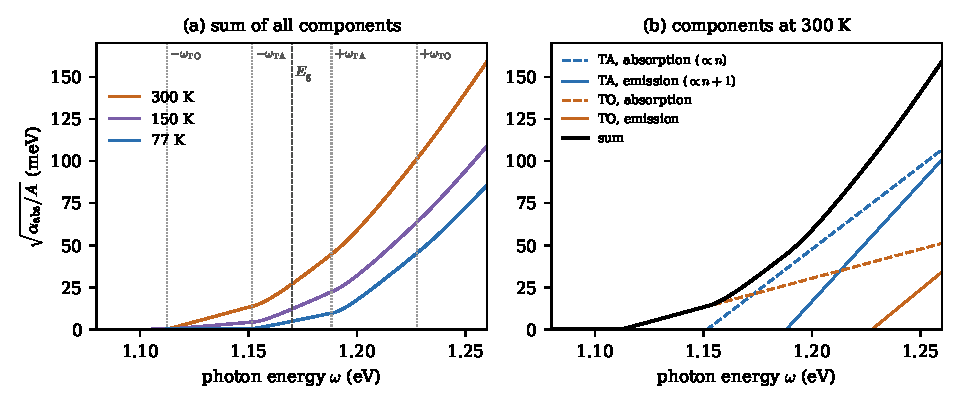
\includegraphics[width=\linewidth]{figures/ch06/fig6_8.pdf}
  \caption{The Hall--Bardeen--Blatt edge of silicon, \cref{eq:6.5-edge}, plotted as $\sqrt{\alpha_{\mathrm{abs}}/A}$ against the photon energy, with $\Eg = \SI{1.17}{eV}$ and the phonon energies $\omega_{\mathrm{TA}} = \SI{18.27}{meV}$ and $\omega_{\mathrm{TO}} = \SI{57.73}{meV}$ measured from the optical edge~\cite{macfarlane1958fine}. Dotted lines mark the free-pair thresholds $\Eg \mp \omega_{\mathrm{TO}}$ and $\Eg \mp \omega_{\mathrm{TA}}$; the dashed line marks $\Eg$, their common midpoint. (a) Sum of the four components at \SI{300}{K}, \SI{150}{K} and \SI{77}{K}. (b) The components at \SI{300}{K}: dashed, phonon absorption, proportional to $n_\nu$; solid, phonon emission, proportional to $n_\nu + 1$. Each component is a straight line; the sum (black) is not. The two branches are given equal coefficients $A_{\mathrm{TA}} = A_{\mathrm{TO}} = A$, so their relative heights are illustrative. The gap is held at its low-temperature value at every temperature, to isolate the phonon occupations (\cref{sec:6.3} treats its shift). The excitonic thresholds, \SI{14.7}{meV} lower, are omitted.}
  \label{fig:6-edge}
\end{figure}

\begin{workedexample}{The phonon thresholds of silicon}\label{we:6-siedge}
With $\Eg = \SI{1.17}{eV}$ and the phonon energies above, the four free-pair thresholds of \cref{eq:6.5-edge} are
\begin{equation*}
  \begin{gathered}
  \Eg - \omega_{\mathrm{TO}} = \SI{1.1123}{eV}, \qquad
  \Eg - \omega_{\mathrm{TA}} = \SI{1.1517}{eV}, \\
  \Eg + \omega_{\mathrm{TA}} = \SI{1.1883}{eV}, \qquad
  \Eg + \omega_{\mathrm{TO}} = \SI{1.2277}{eV} .
  \end{gathered}
\end{equation*}
The exciton binding $E_x^b = \SI{14.7}{meV}$ moves each of them down by that amount. The pairs of thresholds are symmetric about $\Eg$, separated by $2\omega_{\mathrm{TA}} = \SI{36.5}{meV}$ and $2\omega_{\mathrm{TO}} = \SI{115.5}{meV}$.

The slopes depend on the occupations alone, not on the gap. At \SI{300}{K}, $T = \SI{25.85}{meV}$, and
\begin{equation*}
  n_{\mathrm{TA}} = \frac{1}{\ee^{18.27/25.85} - 1} = 0.973, \qquad n_{\mathrm{TO}} = \frac{1}{\ee^{57.73/25.85} - 1} = 0.120 .
\end{equation*}
In units of $\sqrt{A_\nu}$, the transverse-acoustic components of $\sqrt{\alpha_{\mathrm{abs}}}$ rise with slopes $\sqrt{n_{\mathrm{TA}}} = 0.987$ (absorption) and $\sqrt{n_{\mathrm{TA}} + 1} = 1.405$ (emission), the transverse-optical ones with 0.346 and 1.058. The ratios of the slopes in each pair, 0.702 and 0.327, are $\ee^{-\omega_\nu/2T}$ for the two branches, independent of $A_\nu$. Read backwards, the transverse-acoustic ratio gives $-2T\ln 0.702 = \SI{18.27}{meV}$: the slope ratio of one branch returns its phonon energy if the temperature is known, or the temperature if the phonon energy is. At \SI{77}{K}, $T = \SI{6.635}{meV}$, the occupations fall to $n_{\mathrm{TA}} = 0.068$ and $n_{\mathrm{TO}} = 1.7\times10^{-4}$, and the slope ratios to 0.252 and 0.013. At \SI{20}{K} the transverse-acoustic absorption component has $n_{\mathrm{TA}} = 2.5\times10^{-5}$, and at the \SI{10}{mK} of a cryogenic detector $\omega_{\mathrm{TA}}/T = 2.1\times10^4$: the occupation is $\ee^{-21200}$, and only the emission thresholds exist. The lowest of them is the true optical edge of cold silicon, \SI{18}{meV} above the gap. With the measured low-temperature gap $\Eg(0) = \SI{1.1692}{eV}$ of \cref{sec:6.3} in place of the rounded value, this edge lies at $\Eg(0) + \omega_{\mathrm{TA}} = \SI{1.1875}{eV}$ for a free pair, and the excitonic edge at \SI{1.1728}{eV}, since $\omega_{\mathrm{TA}}$ and $E_x^b$ nearly cancel.
\end{workedexample}

\subsection{Phonon-assisted dark-matter scattering}

The derivation of \cref{eq:6.5-M} used only two properties of the photon: it couples to the electrons through a one-body operator, and it carries negligible momentum. A dark-matter particle that interacts with the electron density keeps the first property and loses the second. Its vertex is the dark-matter potential $\tilde V(\vect{q})$ times the matrix element of $n_e(\vect{q}) = \int\dd^3r\,\ee^{\ii\vect{q}\cdot\vect{r}}\,\op{\nd}_e(\vect{r})$, the Fourier component of the density operator. Between Bloch states this matrix element is the density vertex $\rho_{mn}(\vect{k},\vect{q})$ of \cref{eq:3.2-rho}. The optical vertex $\hat{\vect{e}}_\gamma\cdot\vect{v}_{pv}(\vect{k})$ is replaced by $\rho_{pv}(\vect{k},\vect{q})$, which is no longer vertical: it takes the electron from $\vect{k}$ to $\vect{k} + \vect{q}$. The phonon then supplies the rest of the crystal momentum, $\vect{Q} = \vect{k}_{\mathrm{c}} - \vect{q}$ up to a reciprocal-lattice vector for a transition from the valence maximum to a valley. The amplitude has the same orderings and the same hole paths, but its vertices and energies are evaluated at three crystal momenta, $\vect{k}$, $\vect{k} + \vect{q}$ and $\vect{k} + \vect{q} + \vect{Q}$, instead of two.

The energy denominators take the energy deposited $\omega$ in place of the photon energy, and they resonate wherever $\omega$ matches a real pair at momentum transfer $\vect{q}$, with the same risk of double counting as at $E_{\mathrm{dir}}$. Since $\rho_{mn}$ reduces to the optical vertex as $q \to 0$ (\cref{eq:3.2-optical}), the measured silicon edge is the zero-momentum limit of the dark-matter amplitude and a test of any calculation of it.

Absorbed bosons and scattering particles meet this amplitude in different limits. An absorbed boson, a kinetically mixed dark photon for instance, deposits its whole mass with a momentum $m_\phi v \approx 10^{-3}m_\phi$, a smaller momentum for its energy than a photon carries. Its absorption between $\Eg$ and $E_{\mathrm{dir}}$ is \cref{eq:6.5-eps2PA} with the photon's coupling replaced by its own and screened by the medium (\cref{sec:8.4-mixing}). A scattering particle transfers $\vect{q}$ and $\omega$ together, with $\omega \le qv_{\mathrm{max}} - q^2/2\mchi$ (\cref{eq:1.3-region}). Far above its threshold mass it reaches $\vect{k}_{\mathrm{c}}$ at first order, but just above the threshold mass the energy needed to cross the gap is available at momentum transfers well below $k_{\mathrm{c}}$, where the zero-phonon transition is forbidden (\cref{sec:3.3}). At the threshold mass, $\omega = \Eg$ is reached just at $q = 2\Eg/v_{\mathrm{max}} = \SI{0.88}{keV}$, and for heavier dark matter the smallest such $q$ falls toward $\Eg/v_{\mathrm{max}} = \SI{0.44}{keV}$; both lie well below $k_{\mathrm{c}} = 0.85\,(2\pi/a) = \SI{1.9}{keV}$. At these momentum transfers, as for light below $E_{\mathrm{dir}}$, the phonon-assisted amplitude is the leading process, and it opens a window of masses in which silicon sees dark matter only through the phonon-assisted process. In a cold detector, however, only the emission branch contributes: the phonon takes part of the energy deposited, and the pair receives $\omega - \omega_{\vect{Q}\nu}$.

\section*{Summary}

The Born--Oppenheimer approximation keeps only the diagonal of the coupling between electrons and nuclei, and the off-diagonal coupling follows from the derivative-coupling vector $\vect{d}_{ji} = \langle\Psi_j|\nabla\Psi_i\rangle$ (\cref{sec:6.1}). To first order in the displacements the same physics is the electron--phonon Hamiltonian $H_{\mathrm{ep}}$, in which a phonon of wavevector $\vect{Q}$ moves an electron from $\vect{k}$ to $\vect{k} + \vect{Q}$ with the vertex $g_{mn\nu}(\vect{k},\vect{Q})$. Whether the electrons follow a moving nucleus depends on how fast the nucleus is accelerated. If the acceleration is slow compared with $1/\Delta E$, the electrons stay in their ground state. If it is sudden, they keep their state while the nucleus acquires a velocity $v_N$, and the complement of the overlap of the boosted ground state with the original one is the Migdal effect.

The vertex that density-functional perturbation theory computes is screened (\cref{sec:6.2}). Acoustic phonons couple through deformation potentials, with $g \propto Q^{1/2}$, optical phonons in nonpolar crystals through optical deformation potentials, and longitudinal optical phonons in polar crystals through the Fr\"ohlich vertex $g^{\mathrm{L}} = \ii C_{\mathrm{F}}\rho_{mn}/Q$, which in GaAs gives a polaron constant $\alpha_{\mathrm{F}} = 0.072$.

Second order in the displacements yields the electron self-energy, the Fan--Migdal and Allen--Heine terms, which in the adiabatic limit combine into the average of the band energy over the zero-point and thermal smearing of the lattice (\cref{sec:6.3}). For the indirect gap of silicon the computed zero-point renormalization is \SI{-56.2}{meV}; the measured electron--phonon part, $-71$ to \SI{-73}{meV}, is about \SI{20}{\percent} larger. A detector at \SI{10}{mK} sees the low-temperature gap, which already contains the full renormalization.

Photons between the indirect gap of silicon and its direct gap of \SI{3.4}{eV} are absorbed only with a phonon (\cref{sec:6.5}). Summed over electron and phonon wavevectors in the whole zone, the squared second-order amplitude $|M^\pm|^2$ gives the phonon-assisted dielectric function $\varepsilon_2^{\mathrm{PA}}$. Near the edge it reduces to the Hall--Bardeen--Blatt law, each phonon branch adding components growing as $(\omega - \Eg \pm \omega_\nu)^2$, and in a cold detector only emission survives. Replacing the optical vertex by the density vertex turns phonon-assisted absorption of light into the phonon-assisted response to dark matter, which governs the absorption of light bosons (\cref{sec:13.8}) and the threshold window of electron recoils in silicon.

A phonon decays into electron--hole pairs only where real pairs exist at its energy (\cref{sec:6.4}). Its self-energy is the electron bubble, whose static part is already contained in the frequencies of density-functional perturbation theory. In a metal the imaginary part leads to Allen's formula, the Eliashberg function $\alpha^2F(\omega)$ and the coupling constant $\lambda_{\mathrm{ep}}$. For aluminum a free-electron model with one core radius yields $\lambda_{\mathrm{ep}} = 0.436$, against 0.42 to 0.43 from tunneling and the specific heat, and $\lambda_{\mathrm{ep}}$ sets the strength of the pairing in the superconducting sensors of \cref{chap:7}.

\printbibliography[heading=subbibliography]
